% ============================================================
%  CS 464 Final Project Report — Group 24
%  Interpretable Stroke Risk Prediction
% ============================================================
\documentclass[11pt,a4paper]{article}

% ---------- Encoding & fonts ----------
\usepackage[T1]{fontenc}
\usepackage[utf8]{inputenc}
\usepackage{lmodern}
\usepackage{microtype}

% ---------- Page geometry ----------
\usepackage[
  top=2.5cm, bottom=2.5cm,
  left=2.8cm, right=2.8cm
]{geometry}

% ---------- Math ----------
\usepackage{amsmath,amssymb}

% ---------- Graphics & colors ----------
\usepackage{graphicx}
\usepackage[dvipsnames,svgnames,table]{xcolor}
\graphicspath{{./}{outputs/figures/}}

% ---------- Tables ----------
\usepackage{booktabs}
\usepackage{multirow}
\usepackage{array}
\usepackage{tabularx}
\usepackage{makecell}

% ---------- Captions & figures ----------
\usepackage{caption}
\usepackage{subcaption}
\usepackage{float}
\captionsetup{font=small, labelfont=bf}

% ---------- Headers & footers ----------
\usepackage{fancyhdr}
\fancypagestyle{main}{%
  \fancyhf{}
  \fancyhead[L]{\small\itshape Interpretable Stroke Risk Prediction on Tabular Clinical Data}
  \fancyhead[R]{\small\thepage}
  \renewcommand{\headrulewidth}{0.4pt}
  \renewcommand{\footrulewidth}{0pt}
}
\pagestyle{main}

% ---------- Section titles ----------
\usepackage{titlesec}
\definecolor{headingblue}{HTML}{1A4E8A}
\titleformat{\section}{\large\bfseries\color{headingblue}}{\thesection}{1em}{}
\titleformat{\subsection}{\normalsize\bfseries\color{headingblue!80}}{\thesubsection}{1em}{}
\titleformat{\subsubsection}{\normalsize\itshape}{\thesubsubsection}{1em}{}

% ---------- Lists ----------
\usepackage{enumitem}
\setlist[itemize]{noitemsep, topsep=3pt}
\setlist[enumerate]{noitemsep, topsep=3pt}

% ---------- References ----------
\usepackage[numbers,sort&compress]{natbib}
\bibliographystyle{abbrvnat}

% ---------- Hyperlinks (load last) ----------
\usepackage[
  colorlinks=true,
  linkcolor=headingblue,
  citecolor=teal,
  urlcolor=teal
]{hyperref}

% ---------- Convenience macros ----------
\newcommand{\auc}{\text{AUC-PR}}
\newcommand{\pct}[1]{#1\%}

% ============================================================
\begin{document}

% ==================== TITLE PAGE ====================
\begin{titlepage}
  \thispagestyle{empty}
  \centering
  \vspace*{0.8cm}
  
\includegraphics[width=0.42\linewidth]{bilkent_logo.png}\par
  \vspace{0.9cm}
  {\large\textbf{CS 464 — Introduction to Machine Learning}\par}
  {\large Spring 2026 \textbar{} Section 3 — Group 24\par}
  \vspace{1.2cm}
  \rule{\linewidth}{1.5pt}\vspace{0.4cm}
  {\LARGE\bfseries\color{headingblue}
    Interpretable Stroke Risk Prediction\\
    on Tabular Clinical Data\par}
  \vspace{0.4cm}\rule{\linewidth}{1.5pt}
  \vspace{1.5cm}

  \begin{tabular}{lll}
    \toprule
    \textbf{Name} & \textbf{Student ID} & \textbf{E-mail} \\
    \midrule
    Nevzat Han Alt\i{}n    & 22202085 & han.altin@ug.bilkent.edu.tr \\
    Ahmet B\"uy\"ukberber  & 22202896 & ahmet.buyukberber@ug.bilkent.edu.tr \\
    Veli Karakaya          & 22202039 & veli.karakaya@ug.bilkent.edu.tr \\
    Ece \c{S}e\c{s}en     & 22201637 & ece.sesen@ug.bilkent.edu.tr \\
    Umut \c{C}a\u{g}\i{}n \"Ozcan & 22203549 & cagin.ozcan@ug.bilkent.edu.tr \\
    \bottomrule
  \end{tabular}
  \vfill
\end{titlepage}

\clearpage
\thispagestyle{empty}
\tableofcontents
\clearpage

% ============================================================
\section{Introduction}
\label{sec:intro}
% ============================================================

Stroke is the second leading cause of death globally and a major cause of long-term disability~\cite{feigin2021global}.
Early identification of at-risk individuals enables preventive intervention, yet clinical risk assessment tools are often rule-based and limited in personalisation.
Machine learning offers a data-driven alternative; however, two fundamental challenges arise when training models on clinical stroke datasets:

\begin{enumerate}
  \item \textbf{Severe class imbalance.}
        In the dataset used here, only $4.87\%$ of patients experienced a stroke.
        A classifier that always predicts ``no stroke'' achieves $95.1\%$ accuracy while detecting \emph{zero} stroke cases—the \emph{accuracy paradox}.

  \item \textbf{Clinical calibration requirements.}
        A deployed model must produce reliable probability estimates, not just binary predictions, so that clinicians can triage patients according to risk level.
\end{enumerate}

\textbf{Objectives.}
This project aims to:
\begin{itemize}
  \item Demonstrate the accuracy paradox on a real clinical dataset.
  \item Evaluate four complementary imbalance-handling strategies and compare them across multiple model families.
  \item Identify the best pipeline configuration through a systematic hyperparameter search.
  \item Analyse prediction quality via calibration curves and feature importance (SHAP / LIME).
\end{itemize}

Throughout this work we treat \textbf{AUC-PR} (area under the precision-recall curve) as the primary evaluation metric, because it is more sensitive to minority-class performance than AUC-ROC under severe imbalance~\cite{davis2006relationship}.

% ============================================================
\section{Dataset}
\label{sec:dataset}
% ============================================================

\subsection{Dataset Analysis}

\subsubsection{Source and Overview}

We use the publicly available \textit{Healthcare Stroke Prediction Dataset}~\cite{fedesoriano2021stroke} from Kaggle.
Table~\ref{tab:dataset_summary} summarises its key statistics.

\begin{table}[H]
  \centering
  \caption{Dataset overview.}
  \label{tab:dataset_summary}
  \begin{tabular}{lp{9cm}}
    \toprule
    \textbf{Property} & \textbf{Value} \\
    \midrule
    Total samples & 5{,}110 \\
    Stroke cases (positive class) & 249 ($4.87\%$) \\
    Non-stroke cases (negative class) & 4{,}861 ($95.13\%$) \\
    Features & 11 clinical + 1 target \\
    Numeric features & 3 (\texttt{age}, \texttt{avg\_glucose\_level}, \texttt{bmi}) \\
    Categorical features & 5 (\texttt{gender}, \texttt{ever\_married}, \texttt{work\_type}, \texttt{Residence\_type}, \texttt{smoking\_status}) \\
    Binary features & 2 (\texttt{hypertension}, \texttt{heart\_disease}) \\
    Dropped feature & \texttt{id} (identifier only) \\
    \bottomrule
  \end{tabular}
\end{table}

\subsubsection{Class Imbalance}

Figure~\ref{fig:class_dist} illustrates the severe imbalance: the minority class (stroke) represents less than one in twenty patients.
This ratio is the central challenge of the project and motivates all modelling decisions that follow.

\begin{figure}[H]
  \centering
  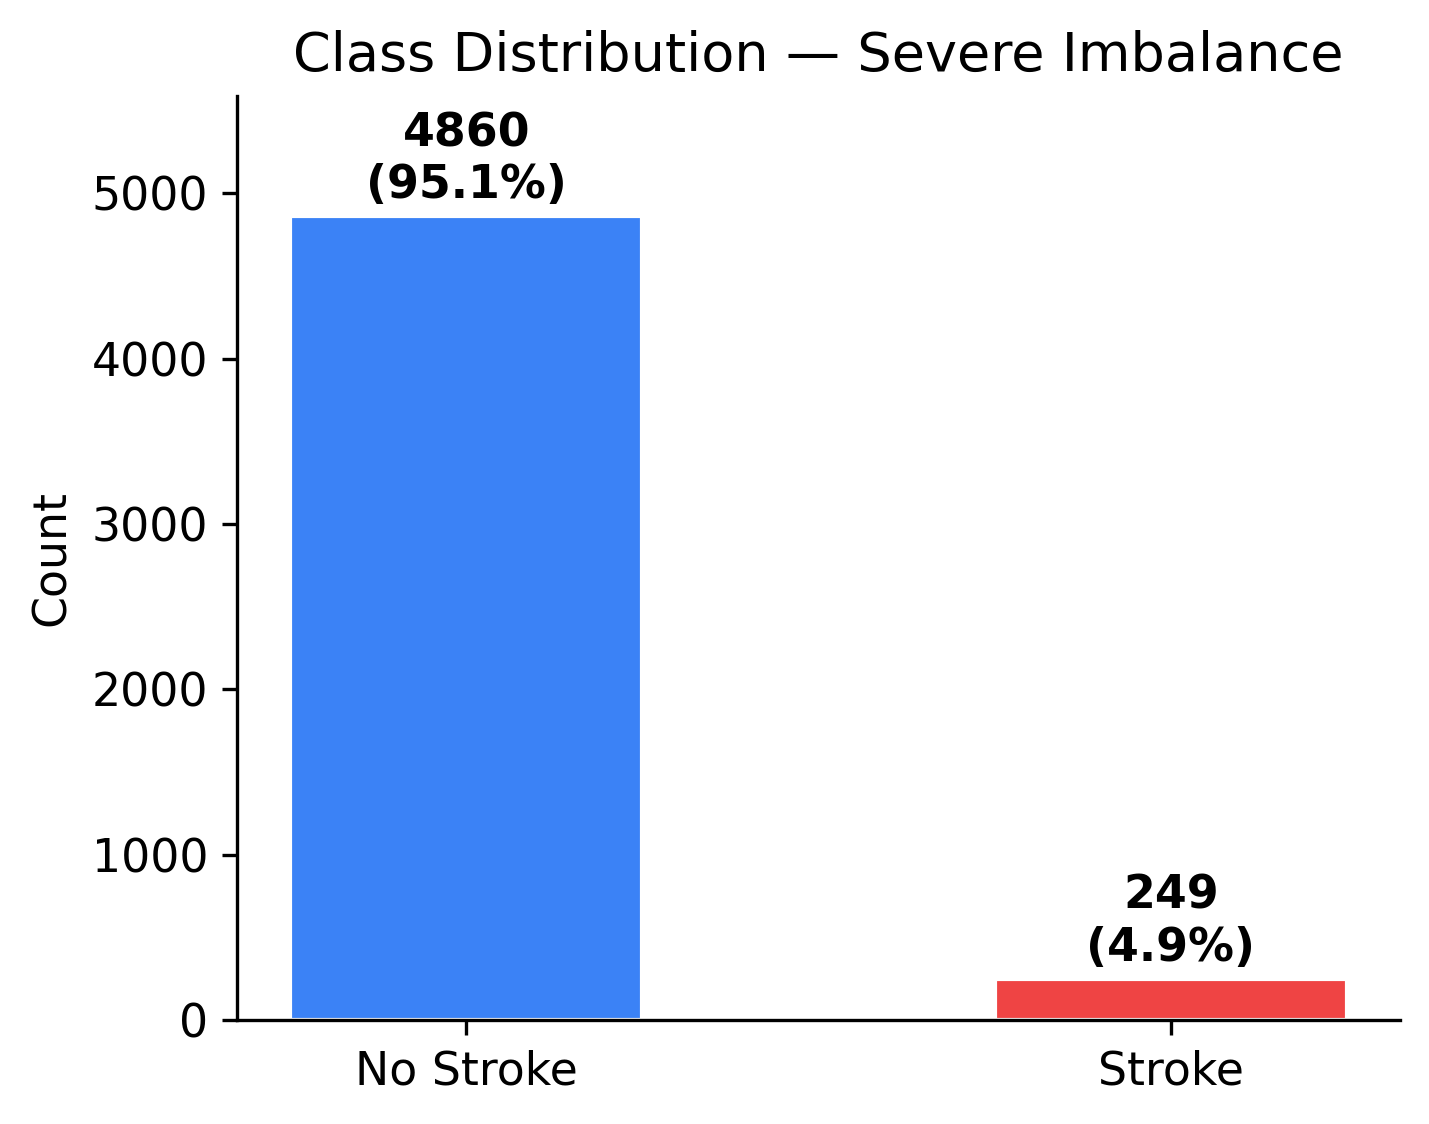
\includegraphics[width=0.52\linewidth]{01_class_distribution.png}
  \caption{Class distribution. The stroke class ($4.87\%$) is severely under-represented.}
  \label{fig:class_dist}
\end{figure}

\subsubsection{Continuous Feature Distributions}

Figure~\ref{fig:kde} shows kernel-density estimates of the three continuous features, stratified by stroke status.

\begin{figure}[H]
  \centering
  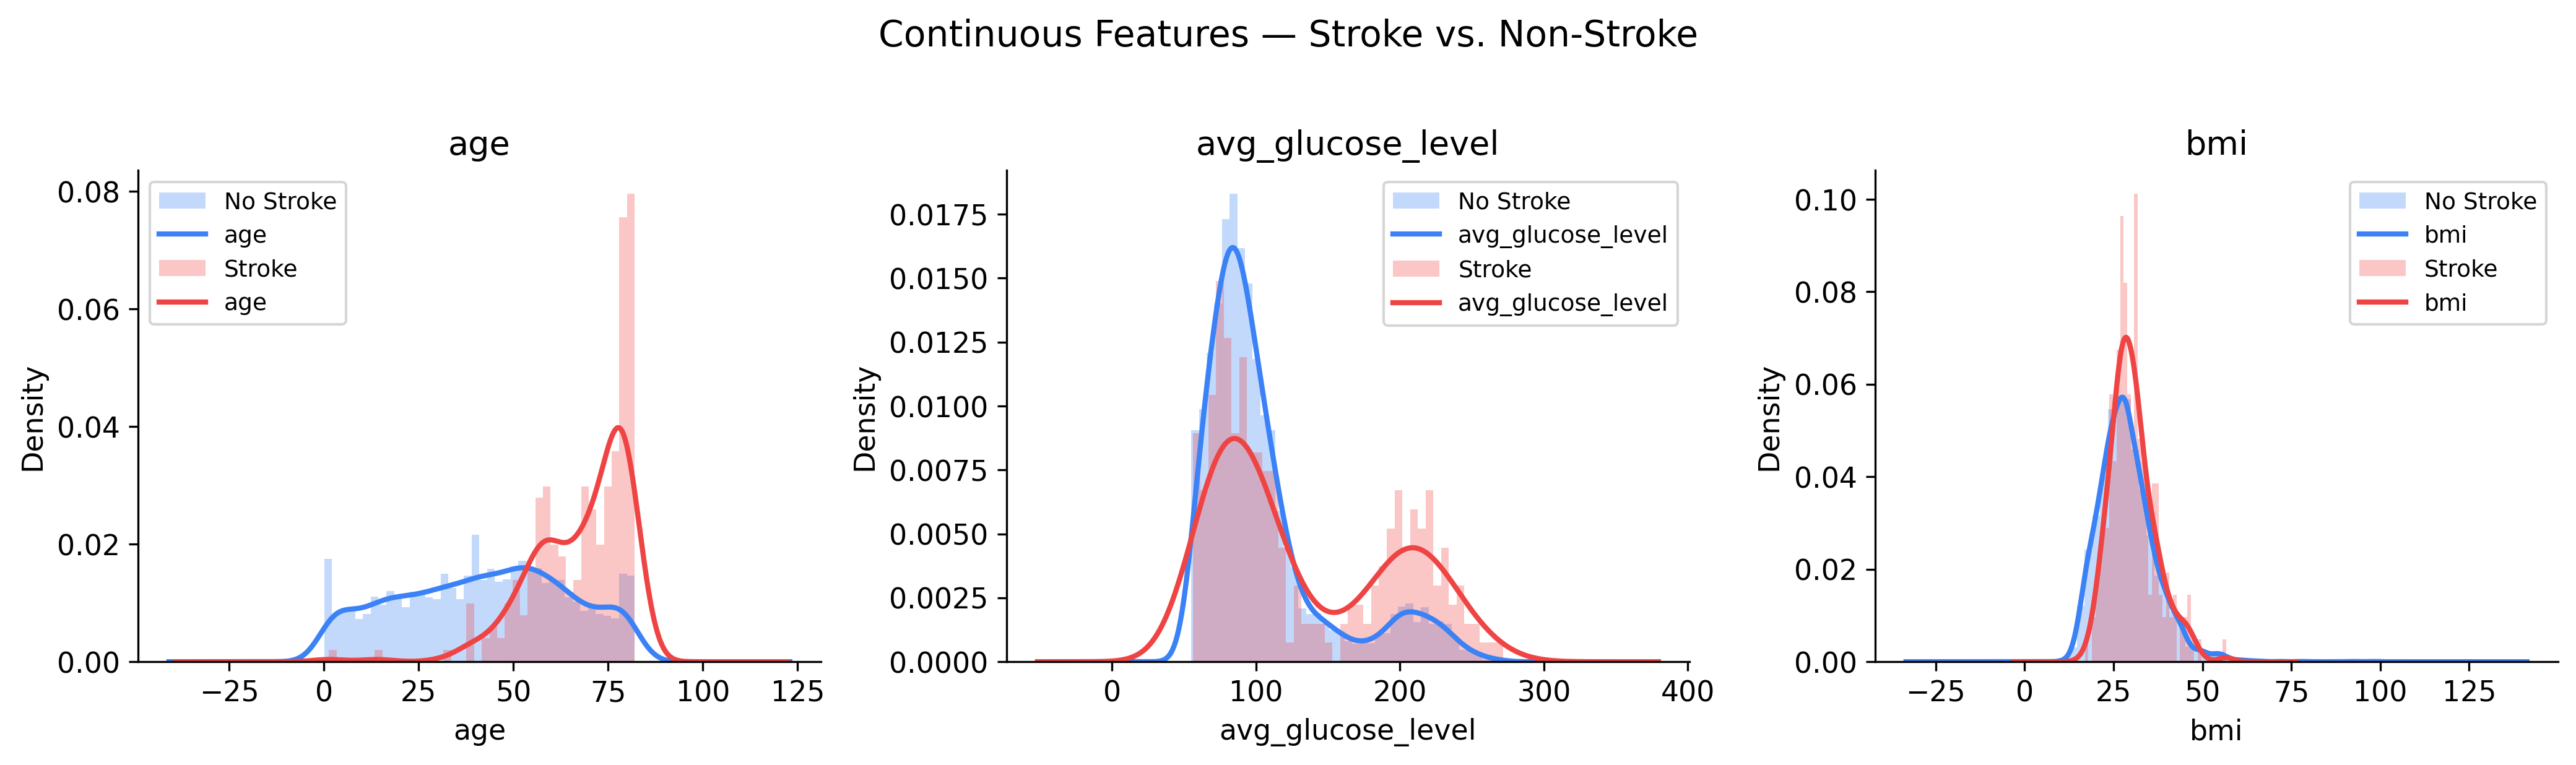
\includegraphics[width=0.88\linewidth]{02_continuous_kde.png}
  \caption{KDE plots of continuous features by stroke status. Stroke patients are considerably older and show higher glucose levels on average.}
  \label{fig:kde}
\end{figure}

The means and standard deviations by class are given in Table~\ref{tab:continuous_stats}.

\begin{table}[H]
  \centering
  \caption{Continuous feature statistics stratified by stroke outcome.}
  \label{tab:continuous_stats}
  \begin{tabular}{lccc}
    \toprule
    \textbf{Feature} & \textbf{No Stroke} & \textbf{Stroke} & \textbf{Diff.} \\
    & \textbf{(mean $\pm$ std)} & \textbf{(mean $\pm$ std)} & \\
    \midrule
    Age (years)                & $41.97 \pm 22.29$ & $67.73 \pm 12.73$ & $+25.76$ \\
    Avg.\ glucose (mg/dL)      & $104.79 \pm 43.85$ & $132.54 \pm 61.92$ & $+27.75$ \\
    BMI (kg/m\textsuperscript{2}) & $28.82 \pm 7.91$ & $30.47 \pm 6.33$ & $+1.65$ \\
    \bottomrule
  \end{tabular}
\end{table}

\subsubsection{Categorical Feature Analysis}

Figure~\ref{fig:cat_rates} shows stroke rates across all categorical variables.

\begin{figure}[H]
  \centering
  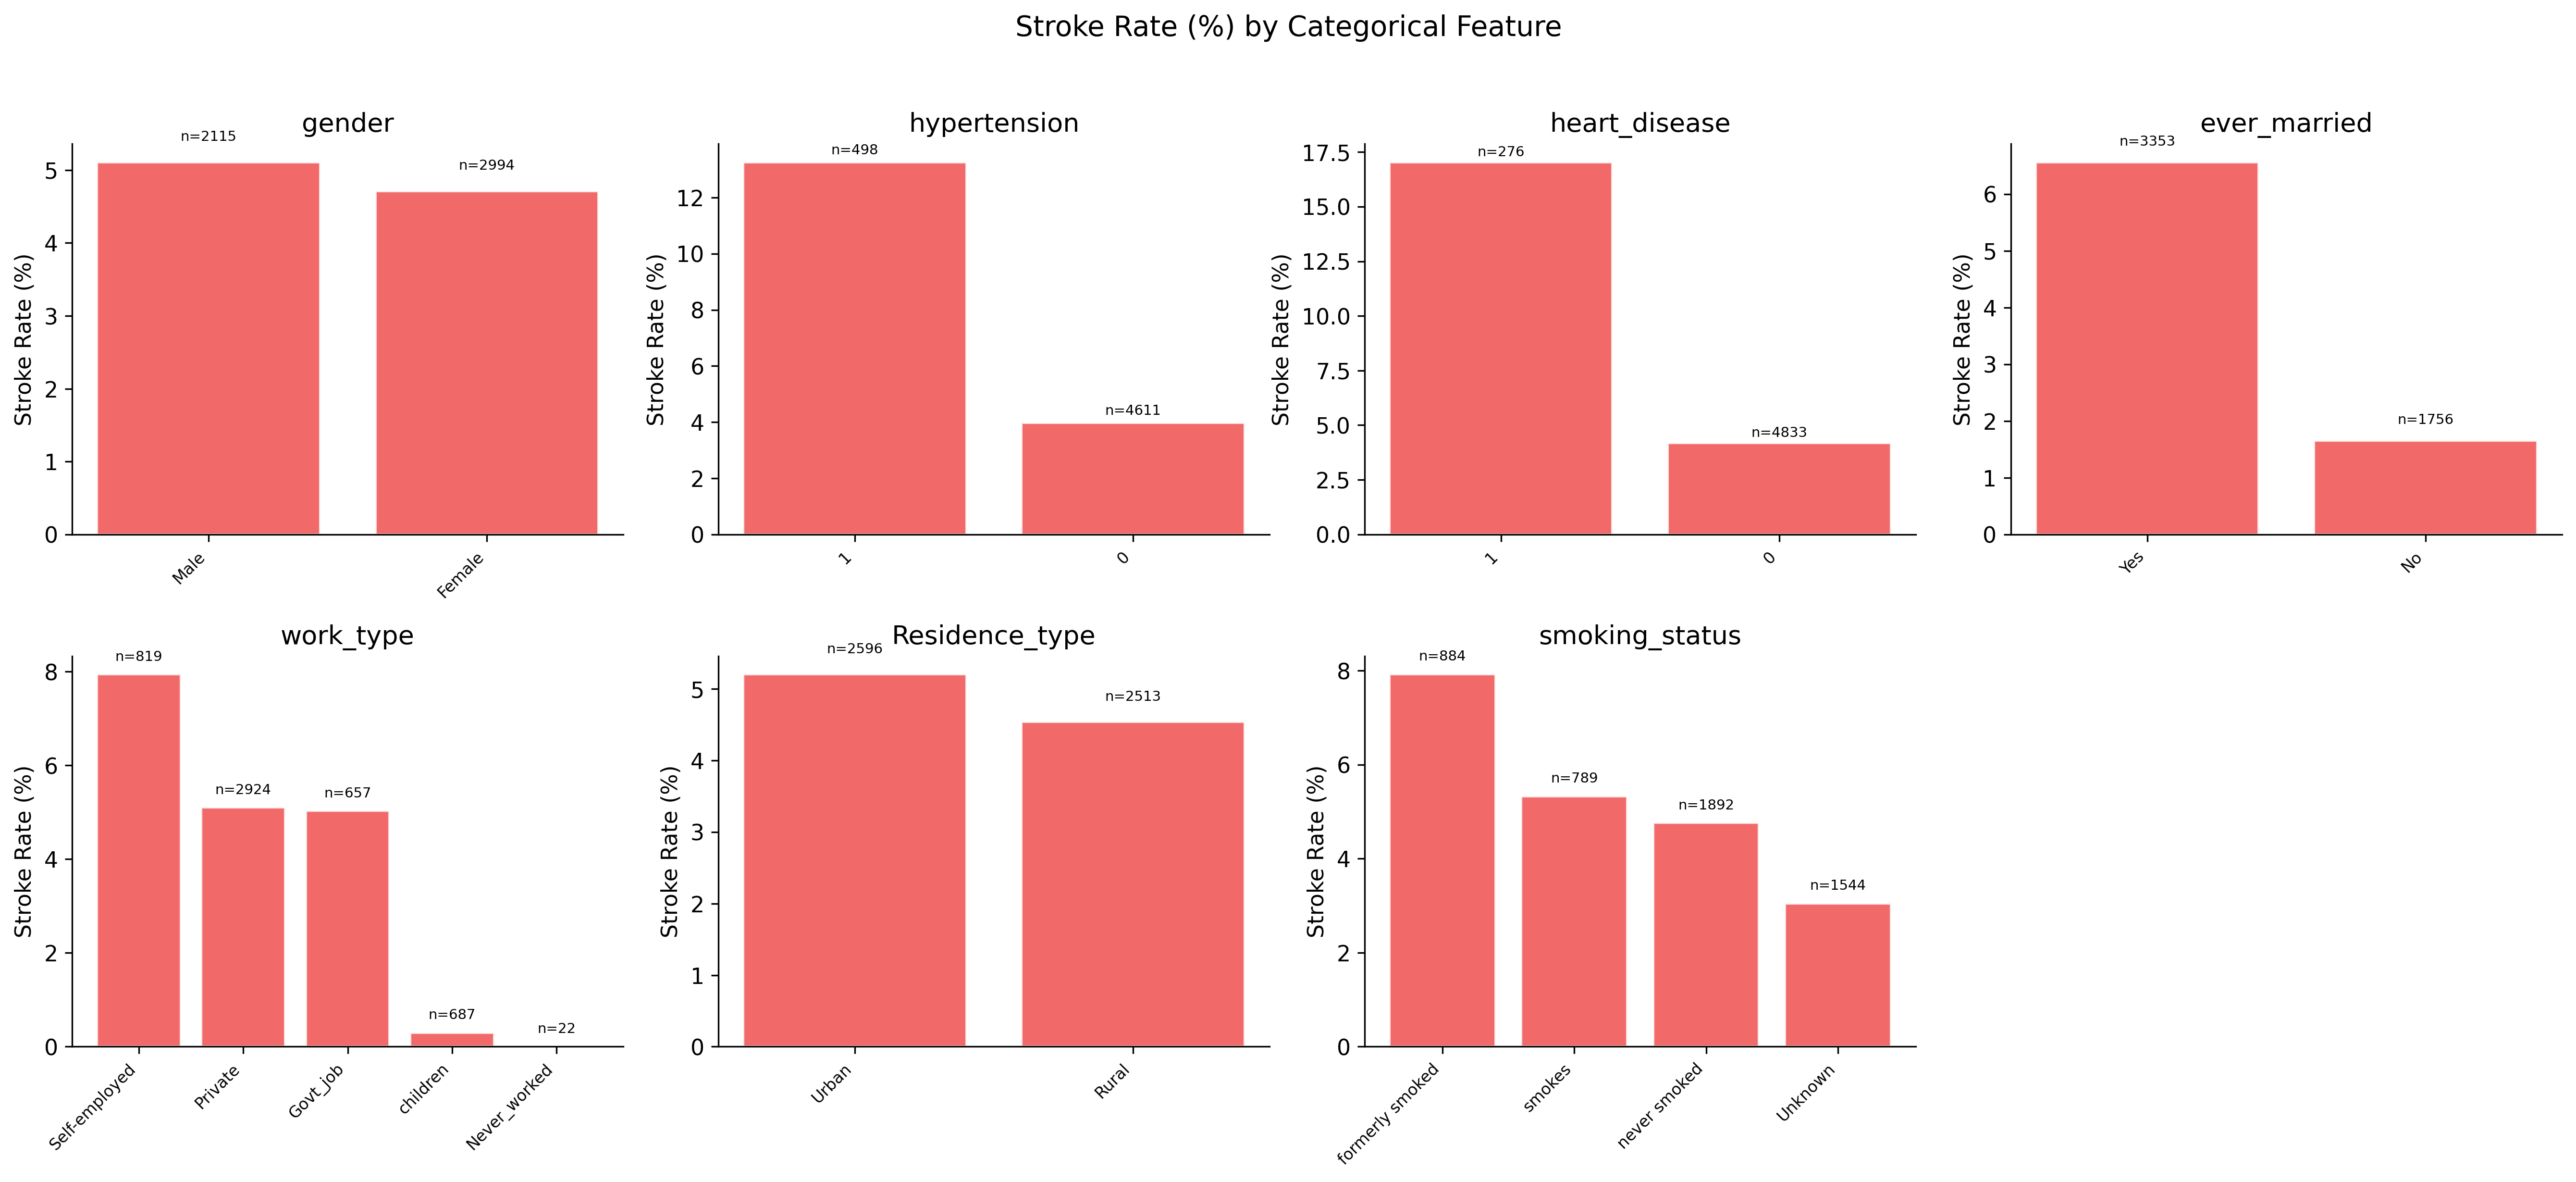
\includegraphics[width=0.88\linewidth]{03_categorical_stroke_rates.png}
  \caption{Stroke rate by categorical feature level. Hypertension, heart disease, and marriage status show the clearest associations.}
  \label{fig:cat_rates}
\end{figure}

\subsubsection{Statistical Significance Tests}

Table~\ref{tab:stat_tests} summarises formal statistical tests comparing stroke and non-stroke groups.

\begin{table}[H]
  \centering
  \caption{Statistical tests for association between each feature and stroke outcome.}
  \label{tab:stat_tests}
  \renewcommand{\arraystretch}{1.15}
  \begin{tabular}{lp{3cm}ccc}
    \toprule
    \textbf{Feature} & \textbf{Test} & \textbf{$p$-value} & \textbf{Effect size} & \textbf{Sig.?} \\
    \midrule
    Age               & Mann-Whitney $U$ & $3.85\times10^{-71}$ & $r_{rb}=0.669$ & Yes \\
    Avg.\ glucose     & Mann-Whitney $U$ & $3.58\times10^{-9}$ & $r_{rb}=0.221$ & Yes \\
    BMI               & Mann-Whitney $U$ & $1.04\times10^{-4}$ & $r_{rb}=0.158$ & Yes \\
    Hypertension      & $\chi^{2}$ (81.57) & $1.69\times10^{-19}$ & OR$=3.70$ [2.74–4.98] & Yes \\
    Heart disease     & $\chi^{2}$ (90.23) & $2.12\times10^{-21}$ & OR$=4.71$ [3.34–6.64] & Yes \\
    Ever married      & $\chi^{2}$ (58.87) & $1.69\times10^{-14}$ & OR$=4.18$ [2.83–6.19] & Yes \\
    Work type         & $\chi^{2}$ (49.16) & $5.41\times10^{-10}$ & Cramér's $V$ & Yes \\
    Smoking status    & $\chi^{2}$ (29.23) & $2.01\times10^{-6}$ & $V=0.076$ & Yes \\
    Gender            & $\chi^{2}$        & $p=0.56$ & — & No \\
    Residence type    & $\chi^{2}$        & $p=0.30$ & — & No \\
    \bottomrule
  \end{tabular}
\end{table}

Age is by far the strongest predictor ($r_{rb}=0.669$), followed by the presence of heart disease (OR$=4.71$) and hypertension (OR$=3.70$).
Gender and residence type are not statistically significant.

\subsubsection{Feature Correlation and Missing Data}

\begin{figure}[H]
  \centering
  \begin{subfigure}[b]{0.48\linewidth}
    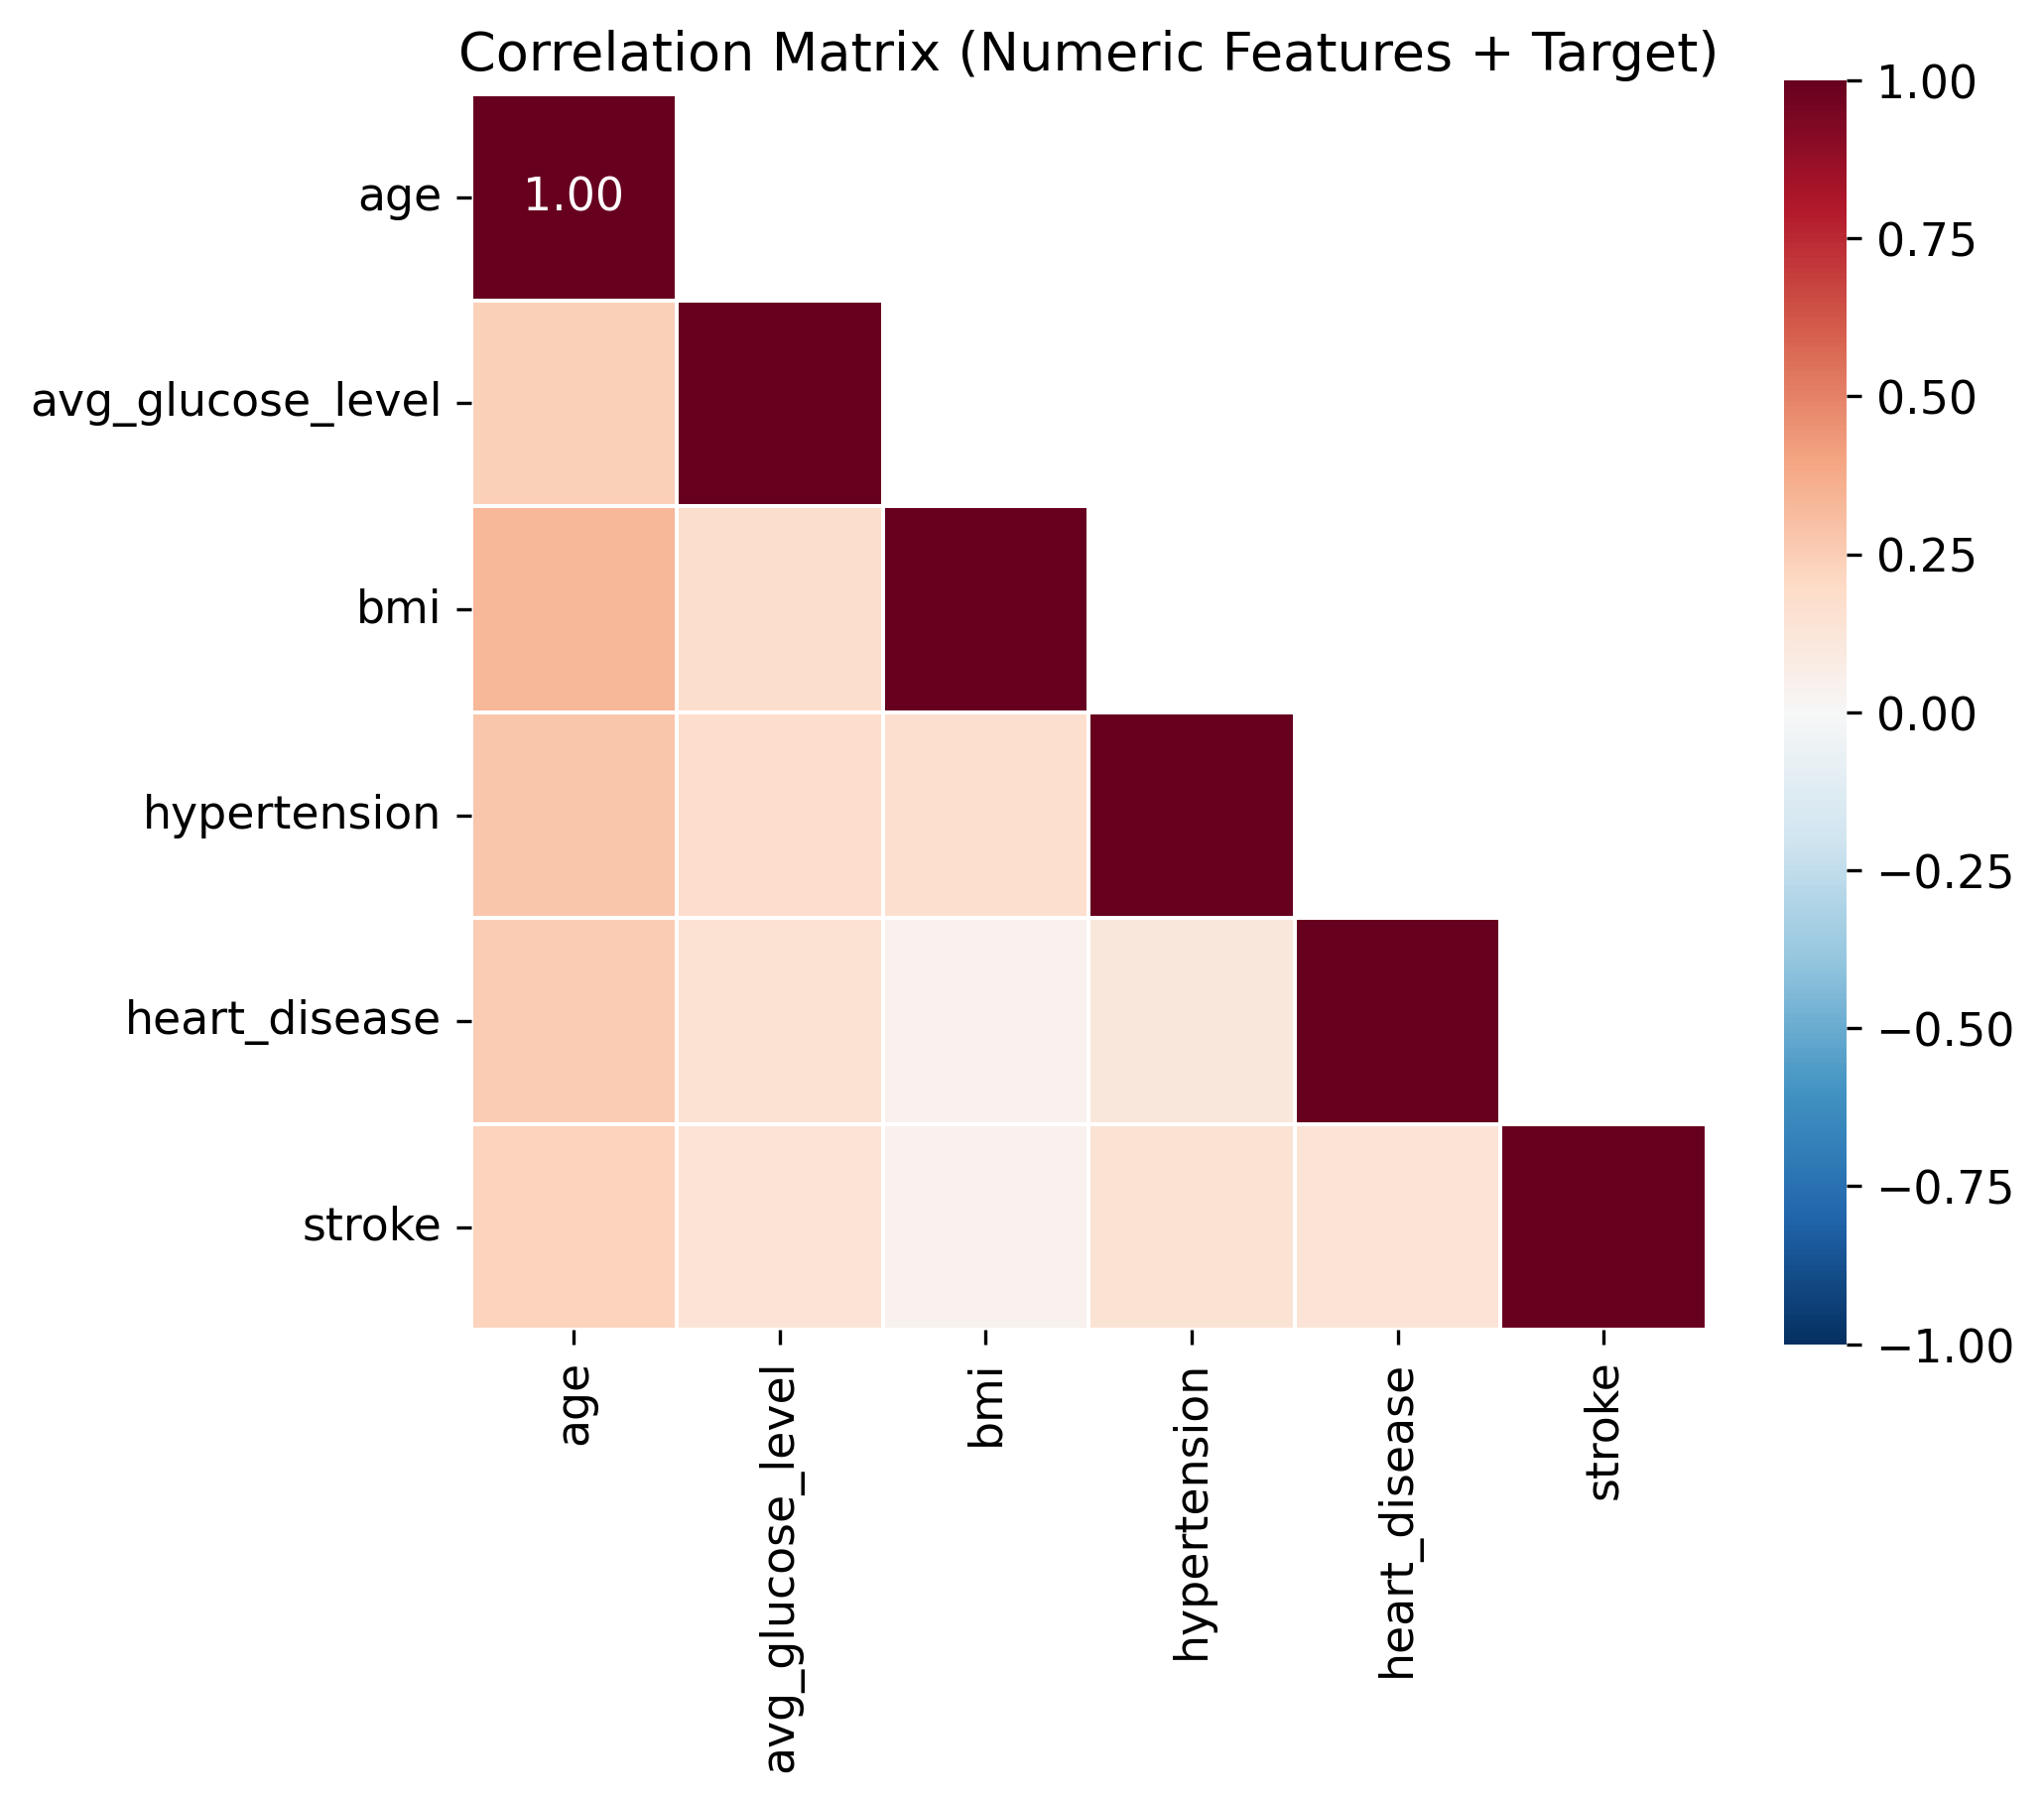
\includegraphics[width=\linewidth]{05_correlation_heatmap.png}
    \caption{Numeric feature correlation heatmap.}
    \label{fig:corr}
  \end{subfigure}
  \hfill
  \begin{subfigure}[b]{0.48\linewidth}
    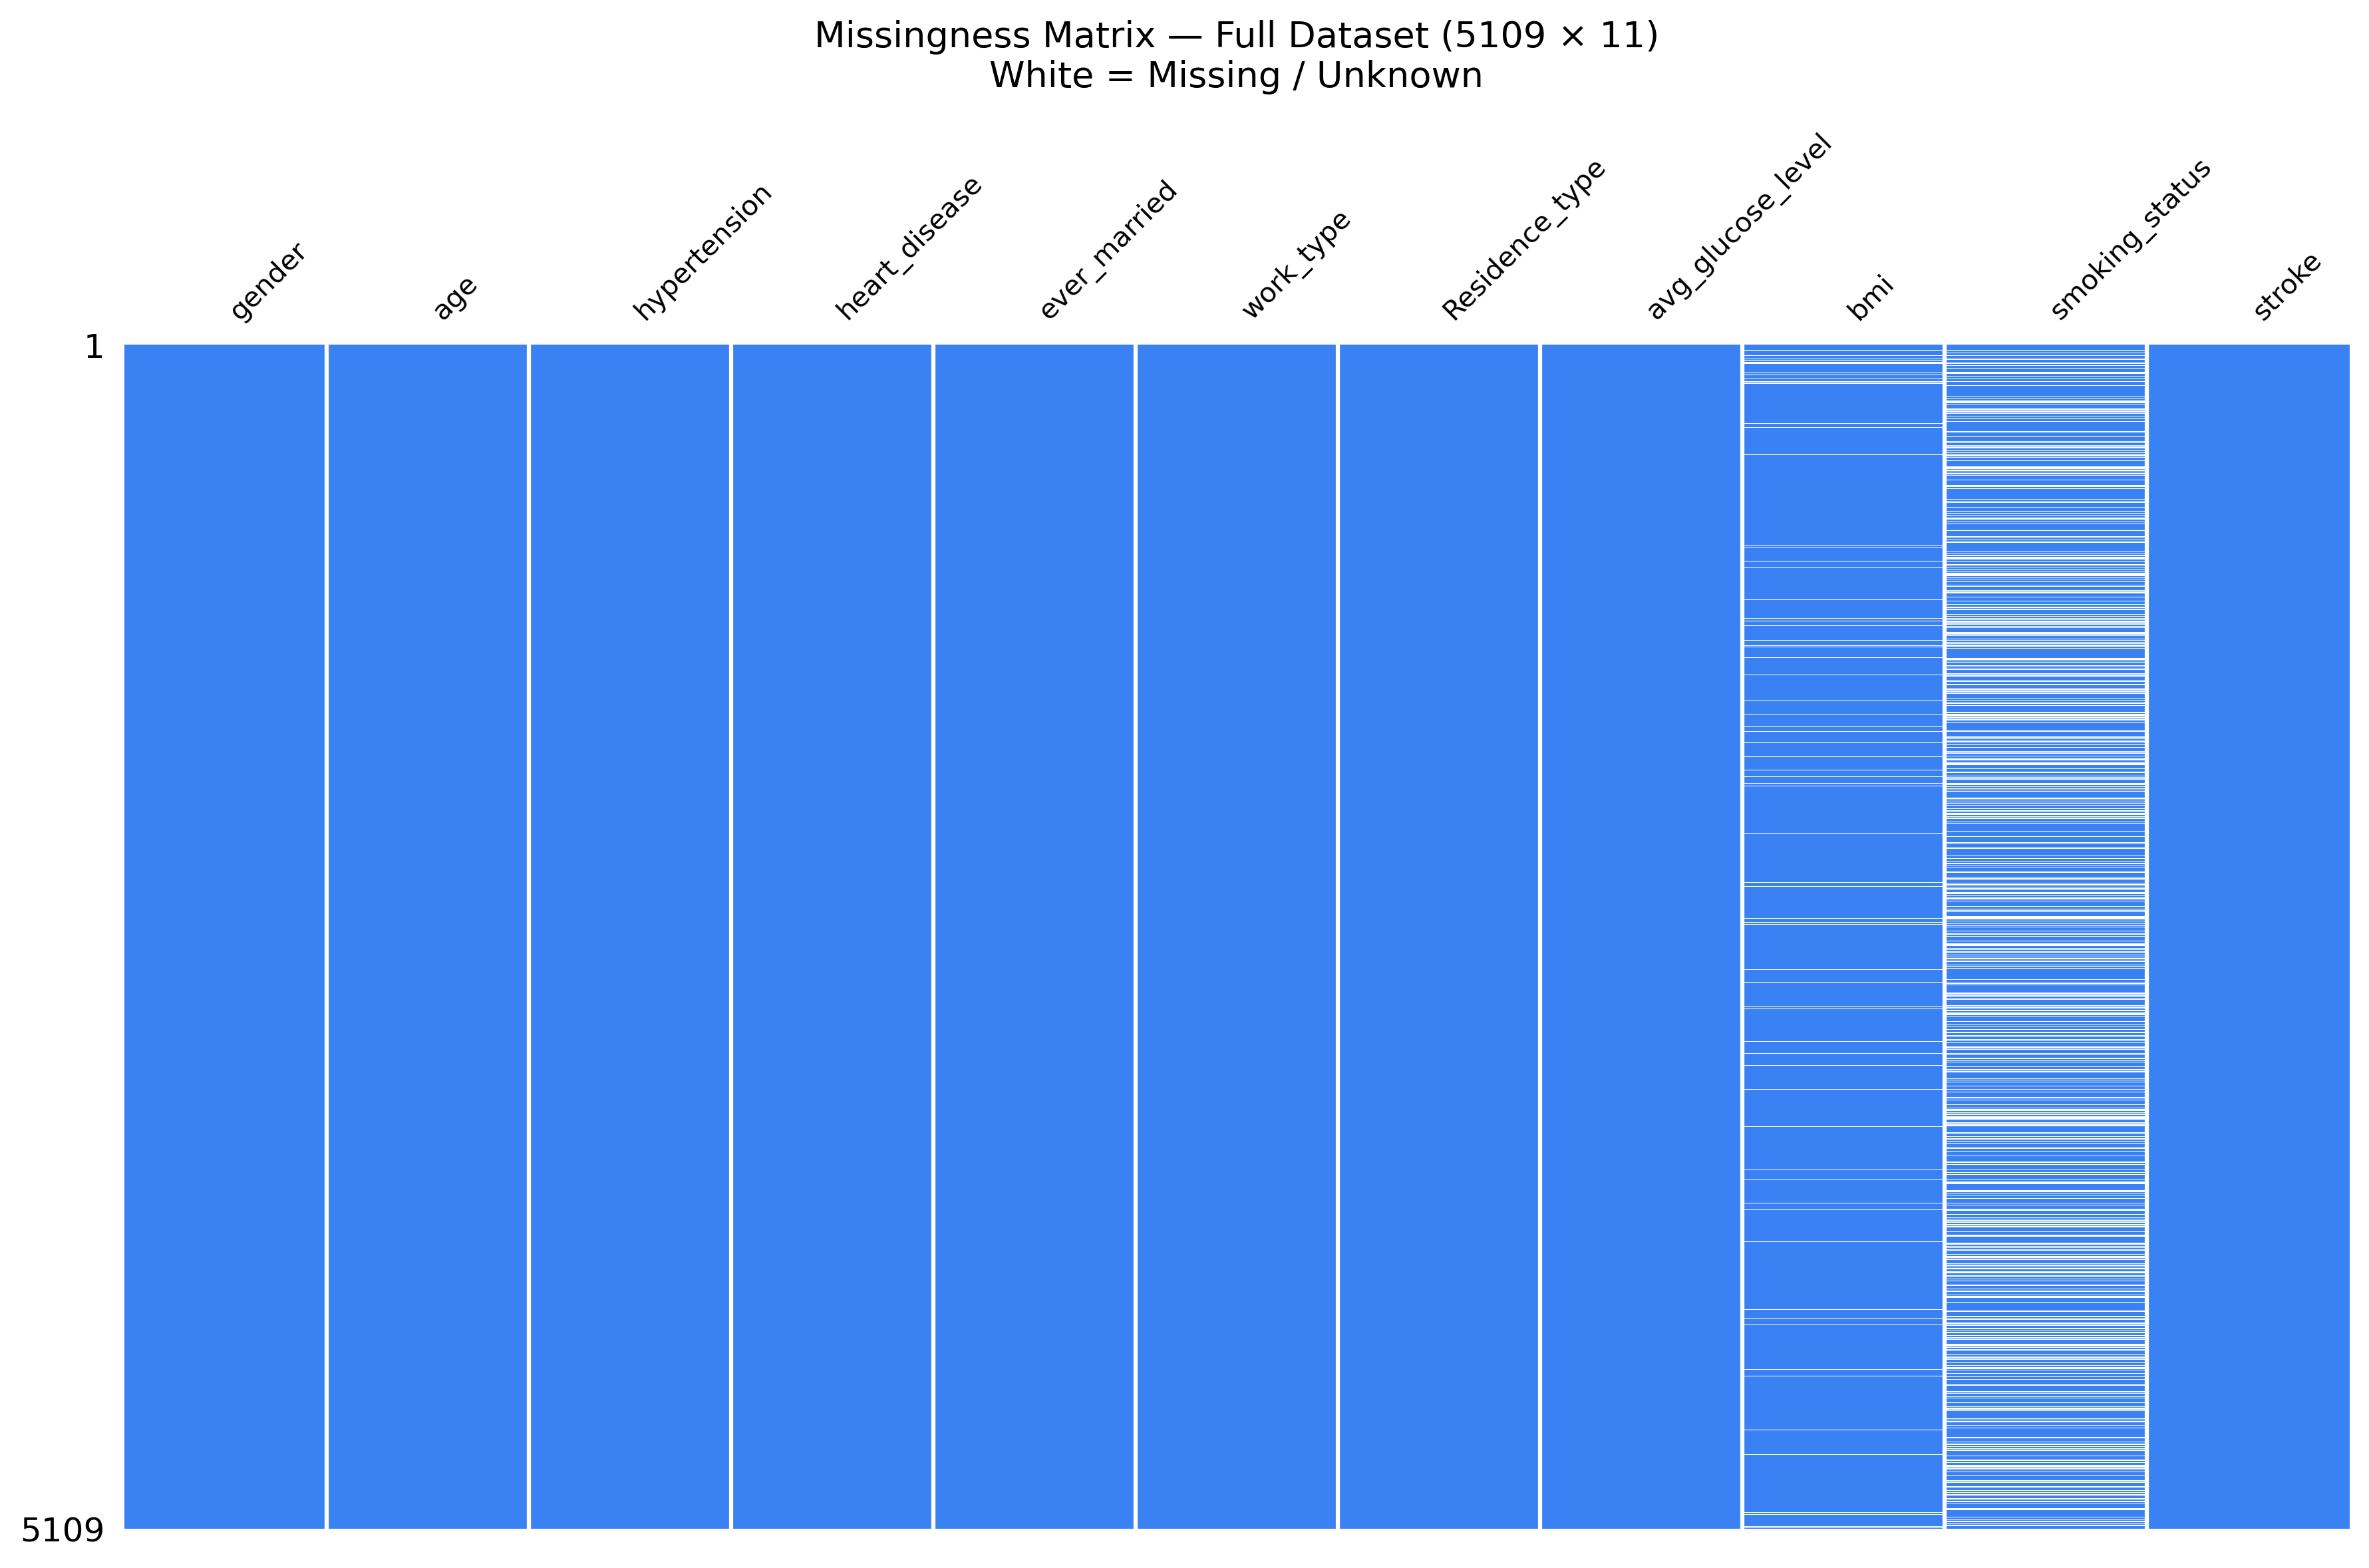
\includegraphics[width=\linewidth]{04_missing_data_audit.png}
    \caption{Missing data audit.}
    \label{fig:missing}
  \end{subfigure}
  \caption{Feature correlation (left) and missingness profile (right).}
\end{figure}

Two features have missing values:
\begin{itemize}
  \item \texttt{smoking\_status}: 1{,}544 entries ($30.2\%$) labelled ``Unknown'' — these are retained as a distinct category and an indicator variable \texttt{smoking\_unknown} is created.
  \item \texttt{bmi}: 201 missing values ($3.9\%$) — imputed by median; an additional binary flag \texttt{bmi\_missing} is added because the missingness indicator itself is a significant predictor ($\chi^{2}=98.56$, $p=3.16\times10^{-23}$: stroke rate $19.9\%$ when missing vs.\ $4.3\%$ when observed).
\end{itemize}

% -------------------------------------------------------
\subsection{Dataset Preprocessing}
% -------------------------------------------------------

\subsubsection{Train / Test Split}

The dataset is divided into an 80\% training set and a 20\% held-out test set using \emph{stratified} random sampling to preserve the class ratio in both splits.
This yields approximately 4{,}088 training samples (200 positive) and 1{,}022 test samples (49 positive).
All preprocessing is fitted exclusively on the training set to prevent data leakage.

\paragraph{Reproducibility and seeds.}
A global seed \texttt{SEED\,=\,42} (defined in \texttt{code/shared.py}) is applied uniformly: it is passed as \texttt{random\_state=42} to \texttt{train\_test\_split}, \texttt{StratifiedKFold}, all scikit-learn model constructors, and all resampling objects.
For the PyTorch MLP the seed block below is executed before each training run:
{\small\begin{verbatim}
  torch.manual_seed(42)
  torch.cuda.manual_seed_all(42)
  torch.backends.cudnn.deterministic = True
  torch.backends.cudnn.benchmark     = False
\end{verbatim}}
Running any script with these settings on the same hardware reproduces the exact results reported.

\subsubsection{Preprocessing Pipeline}

A \texttt{ColumnTransformer} applies the following transformations in parallel:

\begin{enumerate}
  \item \textbf{Numeric block} (\texttt{age}, \texttt{avg\_glucose\_level}, \texttt{bmi}):
        \begin{itemize}
          \item Median imputation (\texttt{SimpleImputer(strategy=``median'')}).
          \item Standardisation (\texttt{StandardScaler}).
        \end{itemize}
  \item \textbf{Categorical block} (\texttt{gender}, \texttt{ever\_married}, \texttt{work\_type}, \texttt{Residence\_type},\linebreak \texttt{smoking\_status}):
        \begin{itemize}
          \item One-hot encoding (\texttt{OneHotEncoder(handle\_unknown=``ignore'')}).
        \end{itemize}
  \item \textbf{Passthrough block} (\texttt{hypertension}, \texttt{heart\_disease}, \texttt{bmi\_missing}):
        \begin{itemize}
          \item Passed through unchanged (already binary 0/1).
        \end{itemize}
\end{enumerate}

The encoded feature space contains approximately 25 dimensions after one-hot expansion.

\subsubsection{Imbalance Handling}

Oversampling (SMOTE, ADASYN) is applied \emph{after} the preprocessor and \emph{only} on the training fold within each cross-validation split.
This is enforced by wrapping the entire sequence — imputer $\to$ scaler / encoder $\to$ resampler $\to$ classifier — inside a single \texttt{imblearn.pipeline.Pipeline}.
Because scikit-learn calls \texttt{fit} on each pipeline stage sequentially and only on the current training fold, \textbf{no information from the validation or test fold ever touches the fitted preprocessor or the synthetic samples}, eliminating both preprocessing leakage and oversampling leakage.
Class-weight arguments are passed directly to model constructors and require no additional safeguards.

\subsubsection{Cross-Validation}

{\tolerance=1500 All hyperparameter selection and experiment comparisons use 5-fold Stratified Cross-Validation on the training set, preserving the minority-class ratio across folds.
\textbf{The held-out test set is evaluated exactly once} — after the best pipeline is selected — and is never used to inform any modelling decision.}

% ============================================================
\section{Coding Environment}
\label{sec:env}
% ============================================================

\begin{table}[H]
  \centering
  \caption{Tools, libraries, and frameworks used (versions reflect the execution environment).}
  \label{tab:environment}
  \begin{tabular}{llll}
    \toprule
    \textbf{Category} & \textbf{Tool / Library} & \textbf{Version} & \textbf{Purpose} \\
    \midrule
    Language       & Python          & 3.12.7  & Core programming language \\
    Data           & pandas          & 2.3.3   & Data manipulation \\
    Data           & NumPy           & 2.0.2   & Numerical computing \\
    ML framework   & scikit-learn    & 1.8.0   & Classical models, pipelines, evaluation \\
    Imbalance      & imbalanced-learn & 0.14.1 & SMOTE, ADASYN, under-sampling \\
    Boosting       & XGBoost         & 3.2.0   & Gradient-boosted trees \\
    Deep learning  & PyTorch         & 2.9.1   & MLP implementation \\
    Explainability & SHAP            & 0.51.0  & Global \& local feature attribution \\
    Explainability & LIME            & 0.2.0.1 & Local surrogate explanations \\
    Visualisation  & matplotlib      & 3.10.8  & Figures and plots \\
    Visualisation  & seaborn         & 0.13.2  & Statistical visualisations \\
    Version ctrl   & Git / GitHub    & —       & Code versioning (see below) \\
    \bottomrule
  \end{tabular}
\end{table}

\noindent\textbf{Repository and dataset.}
The full source code is publicly available at:
\begin{center}
  \url{https://github.com/umutcaginozcan/cs464-project}
\end{center}
The dataset used is the \textit{Healthcare Dataset Stroke Data} (version 1) published by F.\ Soriano on Kaggle~\cite{fedesoriano2021stroke}.

% ============================================================
\section{Details of the Trained Models}
\label{sec:models}
% ============================================================

\subsection{Classical Machine Learning Models}

\subsubsection{Logistic Regression}
Logistic Regression fits a linear decision boundary in feature space and outputs calibrated probability estimates via the sigmoid function:
\[
  P(y=1 \mid \mathbf{x}) = \frac{1}{1+e^{-(\mathbf{w}^\top\mathbf{x}+b)}}.
\]
It is well-suited to high-dimensional, sparse tabular data, produces natively interpretable coefficients, and supports $L_1$ / $L_2$ regularisation.
Key hyperparameters: regularisation strength $C$, penalty type (\texttt{l1}, \texttt{l2}), and \texttt{class\_weight}.

\subsubsection{Gaussian Naive Bayes}
GNB assumes feature independence and Gaussian marginals within each class.
Despite its strong independence assumption, GNB is computationally efficient, works well with small training sets, and has no hyperparameters to tune—useful as a probabilistic baseline.

\subsubsection{$k$-Nearest Neighbours}
KNN classifies a sample by majority vote of its $k$ nearest neighbours.
We evaluate $k \in \{1, 3, 5, 7, 9\}$.
KNN is sensitive to the class-imbalance problem because the majority class tends to dominate neighbourhoods; it benefits significantly from resampling.

\subsubsection{Support Vector Machine (RBF Kernel)}
SVM with a radial basis function (RBF) kernel maps inputs to a high-dimensional space and finds the maximum-margin hyperplane.
Key hyperparameters: $C$ (margin penalty) and $\gamma$ (RBF bandwidth).
The \texttt{class\_weight=``balanced''} option re-weights the hinge loss inversely proportional to class frequencies.

\subsubsection{Random Forest}
Random Forest aggregates predictions from $T$ decision trees, each trained on a bootstrap sample with random feature subsets.
Hyperparameters include the number of trees (\texttt{n\_estimators}), maximum tree depth (\texttt{max\_depth}), and minimum samples per leaf.
The ensemble reduces variance and provides feature importance estimates.

\subsubsection{XGBoost}
XGBoost builds trees sequentially, fitting each tree to the pseudo-residuals of the ensemble so far.
The parameter \texttt{scale\_pos\_weight} directly addresses class imbalance by upweighting the minority-class gradient.
Regularisation via \texttt{reg\_alpha} (L1) and \texttt{reg\_lambda} (L2) on leaf weights controls overfitting.
Key hyperparameters: \texttt{n\_estimators}, \texttt{max\_depth}, \texttt{learning\_rate}, \texttt{subsample}, \texttt{colsample\_bytree}, \texttt{scale\_pos\_weight}.

% -------------------------------------------------------
\subsection{Deep Learning: PyTorch MLP}
% -------------------------------------------------------

\subsubsection{Architecture}

We implement a fully connected MLP with two hidden layers:
\[
  \mathbf{x}
  \xrightarrow{\text{FC}_{d\to64}}
  \text{ReLU}
  \xrightarrow{\text{Dropout}(0.2)}
  \xrightarrow{\text{FC}_{64\to32}}
  \text{ReLU}
  \xrightarrow{\text{Dropout}(0.2)}
  \xrightarrow{\text{FC}_{32\to1}}
  \hat{y}_{\text{logit}},
\]
where $d \approx 25$ is the preprocessed feature dimension.
Dropout prevents overfitting on the small training set.

\subsubsection{Loss Functions}

Three training configurations are compared:

\begin{enumerate}
  \item \textbf{Binary Cross-Entropy (BCE):}
        $\mathcal{L}_{\text{BCE}} = -[y\log\hat{p} + (1-y)\log(1-\hat{p})]$.
        No imbalance correction—serves as a deep-learning baseline.

  \item \textbf{Weighted BCE:}
        $\mathcal{L}_{\text{wBCE}} = -[w_+ y\log\hat{p} + (1-y)\log(1-\hat{p})]$,
        where $w_+ = N_{\text{neg}}/N_{\text{pos}} \approx 19.5$.
        Upweights minority-class prediction errors.

  \item \textbf{Focal Loss~\cite{lin2017focal}:}
        $\mathcal{L}_{\text{focal}} = -(1-\hat{p})^\gamma \log\hat{p}$, with $\gamma=2$.
        Down-weights easy examples so the model focuses on hard, misclassified cases.
\end{enumerate}

\subsubsection{Training Configuration}

\begin{itemize}
  \item Optimiser: Adam with learning rate $10^{-3}$.
  \item Batch size: 64.
  \item Maximum epochs: 100 with early stopping (patience 10) monitored on validation AUC-PR.
  \item Data split: the training set is further divided 80/20 into train/validation splits (stratified).
\end{itemize}

% ============================================================
\section{Experimental Setup}
\label{sec:experiments}
% ============================================================

All experiments follow the same evaluation protocol: metrics are reported for the held-out test set (Table~\ref{tab:exp_summary}).
For classical models, a 5-fold stratified CV is used to guide model selection, and the test set is evaluated exactly once per configuration.

\begin{table}[H]
  \centering
  \caption{Summary of experimental phases.}
  \label{tab:exp_summary}
  \renewcommand{\arraystretch}{1.1}
  \begin{tabular}{clll}
    \toprule
    \textbf{ID} & \textbf{Experiment} & \textbf{Purpose} & \textbf{Models} \\
    \midrule
    0 & Baseline               & Expose accuracy paradox        & All 10 \\
    1 & Class Weighting        & Cost-sensitive loss             & LR, SVM, XGB \\
    2 & SMOTE                  & Synthetic oversampling          & LR, SVM, XGB, KNN \\
    3 & ADASYN                 & Adaptive oversampling           & LR, SVM, XGB \\
    4 & Threshold Tuning       & Post-hoc decision boundary      & Best from Exp.\ 0–3 \\
    H & Hyperparameter Search  & Joint pipeline optimisation     & LR, SVM, RF, XGB \\
    DL & Deep Learning (MLP)   & Neural network comparison       & MLP $\times$ 3 losses \\
    C & Calibration            & Post-hoc probability correction & Winner model \\
    \bottomrule
  \end{tabular}
\end{table}

\subsection{Experiment 0 — Baseline}

All ten models are trained with default scikit-learn hyperparameters and no imbalance correction.
This establishes the accuracy paradox as a starting point.

\subsection{Experiment 1 — Class Weighting}

Class weights are set to \texttt{``balanced''}, which sets $w_k \propto N/(K \cdot N_k)$.
For this dataset the minority-class weight is approximately $w_1 \approx 10.26$.
This modifies the loss function without altering the training data distribution.

\subsection{Experiment 2 — SMOTE}

SMOTE (Synthetic Minority Over-sampling Technique)~\cite{chawla2002smote} generates synthetic minority samples by linear interpolation between a minority sample $\mathbf{x}_i$ and one of its $k$-nearest minority neighbours $\mathbf{x}_j$:
\[
  \mathbf{x}_{\text{new}} = \mathbf{x}_i + \lambda(\mathbf{x}_j - \mathbf{x}_i), \quad \lambda \sim \mathcal{U}(0,1).
\]
Oversampling is performed on the training fold only, after preprocessing.

\subsection{Experiment 3 — ADASYN}

ADASYN~\cite{he2008adasyn} extends SMOTE with adaptive sampling: minority samples with more majority-class neighbours receive proportionally more synthetic samples.
The sampling density for sample $i$ is:
\[
  \hat{r}_i = \frac{\Gamma_i}{\sum_j \Gamma_j}, \quad
  \Gamma_i = \frac{|\{x_j \in \text{kNN}(x_i) : y_j = 0\}|}{k}.
\]
On this dataset, the $\Gamma_i$ distribution is nearly constant, so ADASYN produces results similar to SMOTE.

\subsection{Experiment 4 — Threshold Tuning}

Rather than retraining, we optimise the decision threshold $t$ post-hoc:
\[
  t^* = \arg\max_{t \in [0,1]} F_1(t).
\]
Three operating points are evaluated per model:
\begin{itemize}
  \item \textbf{Screening} ($\text{Recall} \geq 0.90$, maximise precision) — minimise missed strokes.
  \item \textbf{Balanced} ($t^*$, maximise $F_1$) — balance precision and recall.
  \item \textbf{Confirmatory} ($\text{Precision} \geq 0.30$, maximise recall) — confirm likely cases.
\end{itemize}

\subsection{Hyperparameter Search}

We perform a systematic joint search over 80 pipeline configurations:
$4\ \text{imputation strategies} \times 5\ \text{resampling strategies} \times 4\ \text{models}$.
Each configuration is scored by 5-fold CV AUC-PR.
The model hyperparameter search spaces are given in Table~\ref{tab:hpspace}.

\begin{table}[H]
  \centering
  \caption{Hyperparameter search spaces (randomised search, $n\_iter$ per model).}
  \label{tab:hpspace}
  \renewcommand{\arraystretch}{1.1}
  \begin{tabular}{lp{9cm}c}
    \toprule
    \textbf{Model} & \textbf{Hyperparameters} & \textbf{Iter.} \\
    \midrule
    Logistic Regression & $C \in \{0.001,0.01,0.1,1,10,100\}$; penalty $\in \{l_1,l_2\}$; \texttt{class\_weight} & 10 \\
    SVM (RBF) & $C \in \{0.1,1,10,100\}$; $\gamma \in \{\texttt{scale}, \texttt{auto}, 0.001, 0.01, 0.1\}$ & 10 \\
    Random Forest & \texttt{n\_estimators} $\in \{100,200,300\}$; \texttt{max\_depth}; \texttt{max\_features} & 15 \\
    XGBoost & \texttt{n\_estimators}, \texttt{max\_depth}, \texttt{learning\_rate}, \texttt{subsample}, \texttt{scale\_pos\_weight} & 20 \\
    \bottomrule
  \end{tabular}
\end{table}

\subsection{Threshold Tuning (Experiment 4)}

The optimal threshold $t^*$ is identified by sweeping over the out-of-fold predicted probabilities produced during 5-fold CV on the training set — \emph{not} on the test set.
This ensures $t^*$ is selected without any access to held-out labels, preserving the integrity of the final evaluation.

\subsection{Calibration}

To fit the calibrators without contaminating the test set, the training set is further split into:
\begin{itemize}
  \item \textbf{Fit set} ($80\%$ of training, $\approx\!3{,}270$ samples) — used to train the base model.
  \item \textbf{Calibration set} ($20\%$ of training, $\approx\!818$ samples) — held out and used exclusively to fit the Platt / isotonic calibrator on the base model's raw probability outputs.
\end{itemize}
The calibrated model is then evaluated on the original held-out test set.
We apply two post-hoc calibration methods:
\begin{itemize}
  \item \textbf{Platt scaling} — fits a logistic regression on the calibration-set scores.
  \item \textbf{Isotonic regression} — fits a non-parametric monotone function on the calibration-set scores.
\end{itemize}
Calibration quality is measured by the Brier score $\text{BS} = \frac{1}{N}\sum_i(\hat{p}_i - y_i)^2$ and reliability diagrams.

% ============================================================
\section{Results \& Discussion}
\label{sec:results}
% ============================================================

\subsection{Baseline Results (Experiment 0)}

Table~\ref{tab:baseline} shows that all models achieve high accuracy ($>\!90\%$) but catastrophically low recall ($0$–$4\%$) on the stroke class.
This is the accuracy paradox: the models learn to ignore the minority class entirely.

\begin{table}[H]
  \centering
  \caption{Experiment 0 — Baseline test-set performance (no imbalance correction).}
  \label{tab:baseline}
  \renewcommand{\arraystretch}{1.1}
  \begin{tabular}{lcccccc}
    \toprule
    \textbf{Model} & \textbf{Acc.} & \textbf{Recall} & \textbf{Prec.} & \textbf{F1} & \textbf{AUC-ROC} & \textbf{AUC-PR} \\
    \midrule
    Logistic Regression  & 95.21\% & 2.00\%  & 100.00\% & 0.039 & 0.845 & 0.267 \\
    Gaussian NB          & 31.12\% & 98.00\% &   6.52\% & 0.122 & 0.789 & 0.159 \\
    KNN ($k=1$)          & 91.88\% &  4.00\% &   5.41\% & 0.046 & 0.560 & 0.049 \\
    KNN ($k=3$)          & 94.42\% &  4.00\% &  18.18\% & 0.066 & 0.528 & 0.057 \\
    KNN ($k=5$)          & 94.91\% &  0.00\% &   0.00\% & 0.000 & 0.591 & 0.065 \\
    KNN ($k=7$)          & 95.01\% &  0.00\% &   0.00\% & 0.000 & 0.626 & 0.077 \\
    KNN ($k=9$)          & 95.01\% &  0.00\% &   0.00\% & 0.000 & 0.661 & 0.087 \\
    SVM (RBF)            & 95.11\% &  0.00\% &   0.00\% & 0.000 & 0.678 & 0.114 \\
    Random Forest        & 95.01\% &  2.00\% &  33.33\% & 0.038 & 0.779 & 0.156 \\
    XGBoost              & 93.84\% &  4.00\% &  11.76\% & 0.060 & 0.787 & 0.146 \\
    \bottomrule
  \end{tabular}
\end{table}

\noindent\textit{Key observation:} Despite AUC-ROC scores in the $0.78$–$0.85$ range, F1 scores are near zero because models predict the majority class almost exclusively.
This confirms that AUC-ROC alone is misleading for severely imbalanced problems.

\subsection{Effect of Imbalance Handling (Experiments 1–3)}

Table~\ref{tab:imbalance} summarises the best results from each imbalance strategy.

\begin{table}[H]
  \centering
  \caption{Best test-set results per imbalance strategy. Best F1 per experiment shown in \textbf{bold}.}
  \label{tab:imbalance}
  \renewcommand{\arraystretch}{1.15}
  \begin{tabular}{llccccc}
    \toprule
    \textbf{Exp.} & \textbf{Best Model} & \textbf{Acc.} & \textbf{Recall} & \textbf{Prec.} & \textbf{F1} & \textbf{AUC-PR} \\
    \midrule
    \multirow{3}{*}{1 (Class Weight)} & LR  & 75.83\% & 80.00\% & 14.44\% & \textbf{0.245} & 0.261 \\
                                       & SVM & 78.38\% & 68.00\% & 14.23\% & 0.235 & 0.177 \\
                                       & XGB & 93.35\% & 10.00\% & 17.86\% & 0.128 & 0.170 \\
    \midrule
    \multirow{2}{*}{2 (SMOTE)}        & LR  & 75.73\% & 78.00\% & 14.13\% & \textbf{0.239} & 0.267 \\
                                       & SVM & 83.37\% & 46.00\% & 13.86\% & 0.213 & 0.167 \\
    \midrule
    \multirow{2}{*}{3 (ADASYN)}       & LR  & 75.34\% & 78.00\% & 13.93\% & \textbf{0.236} & 0.265 \\
                                       & XGB & 93.05\% & 14.00\% & 20.00\% & 0.165 & 0.174 \\
    \bottomrule
  \end{tabular}
\end{table}

\textbf{Discussion.}
Class weighting is the most effective single intervention: LR recall jumps from $2\%$ to $80\%$ (Exp.\ 0 $\to$ Exp.\ 1).
SMOTE produces similar recall to class weighting for LR but improves SVM considerably (from $0\%$ to $46\%$).
ADASYN yields results nearly identical to SMOTE, consistent with our observation that the $\Gamma_i$ distribution is nearly uniform for this dataset.
XGBoost consistently underperforms LR on recall under these strategies, likely because its ensemble structure is less responsive to cost-sensitive modifications without joint hyperparameter tuning.

\subsection{Deep Learning Results}

Table~\ref{tab:dl} shows MLP results under the three loss functions.

\begin{table}[H]
  \centering
  \caption{Deep Learning (PyTorch MLP) test-set performance.}
  \label{tab:dl}
  \renewcommand{\arraystretch}{1.1}
  \begin{tabular}{lccccc}
    \toprule
    \textbf{Loss Function} & \textbf{Acc.} & \textbf{Recall} & \textbf{Prec.} & \textbf{F1} & \textbf{AUC-PR} \\
    \midrule
    BCE (standard)       & 95.11\% & 0.00\% & 0.00\% & 0.000 & 0.236 \\
    Weighted BCE         & 74.56\% & 78.00\% & 13.54\% & \textbf{0.231} & 0.269 \\
    Focal Loss ($\gamma=2$) & 95.11\% & 0.00\% & 0.00\% & 0.000 & 0.243 \\
    \bottomrule
  \end{tabular}
\end{table}

\begin{figure}[H]
  \centering
  \begin{subfigure}[b]{0.32\linewidth}
    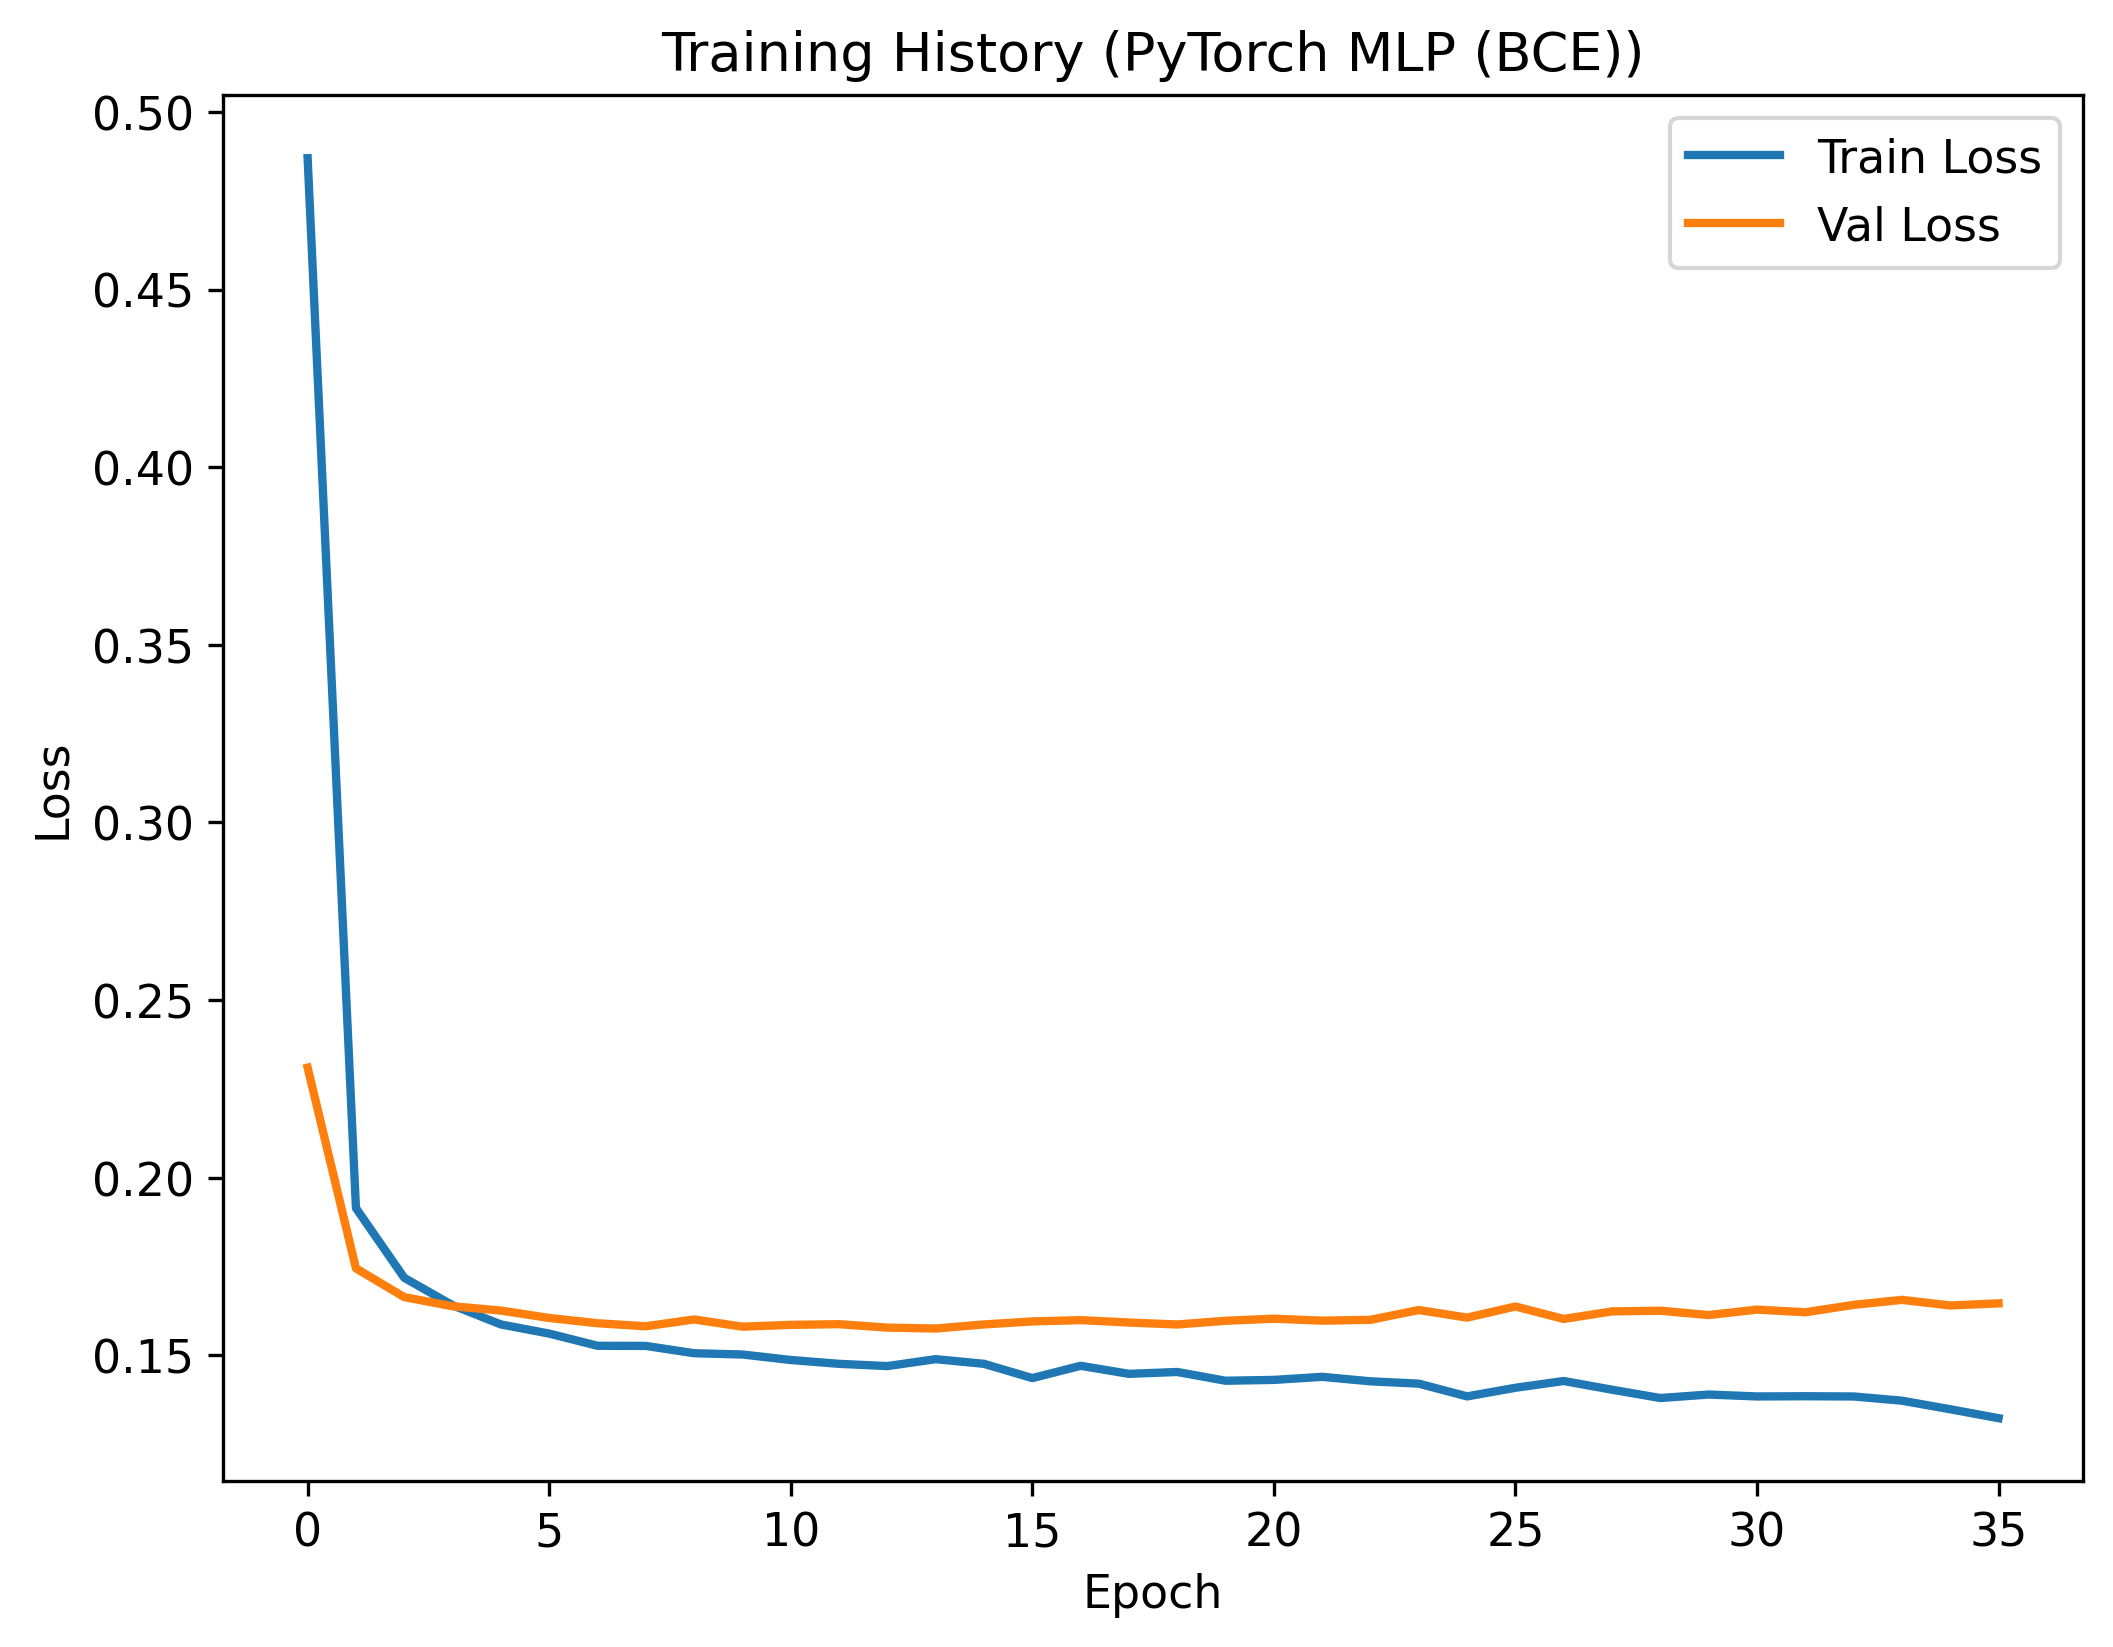
\includegraphics[width=\linewidth]{dl_mlp_training_history_bce.png}
    \caption{BCE loss.}
  \end{subfigure}
  \hfill
  \begin{subfigure}[b]{0.32\linewidth}
    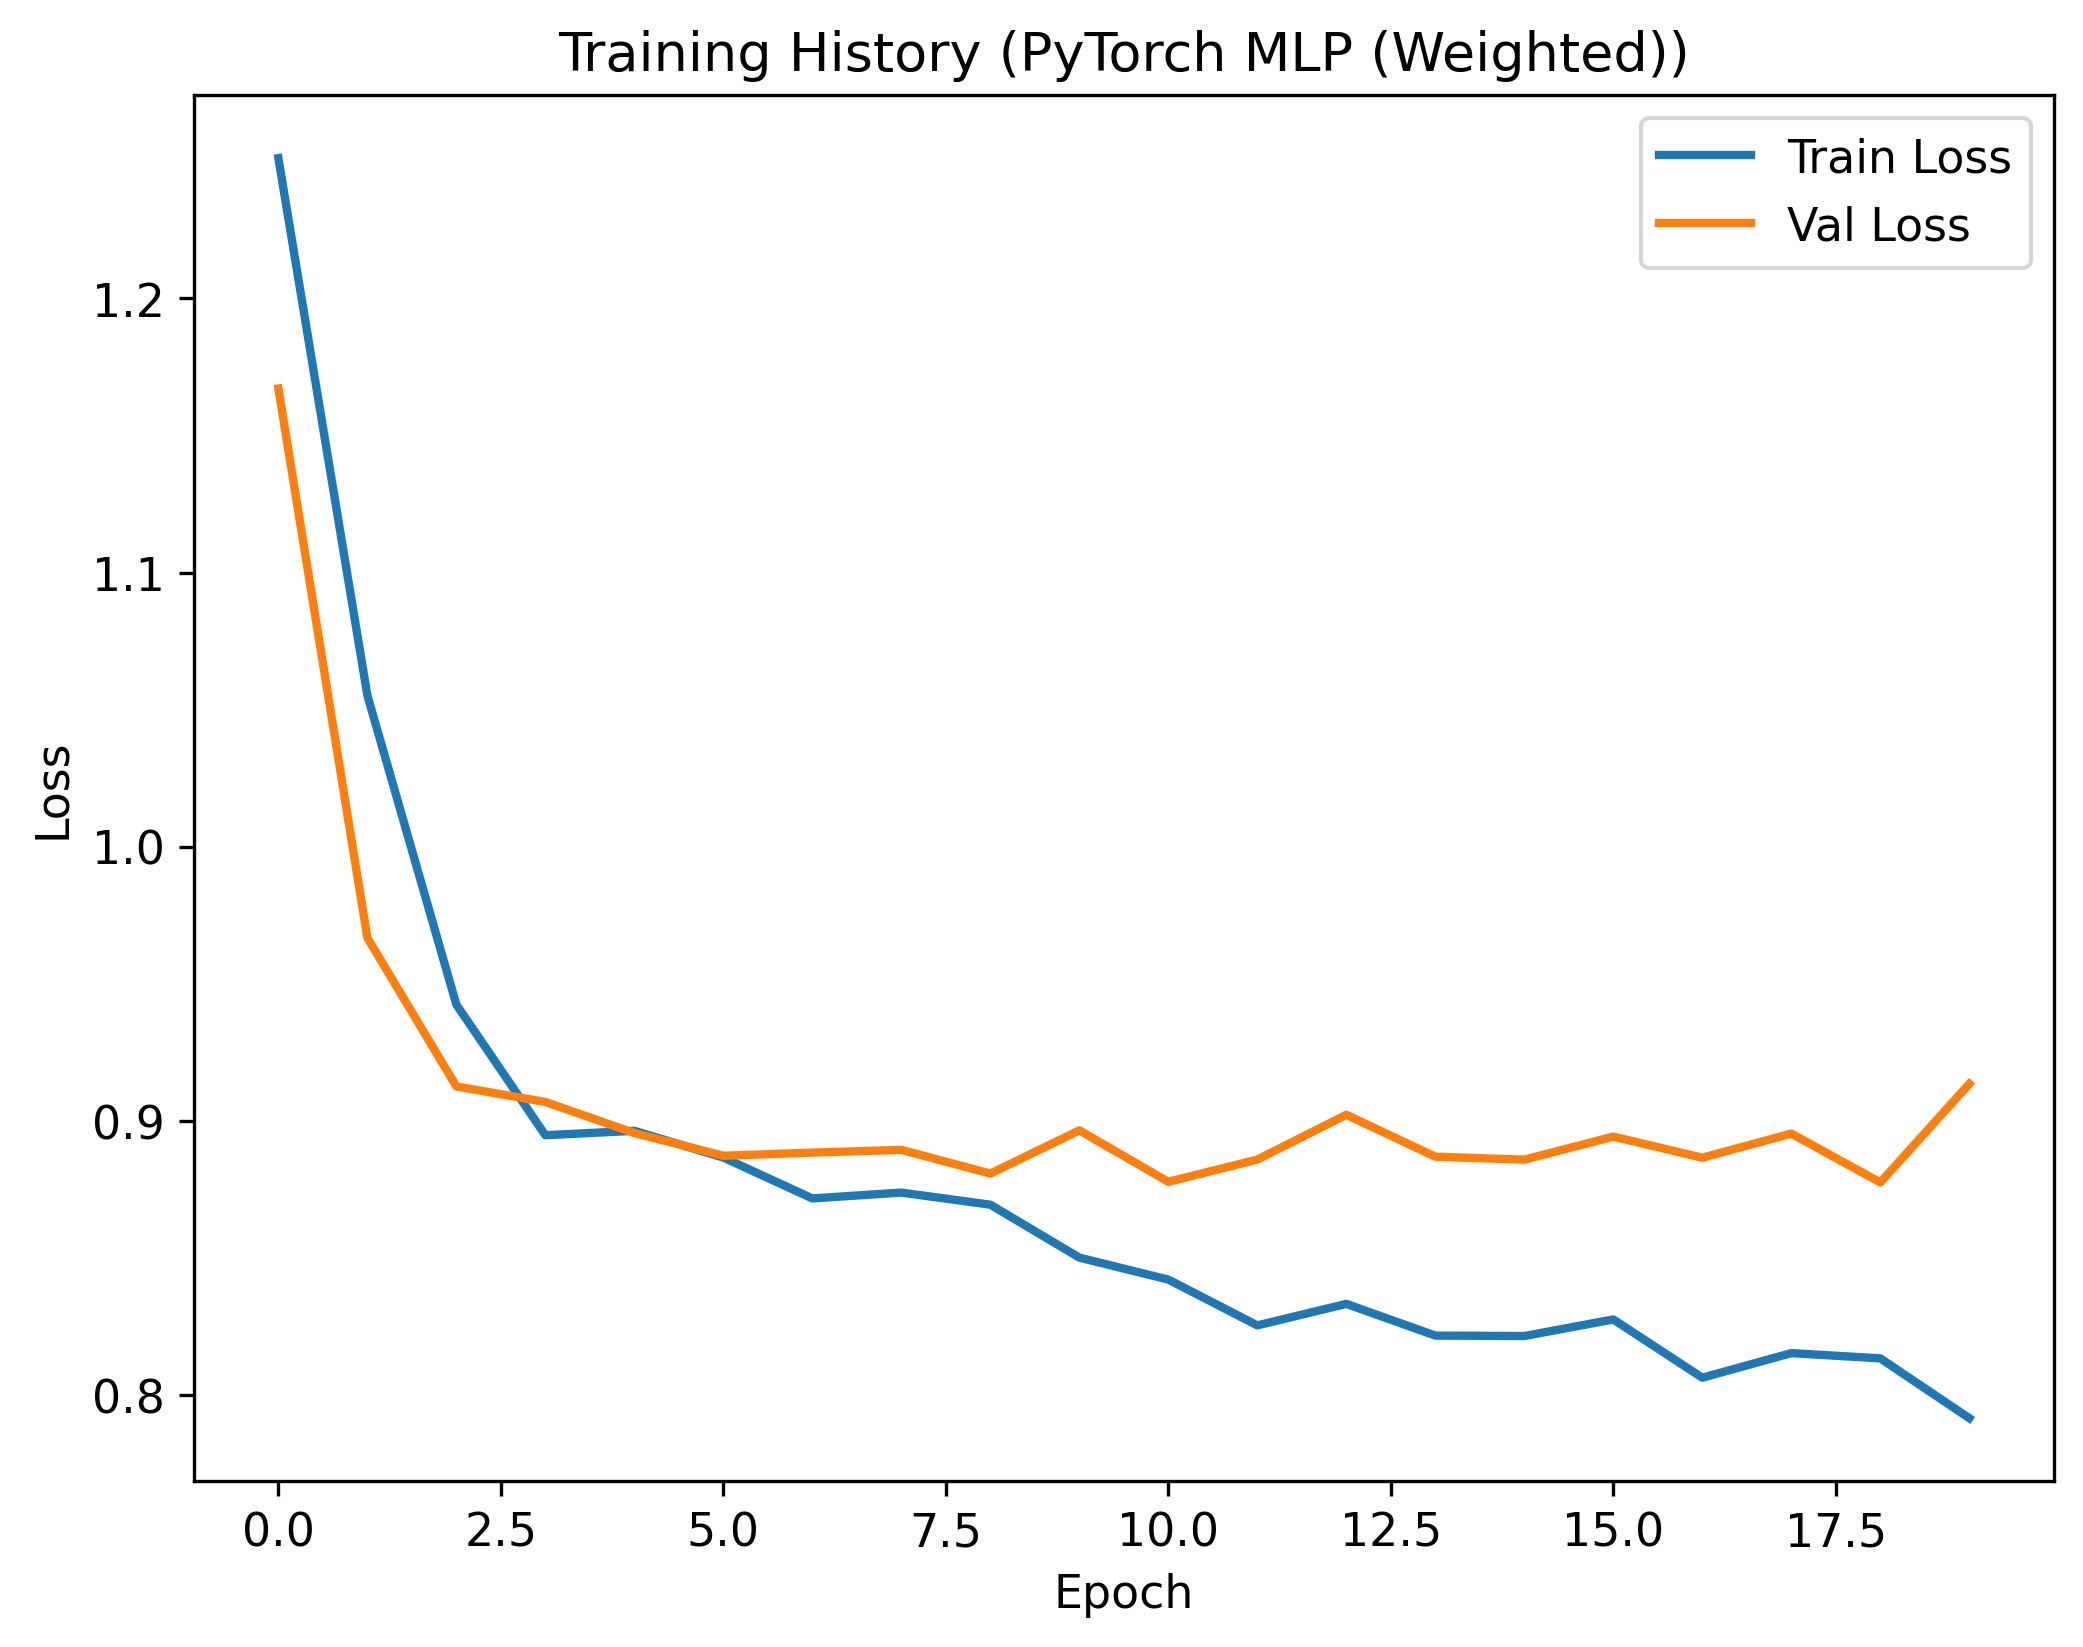
\includegraphics[width=\linewidth]{dl_mlp_training_history_weighted.png}
    \caption{Weighted BCE.}
  \end{subfigure}
  \hfill
  \begin{subfigure}[b]{0.32\linewidth}
    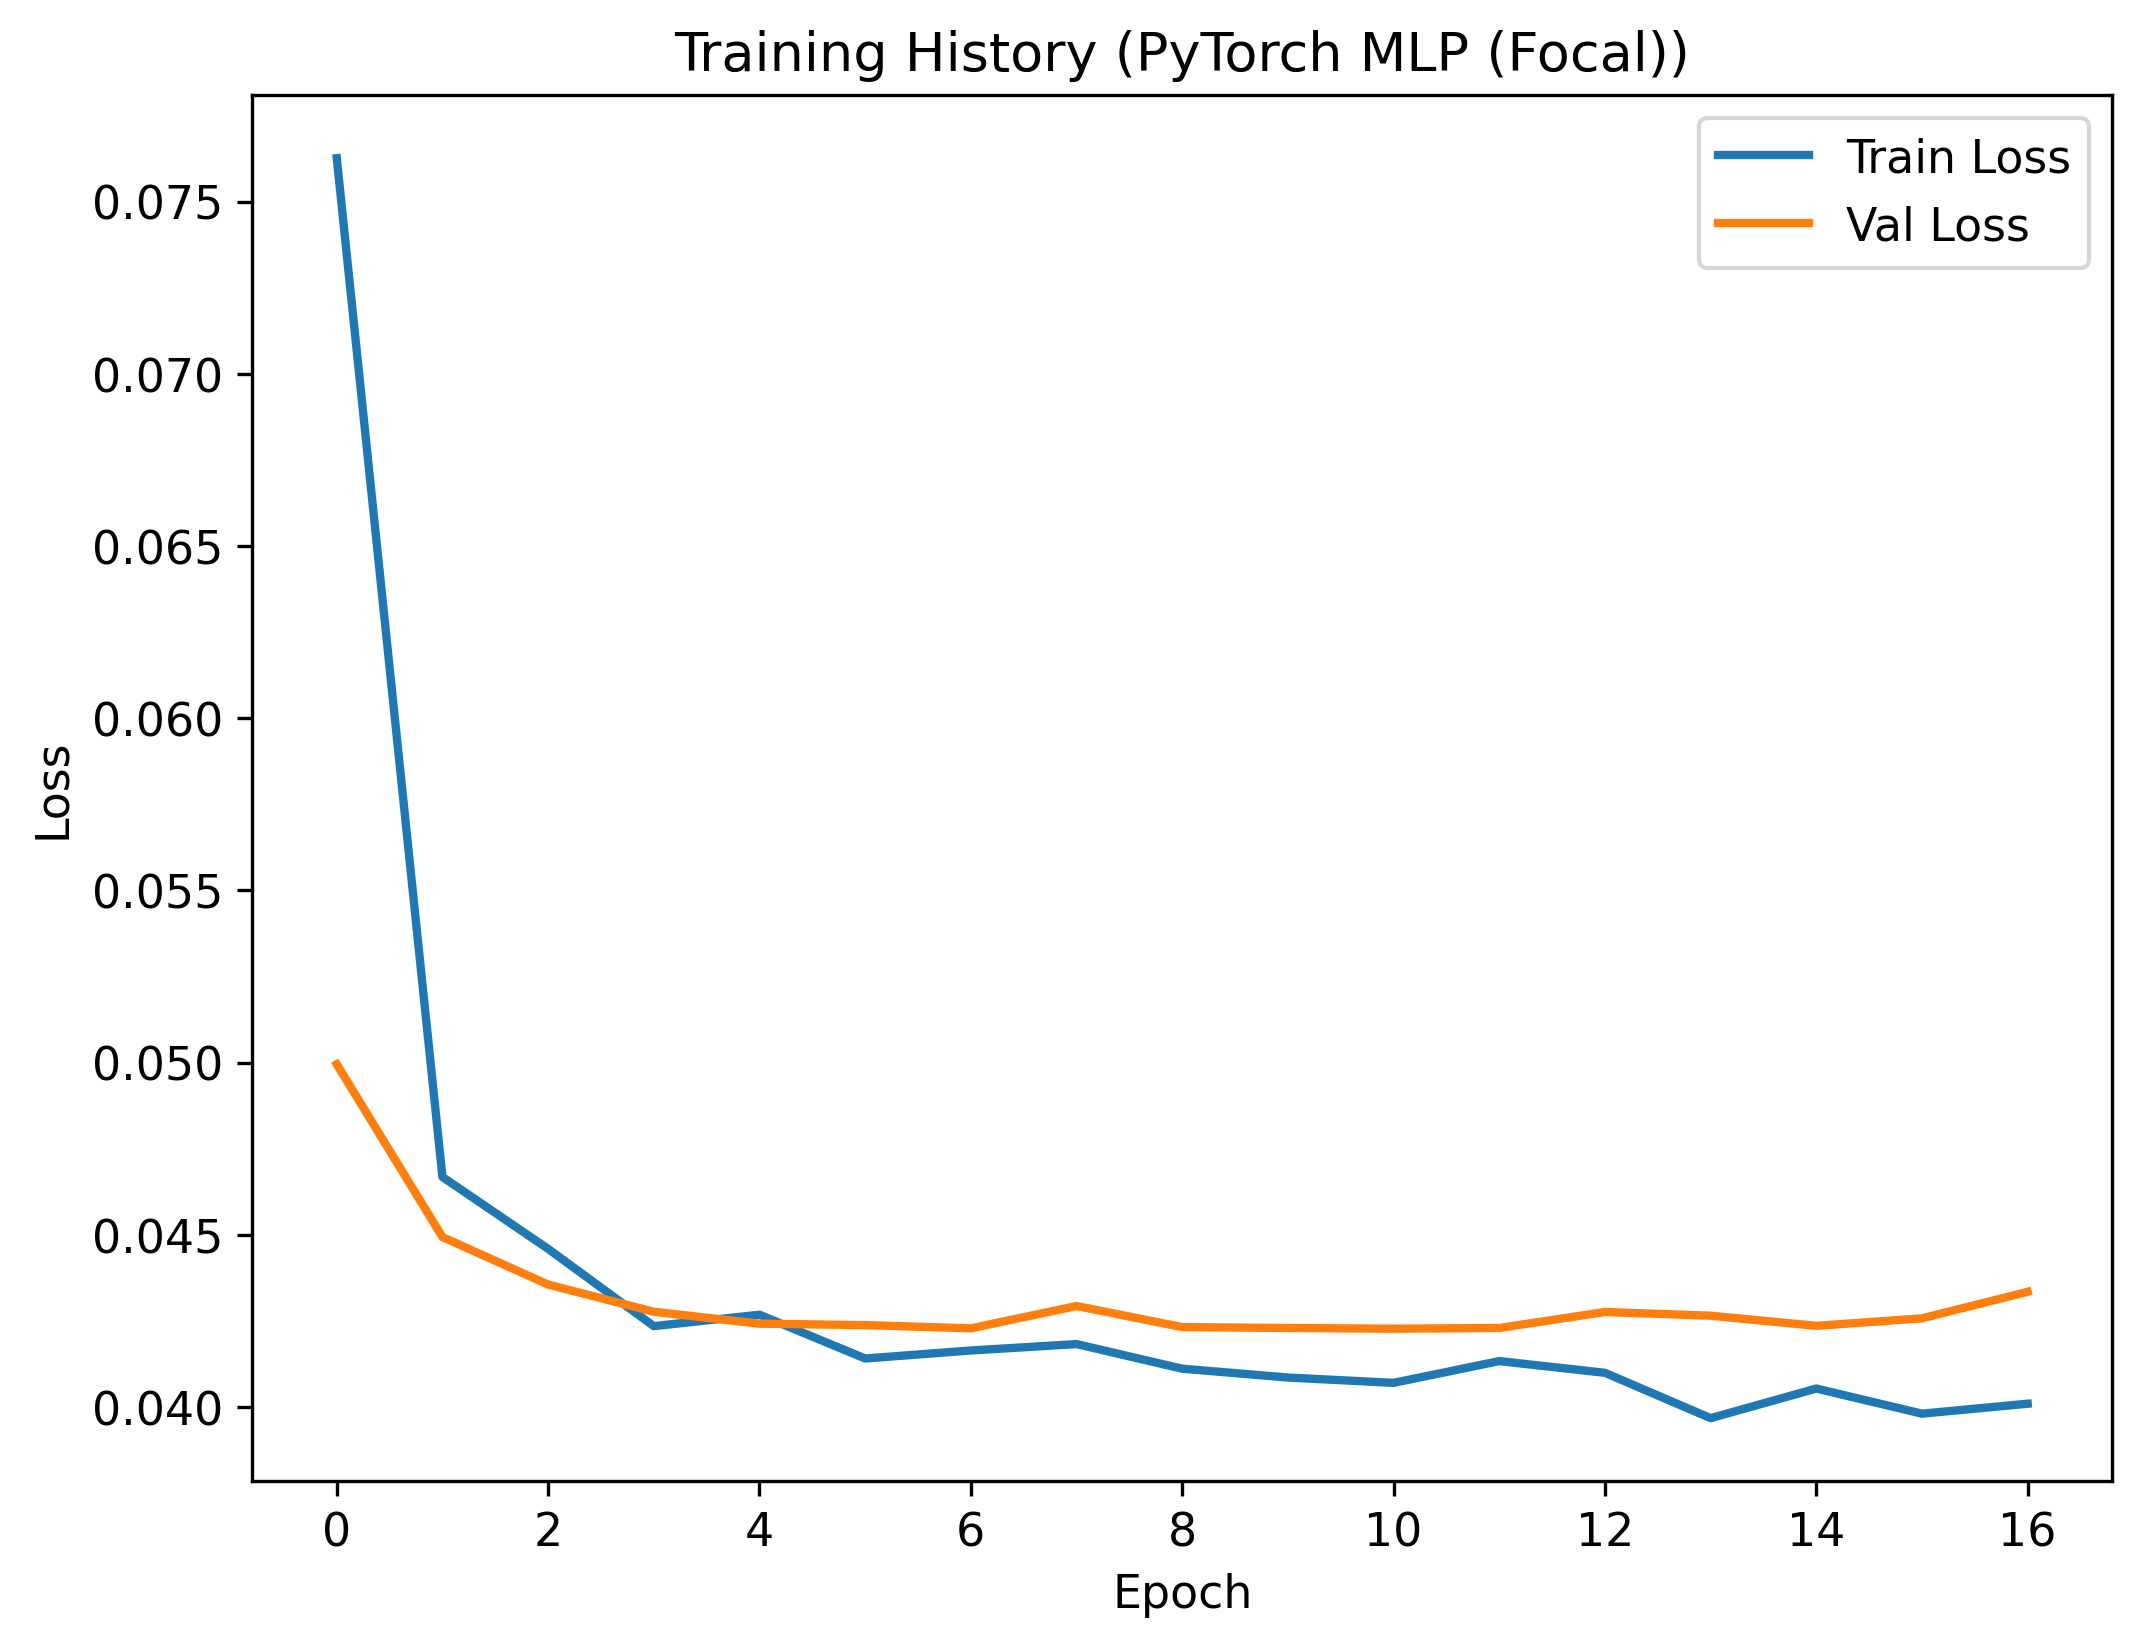
\includegraphics[width=\linewidth]{dl_mlp_training_history_focal.png}
    \caption{Focal Loss.}
  \end{subfigure}
  \caption{MLP training and validation curves for each loss function.}
  \label{fig:dl_curves}
\end{figure}

\textbf{Discussion.}
Standard BCE and Focal Loss both collapse to the majority class (recall $= 0$), producing near-perfect accuracy but zero stroke detection.
Despite the theoretical motivation of Focal Loss to emphasise hard examples, it does not suffice on its own for such severe imbalance.
Only Weighted BCE successfully breaks the majority-class collapse, matching classical LR performance (F1 $=0.231$, Recall $=78\%$).
This underscores that, for tabular data at this scale ($n\approx4{,}000$ training samples), a well-regularised linear model with cost-sensitive training is competitive with deep learning.

\subsection{Hyperparameter Search Results}

Table~\ref{tab:hyper} reports the best pipeline configuration per model family.

\begin{table}[H]
  \centering
  \caption{Best hyperparameter-tuned configurations (5-fold CV AUC-PR used for selection).}
  \label{tab:hyper}
  \renewcommand{\arraystretch}{1.1}
  \begin{tabular}{llccccc}
    \toprule
    \textbf{Model} & \textbf{Best Pipeline} & \textbf{Acc.} & \textbf{Recall} & \textbf{Prec.} & \textbf{F1} & \textbf{AUC-PR} \\
    \midrule
    \textbf{LR}  & median + undersample & 73.48\% & 82.00\% & 13.53\% & \textbf{0.232} & \textbf{0.300} \\
    SVM          & knn + smote          & 74.46\% & 78.00\% & 13.49\% & 0.230 & 0.282 \\
    RF           & knn + undersample    & 69.57\% & 82.00\% & 11.95\% & 0.209 & 0.242 \\
    XGBoost      & iterative + none     & 92.95\% & 28.00\% & 28.00\% & 0.280 & 0.266 \\
    \bottomrule
  \end{tabular}
\end{table}

\textbf{Winner model selection.}
Logistic Regression achieves the highest AUC-PR ($0.300$) among all tested configurations, making it the winner model on our primary metric.
While XGBoost achieves the highest F1 ($0.280$), its AUC-PR ($0.266$) is lower and its high accuracy ($92.95\%$) masks low recall ($28\%$), suggesting it errs toward precision.
For a clinical screening tool, high recall (catching stroke cases) is preferred, making LR the more suitable choice.

\subsection{Winner Model Analysis}

\subsubsection{Performance Summary}

\begin{table}[H]
  \centering
  \caption{Winner model (Logistic Regression, Tuned) — full test-set metrics.}
  \label{tab:winner}
  \begin{tabular}{lc}
    \toprule
    \textbf{Metric} & \textbf{Value} \\
    \midrule
    Accuracy        & 73.48\% \\
    Precision       & 13.53\% \\
    Recall          & 82.00\% \\
    F1 Score        & 0.2323 \\
    F2 Score        & 0.4076 \\
    AUC-ROC         & 0.8426 \\
    AUC-PR          & \textbf{0.3000} \\
    Brier Score     & 0.1689 \\
    \bottomrule
  \end{tabular}
\end{table}

\begin{figure}[H]
  \centering
  \begin{subfigure}[b]{0.48\linewidth}
    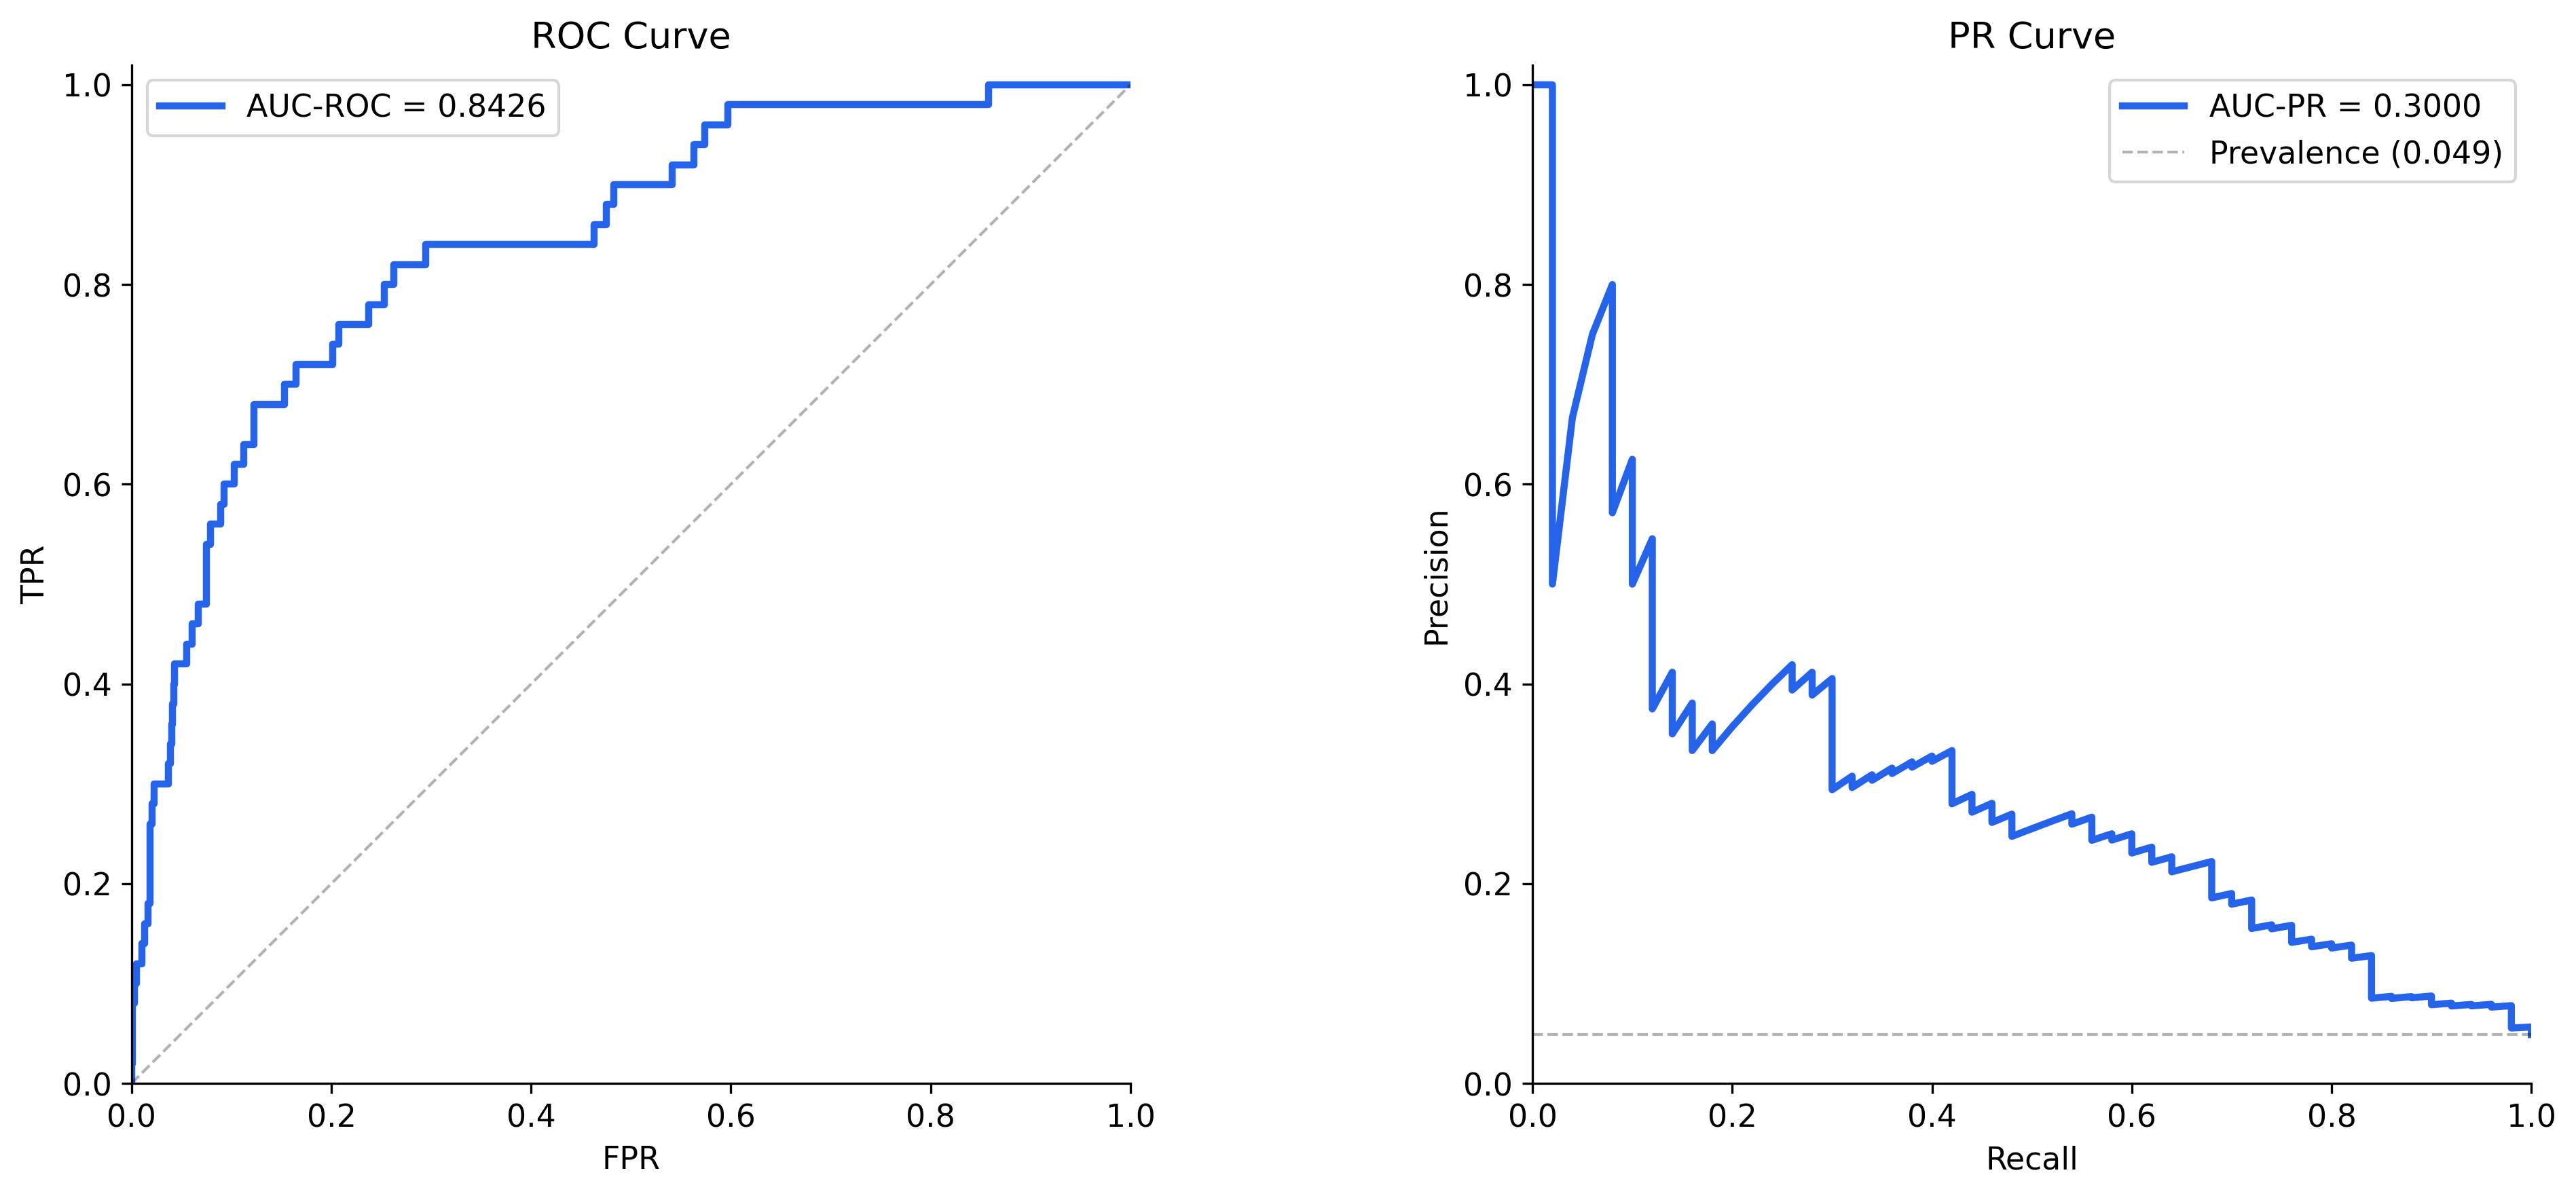
\includegraphics[width=\linewidth]{winner_analysis/roc_pr_curves.png}
    \caption{ROC and Precision-Recall curves.}
    \label{fig:roc_pr}
  \end{subfigure}
  \hfill
  \begin{subfigure}[b]{0.48\linewidth}
    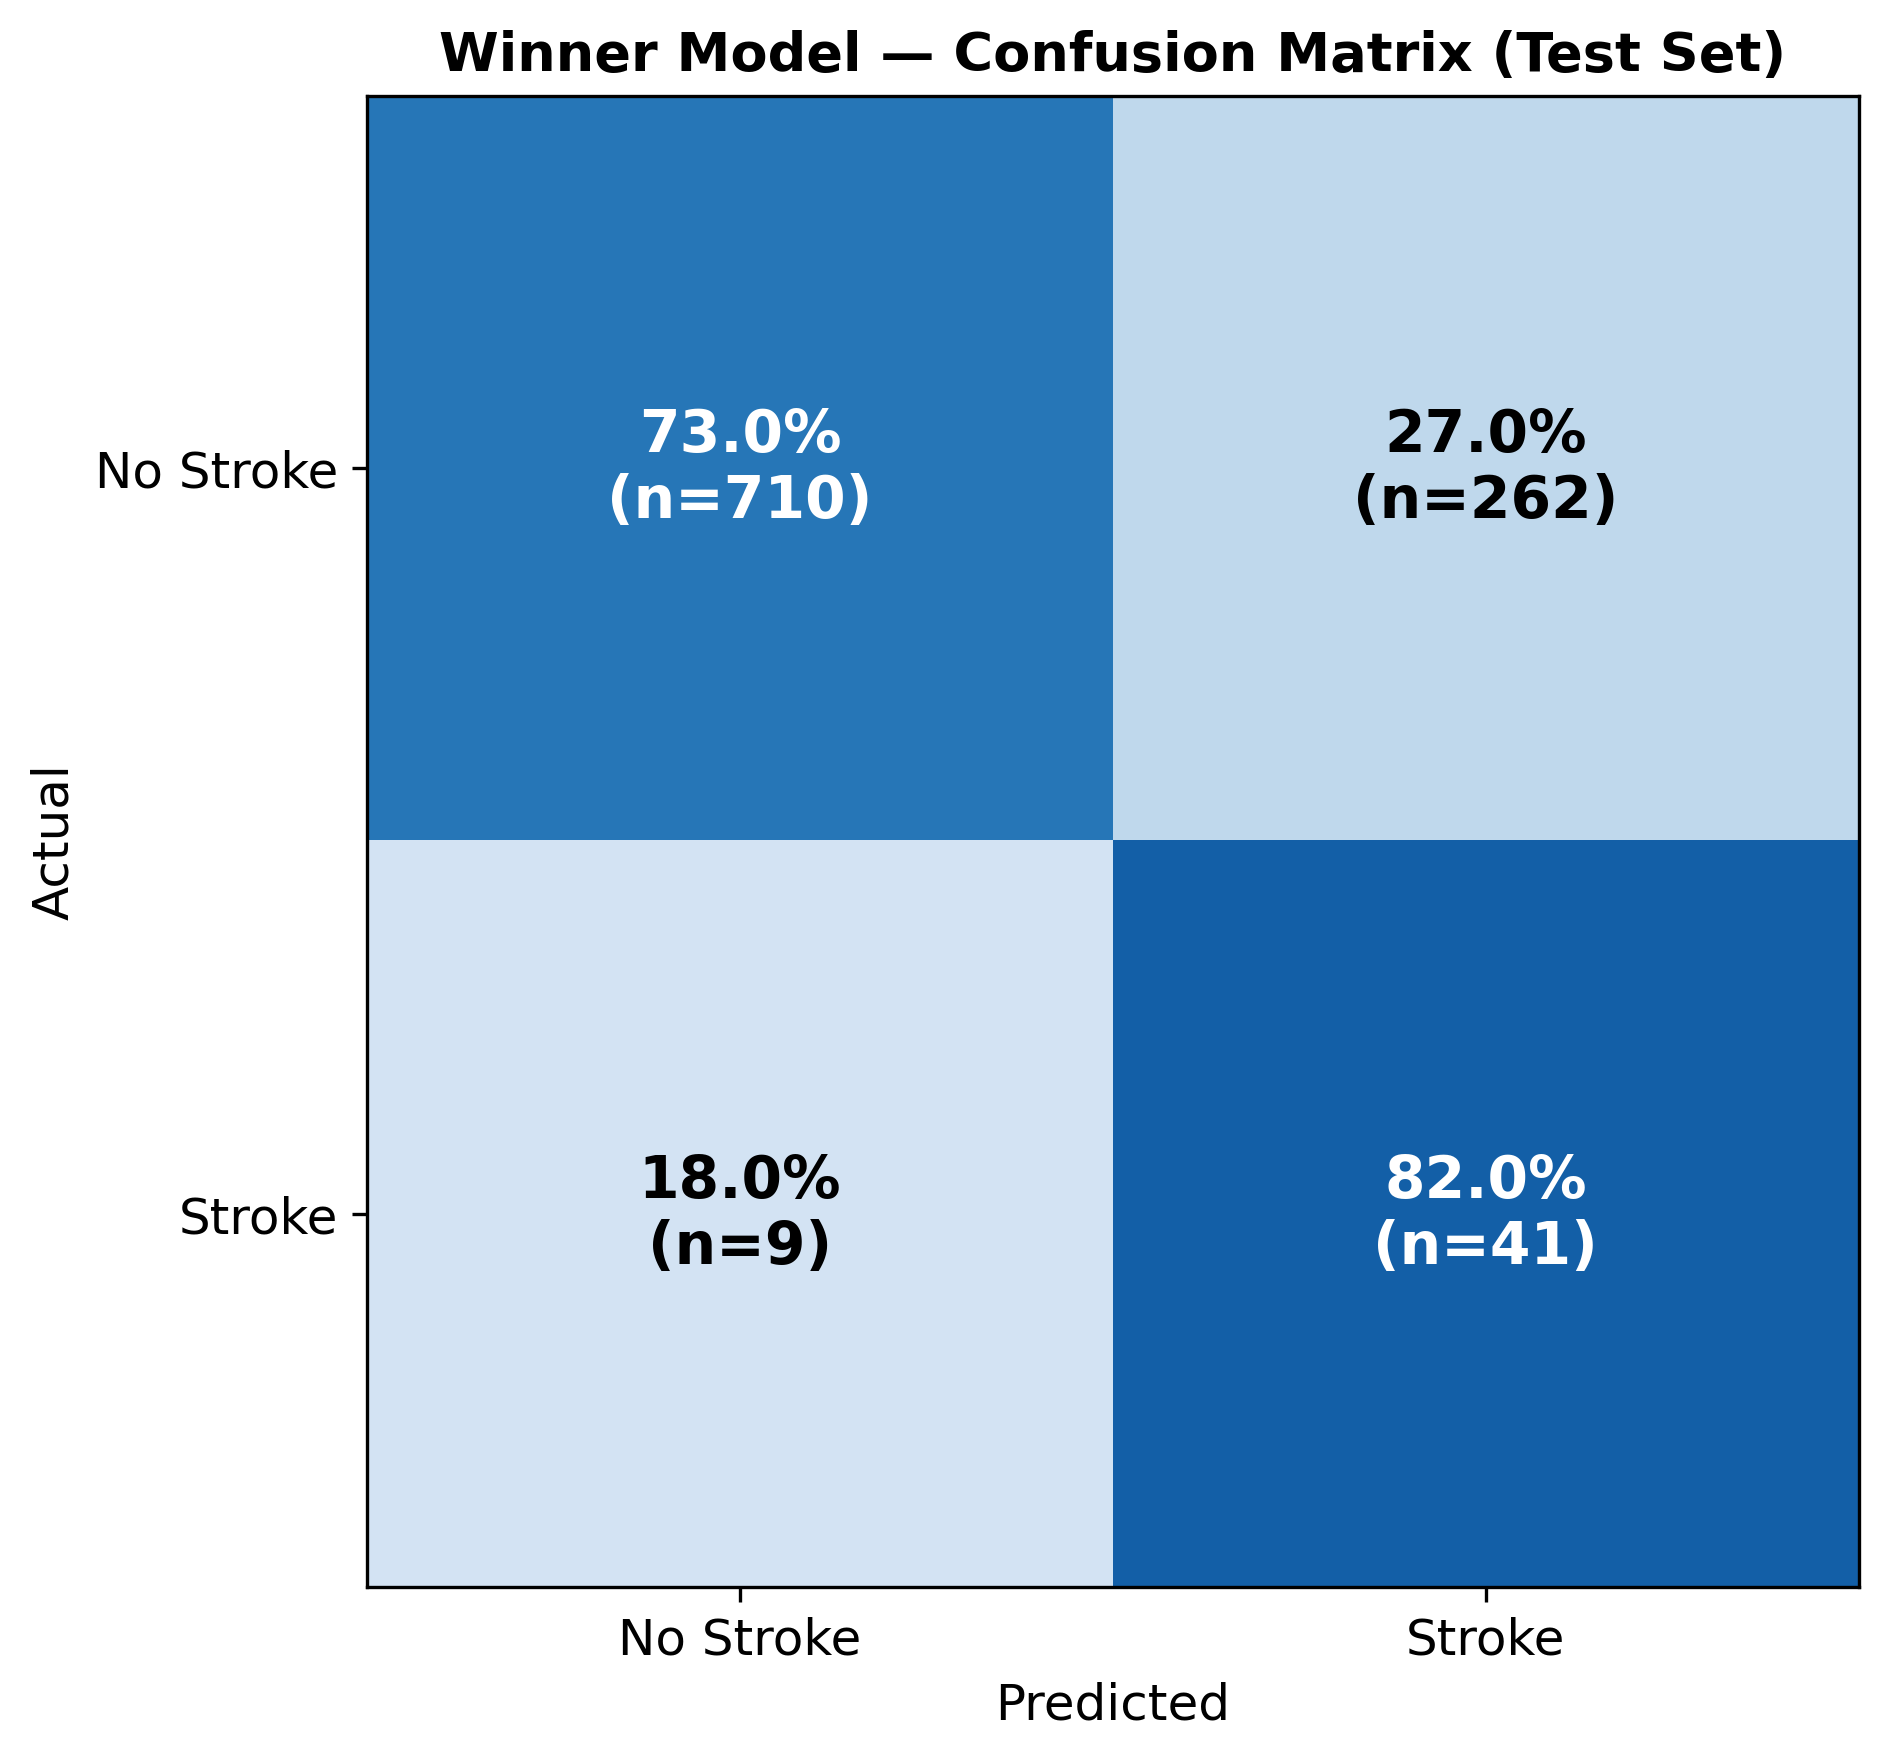
\includegraphics[width=\linewidth]{winner_analysis/confusion_matrix.png}
    \caption{Confusion matrix.}
    \label{fig:cm}
  \end{subfigure}
  \caption{Winner model evaluation plots.}
\end{figure}

\subsubsection{Threshold Analysis}

Figure~\ref{fig:threshold} shows how precision, recall, and F1 change as a function of the decision threshold.
The default threshold of $0.5$ is far from optimal for imbalanced data.

\begin{figure}[H]
  \centering
  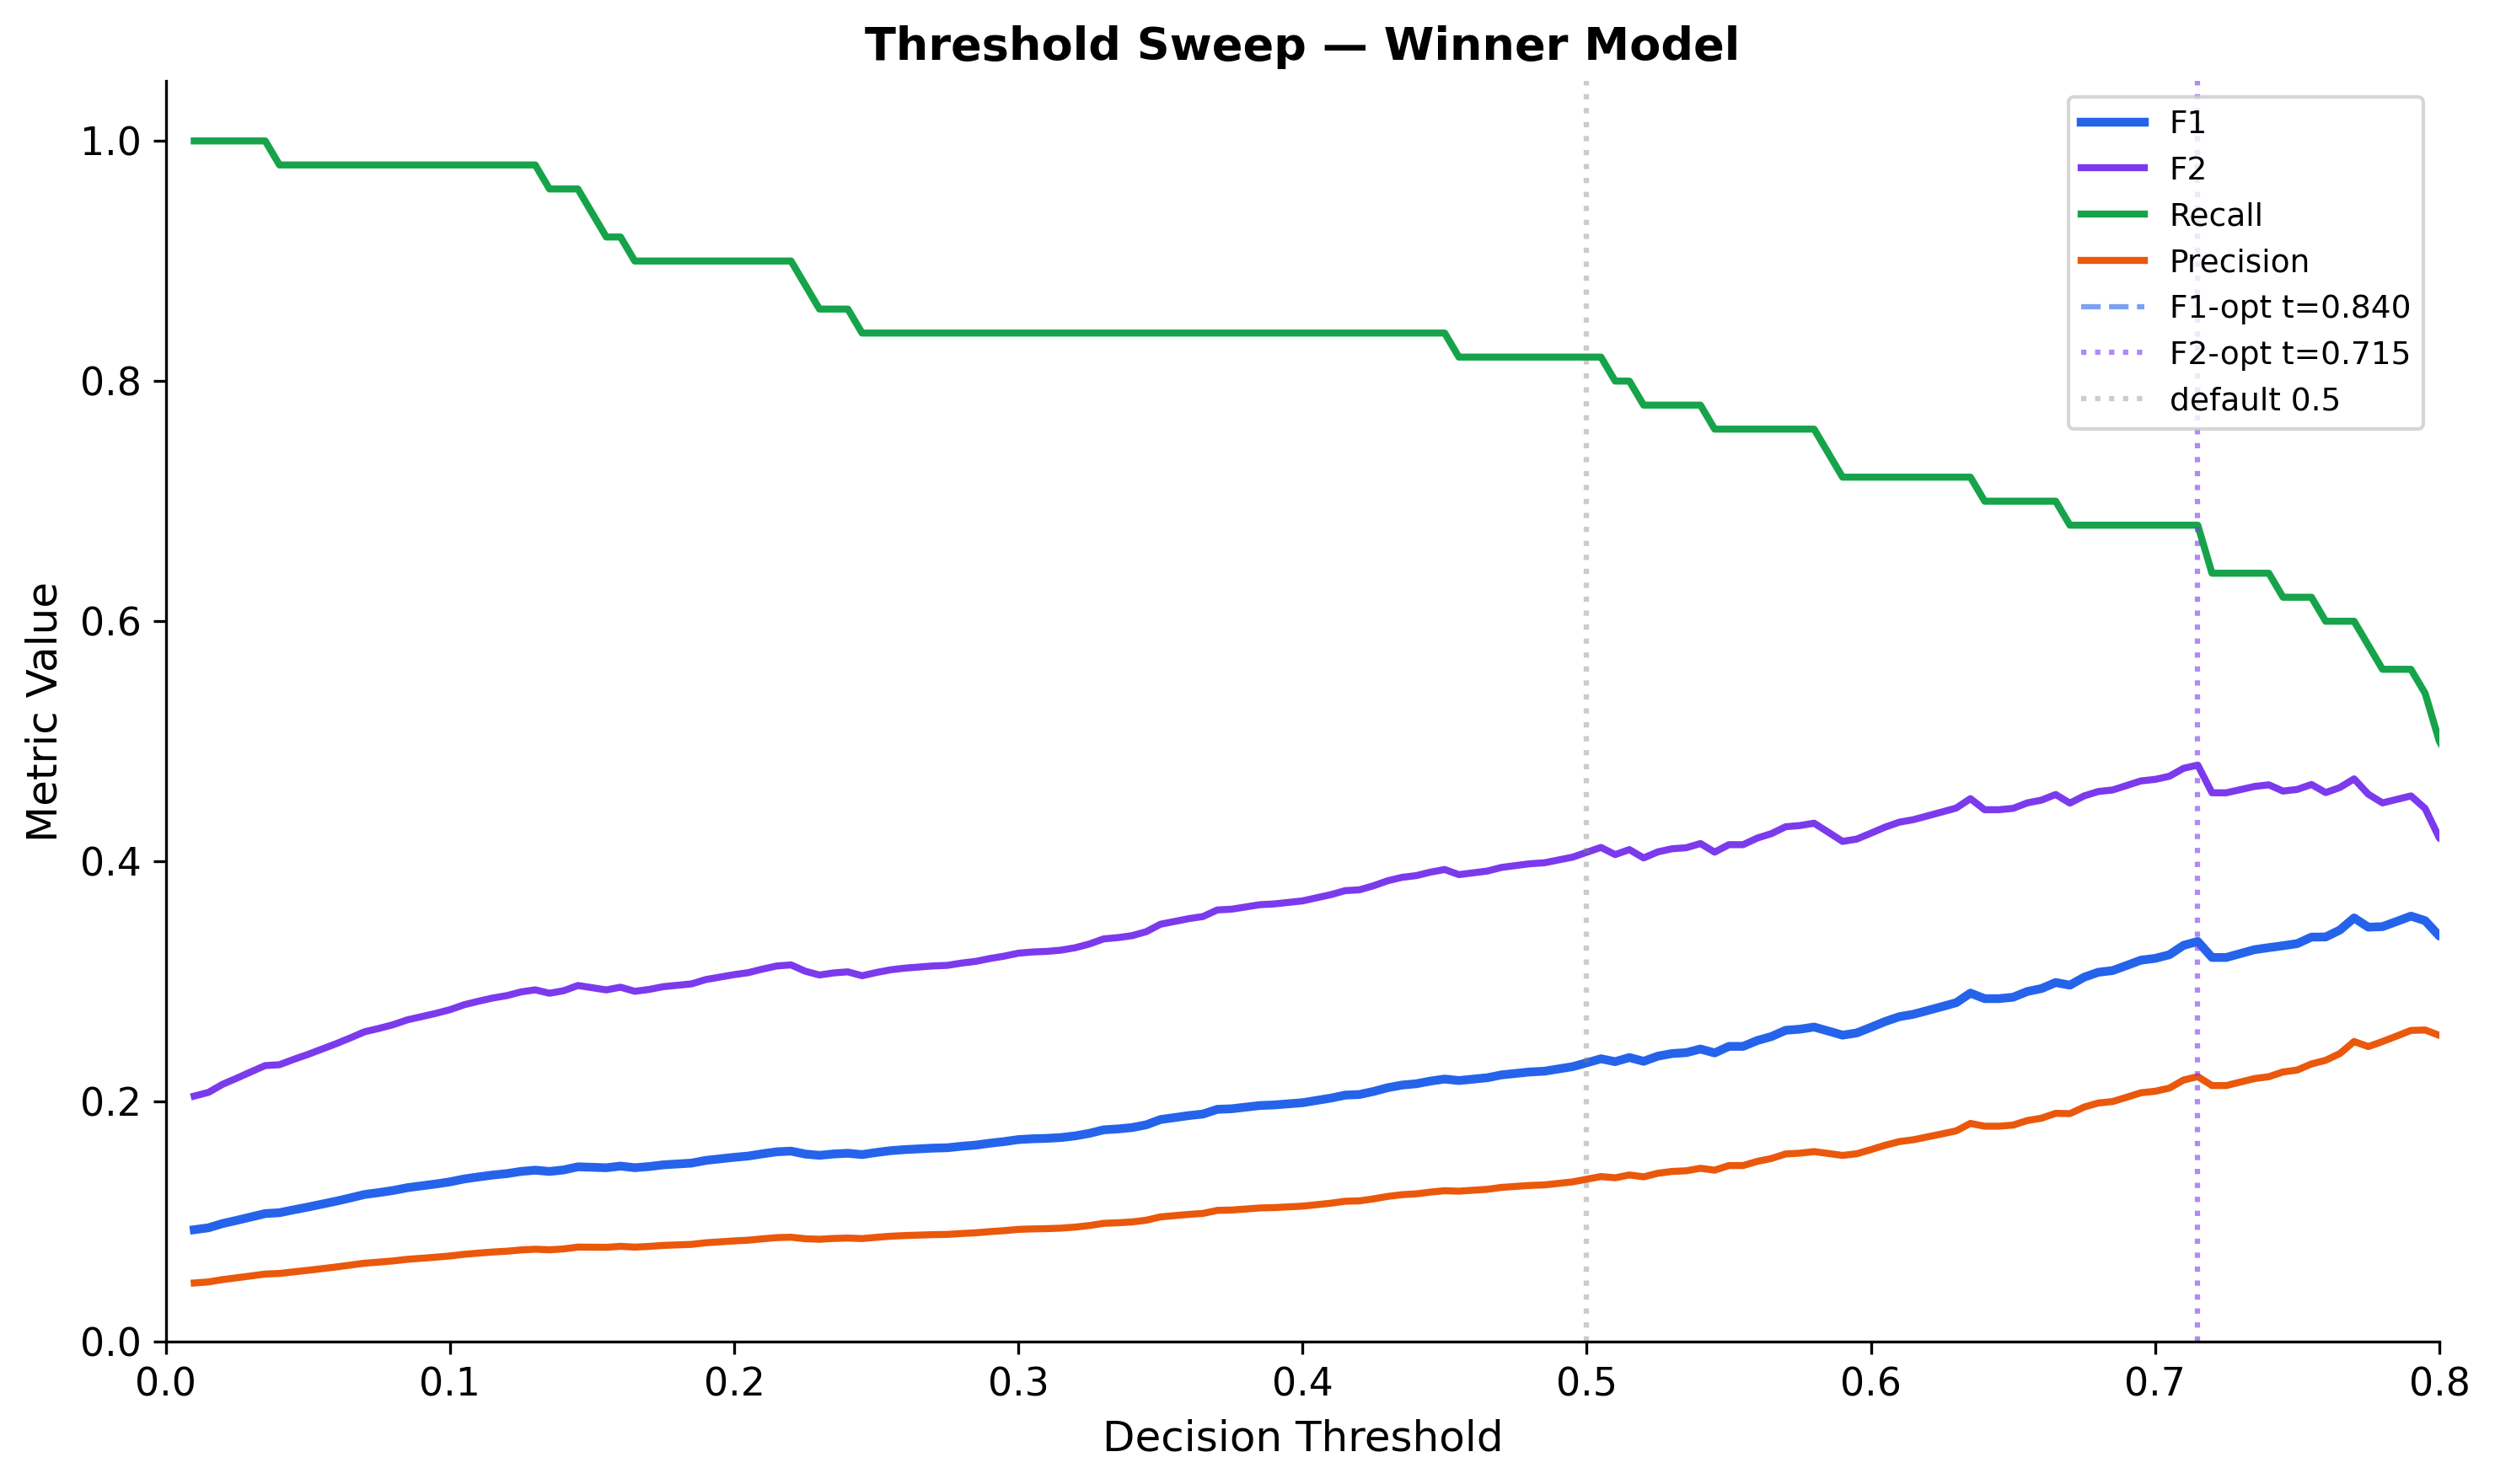
\includegraphics[width=0.7\linewidth]{winner_analysis/threshold_sweep.png}
  \caption{Threshold sweep: Precision, Recall, and F1 as a function of decision threshold $t$. The F1-optimal threshold $t^*=0.84$ yields F1$=0.372$, Recall$=42\%$, Precision$=33.3\%$.}
  \label{fig:threshold}
\end{figure}

Three clinically meaningful operating points are summarised in Table~\ref{tab:thresholds}.

\begin{table}[H]
  \centering
  \caption{Operating points for the winner model at different decision thresholds.}
  \label{tab:thresholds}
  \begin{tabular}{lccccc}
    \toprule
    \textbf{Mode} & \textbf{Threshold} & \textbf{Recall} & \textbf{Precision} & \textbf{F1} \\
    \midrule
    Screening (high recall)   & 0.135 & 90.00\% &  8.21\% & 0.150 \\
    Balanced ($t^*$)           & 0.840 & 42.00\% & 33.33\% & 0.372 \\
    Confirmatory (high prec.) & 0.875 & 30.00\% & 30.61\% & 0.303 \\
    \bottomrule
  \end{tabular}
\end{table}

\subsection{Calibration}

Figure~\ref{fig:calibration} compares reliability diagrams before and after calibration.

\begin{figure}[H]
  \centering
  \begin{subfigure}[b]{0.48\linewidth}
    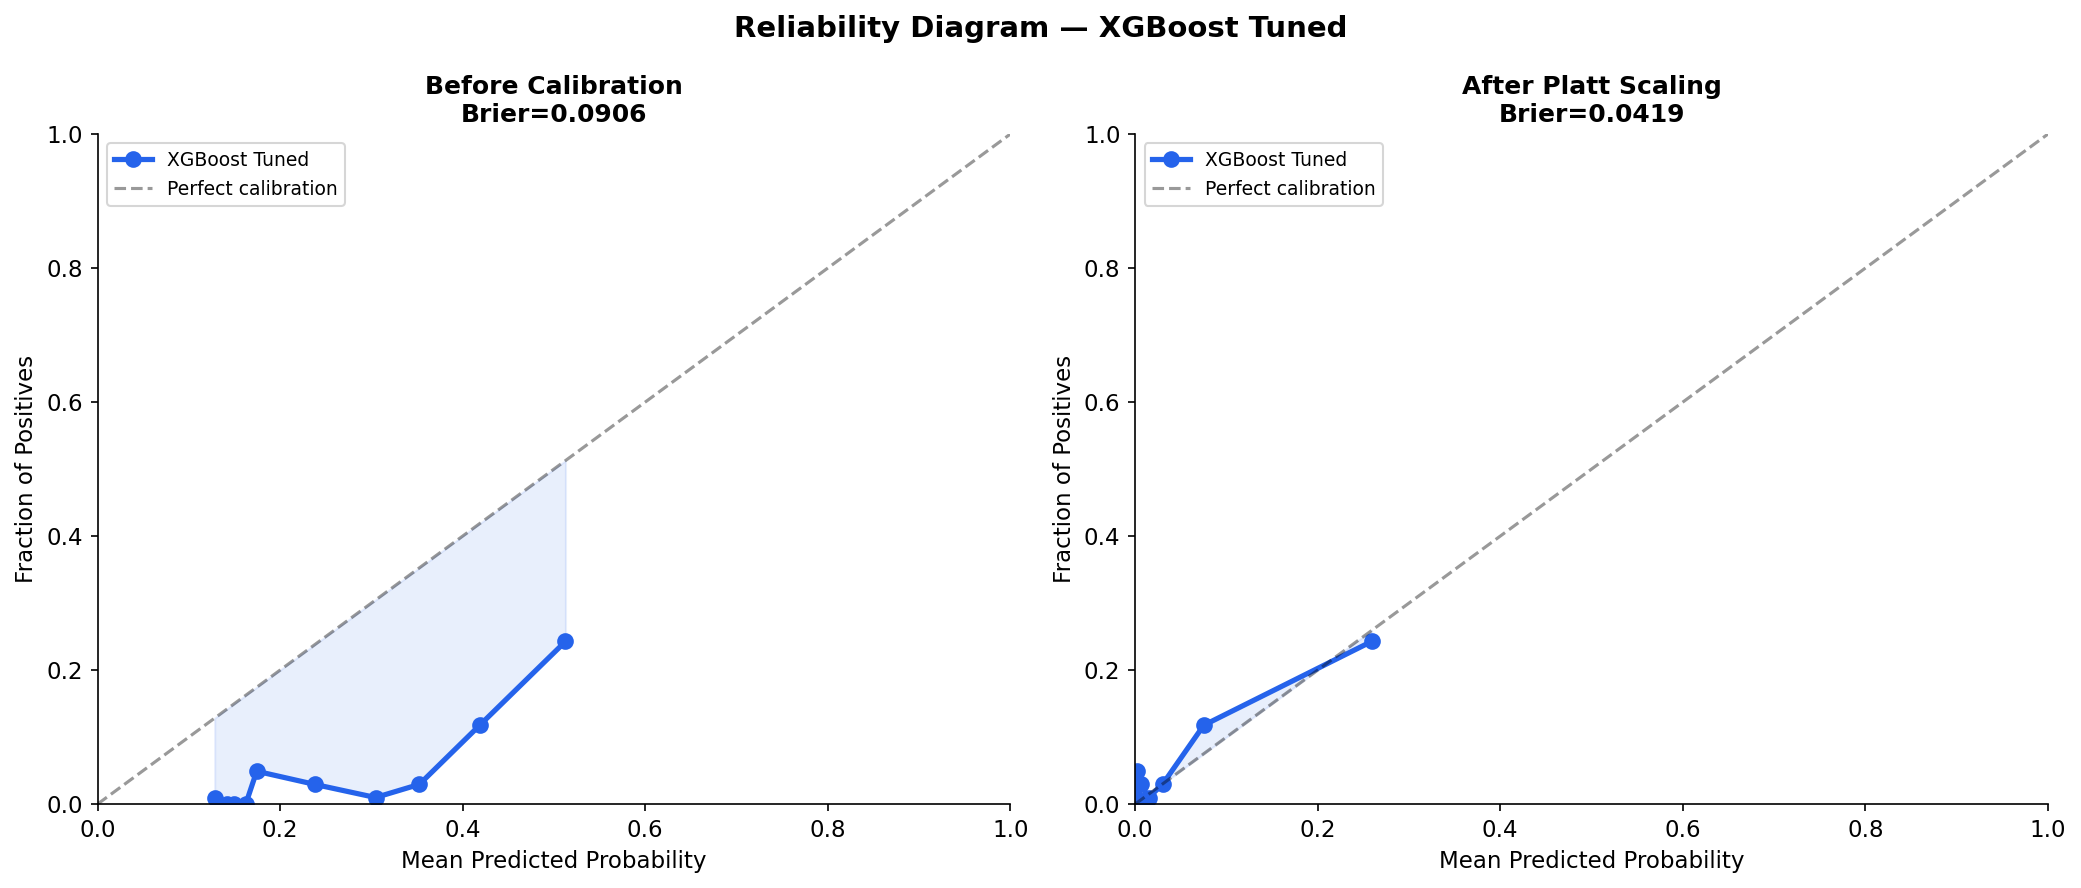
\includegraphics[width=\linewidth]{winner_analysis/calibration_curve.png}
    \caption{Winner model calibration curve.}
  \end{subfigure}
  \hfill
  \begin{subfigure}[b]{0.48\linewidth}
    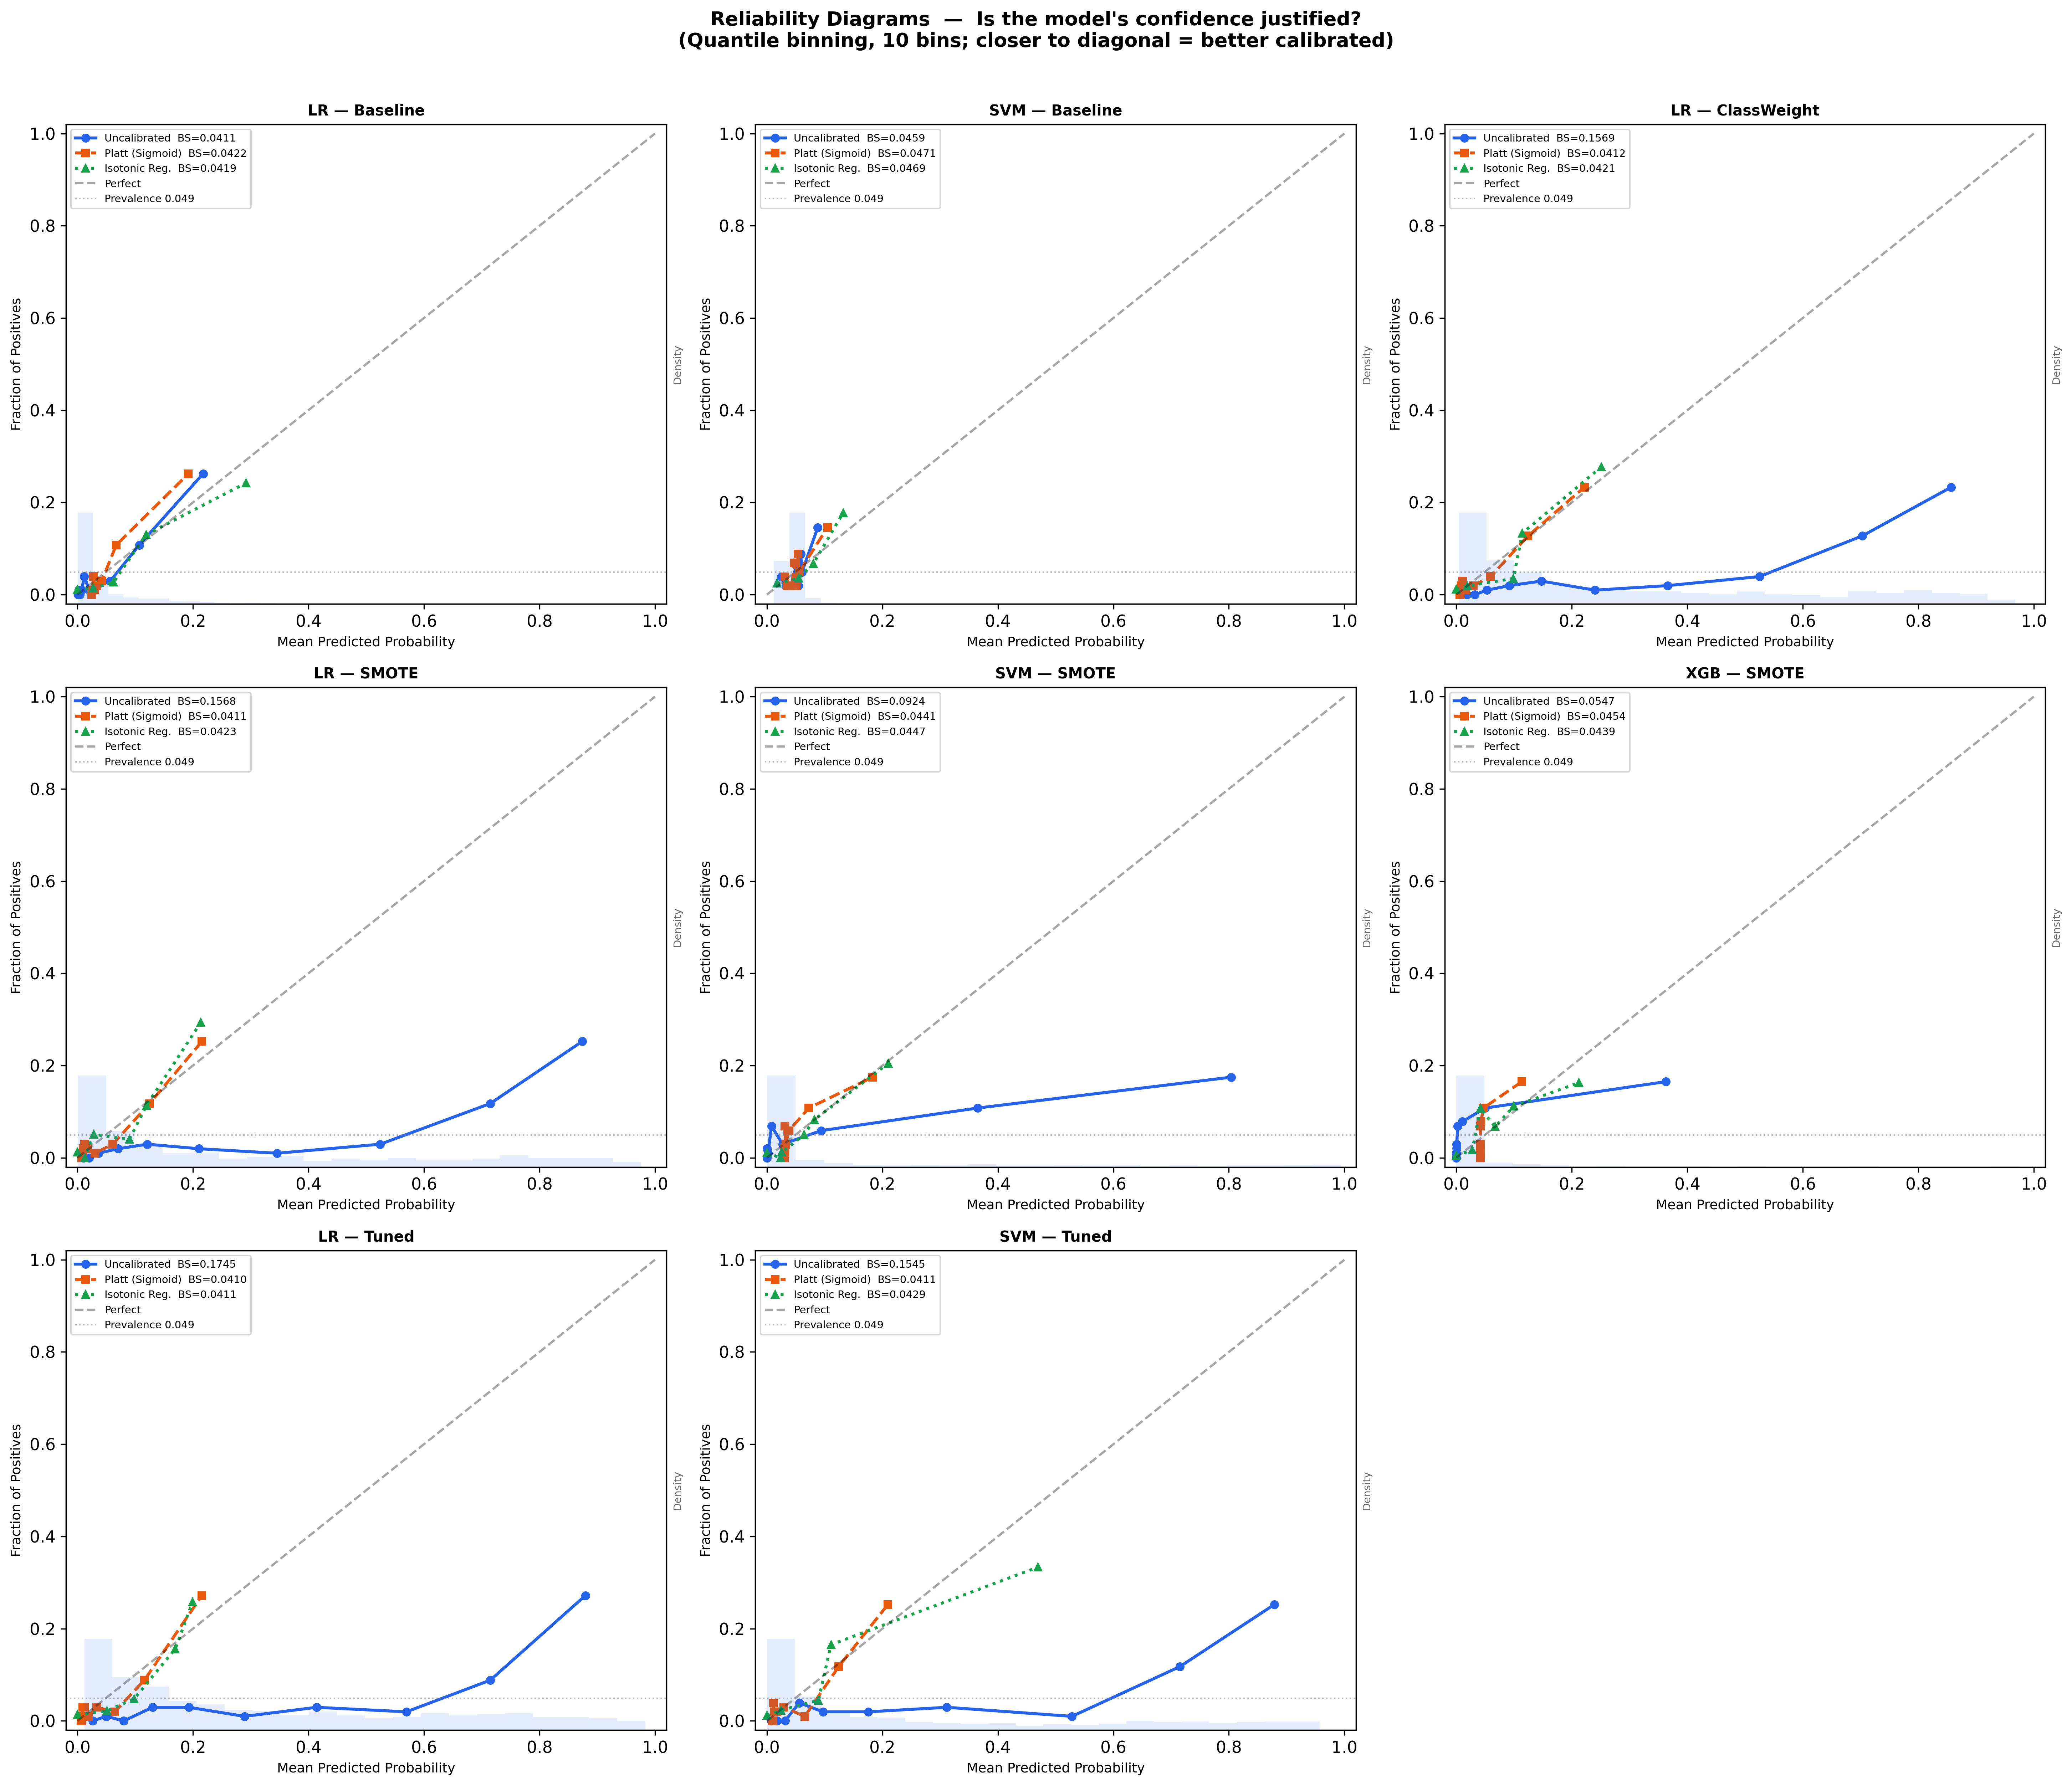
\includegraphics[width=\linewidth]{reliability_diagrams.png}
    \caption{Reliability diagrams across all models.}
  \end{subfigure}
  \caption{Calibration plots. A perfectly calibrated model would follow the diagonal.}
  \label{fig:calibration}
\end{figure}

\begin{table}[H]
  \centering
  \caption{Brier scores before and after post-hoc calibration (winner model).}
  \label{tab:brier}
  \begin{tabular}{lcc}
    \toprule
    \textbf{Configuration} & \textbf{Brier Score} & \textbf{Reduction} \\
    \midrule
    Uncalibrated            & 0.1689 & — \\
    Platt Scaling           & 0.0410 & $\downarrow\,75.7\%$ \\
    Isotonic Regression     & 0.0411 & $\downarrow\,75.6\%$ \\
    \bottomrule
  \end{tabular}
\end{table}

Calibration dramatically improves probability reliability without altering the decision boundary.
Both Platt scaling and isotonic regression achieve similar reductions; Platt scaling is preferred for its lower overfitting risk on small datasets.

\subsection{Feature Importance and Interpretability}

\begin{figure}[H]
  \centering
  \begin{subfigure}[b]{0.48\linewidth}
    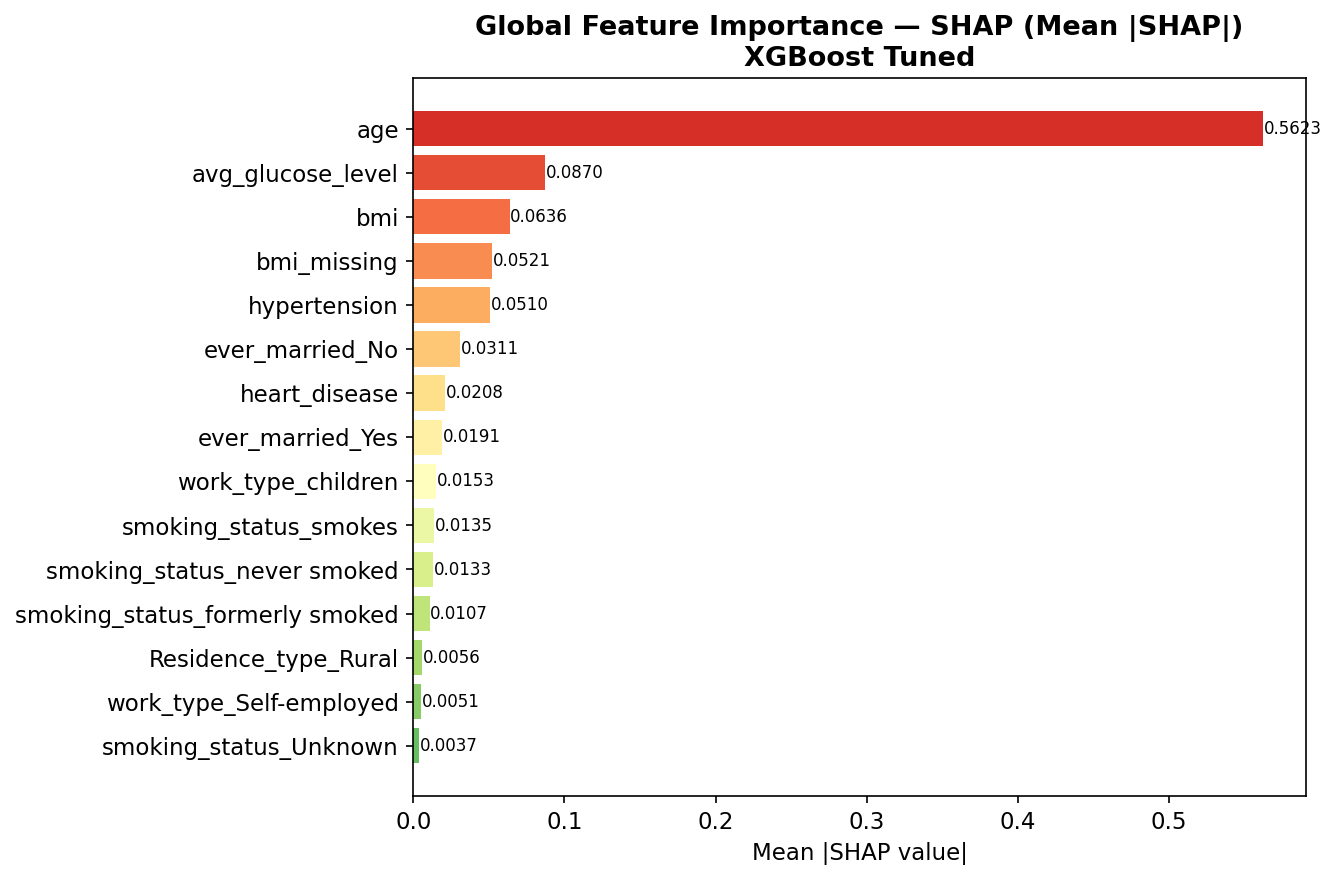
\includegraphics[width=\linewidth]{shap_lime/shap_bar.png}
    \caption{SHAP: mean absolute feature importance.}
  \end{subfigure}
  \hfill
  \begin{subfigure}[b]{0.48\linewidth}
    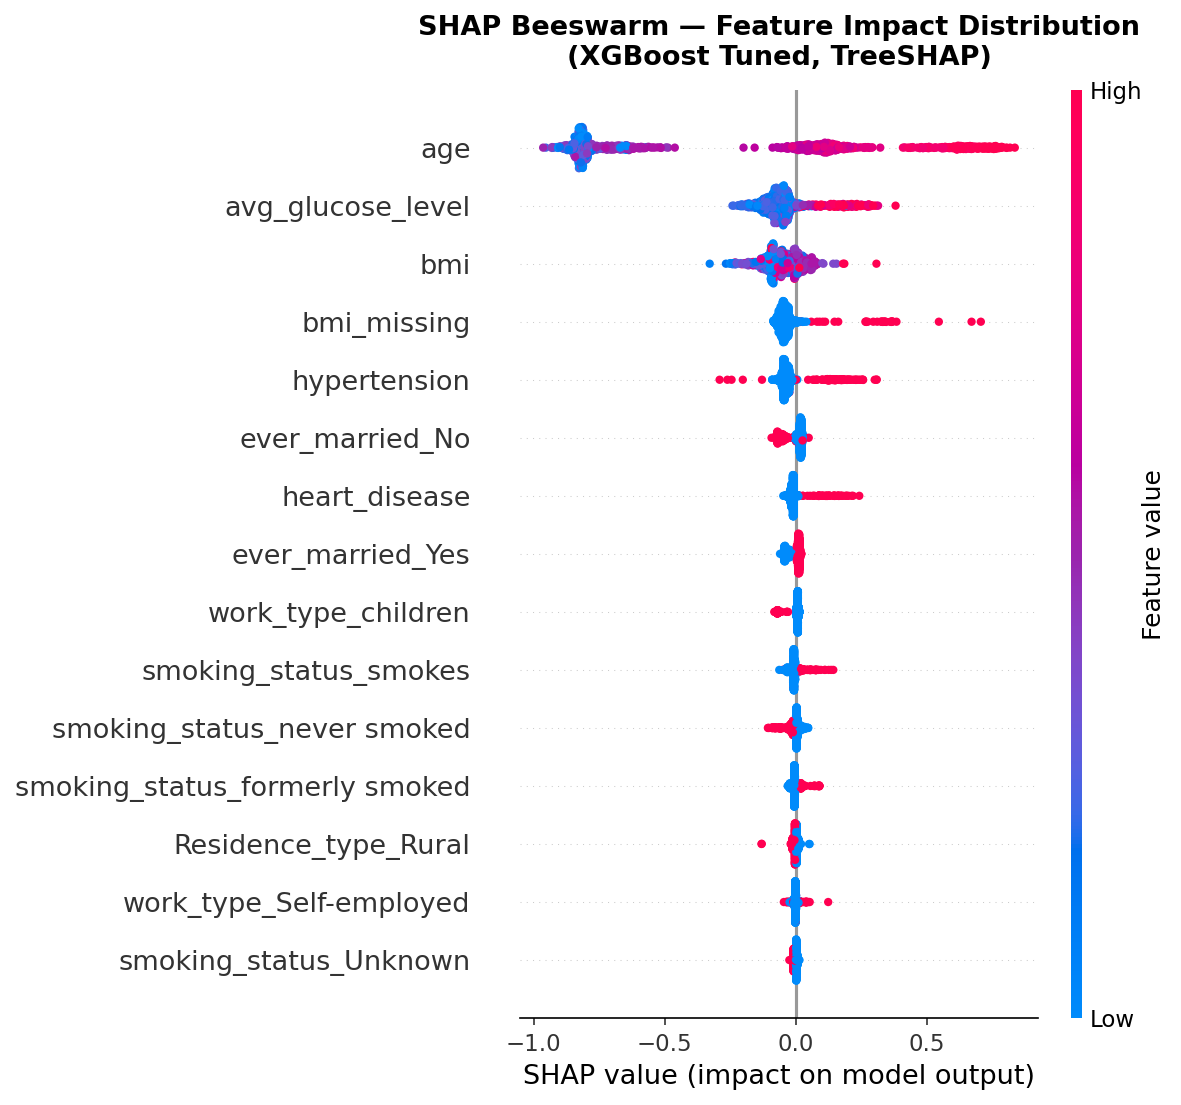
\includegraphics[width=\linewidth]{shap_lime/shap_beeswarm.png}
    \caption{SHAP: beeswarm (direction of effects).}
  \end{subfigure}
  \caption{Global SHAP explanations for the winner model.}
  \label{fig:shap}
\end{figure}

\begin{table}[H]
  \centering
  \caption{Top-10 features by mean $|\text{SHAP}|$ value.}
  \label{tab:shap}
  \begin{tabular}{clc}
    \toprule
    \textbf{Rank} & \textbf{Feature} & \textbf{Mean $|\text{SHAP}|$} \\
    \midrule
    1  & \texttt{age}                     & 0.5623 \\
    2  & \texttt{avg\_glucose\_level}     & 0.0870 \\
    3  & \texttt{bmi}                     & 0.0636 \\
    4  & \texttt{bmi\_missing}            & 0.0521 \\
    5  & \texttt{hypertension}            & 0.0510 \\
    6  & \texttt{ever\_married\_No}       & 0.0311 \\
    7  & \texttt{heart\_disease}          & 0.0208 \\
    8  & \texttt{ever\_married\_Yes}      & 0.0191 \\
    9  & \texttt{work\_type\_children}    & 0.0153 \\
    10 & \texttt{smoking\_status\_smokes} & 0.0135 \\
    \bottomrule
  \end{tabular}
\end{table}

\textbf{Discussion.}
Age dominates all other features by a large margin (SHAP $=0.562$, roughly $6\times$ the next feature), consistent with the statistical tests and clinical literature.
Glucose level and BMI are second and third.
Hypertension and heart disease have similar SHAP values, consistent with their similar odds ratios in Table~\ref{tab:stat_tests}.
The engineered \texttt{bmi\_missing} indicator (rank 4) is more informative than hypertension, validating the decision to add it.

Figure~\ref{fig:lime} shows local LIME explanations for representative cases.

\begin{figure}[H]
  \centering
  \begin{subfigure}[b]{0.48\linewidth}
    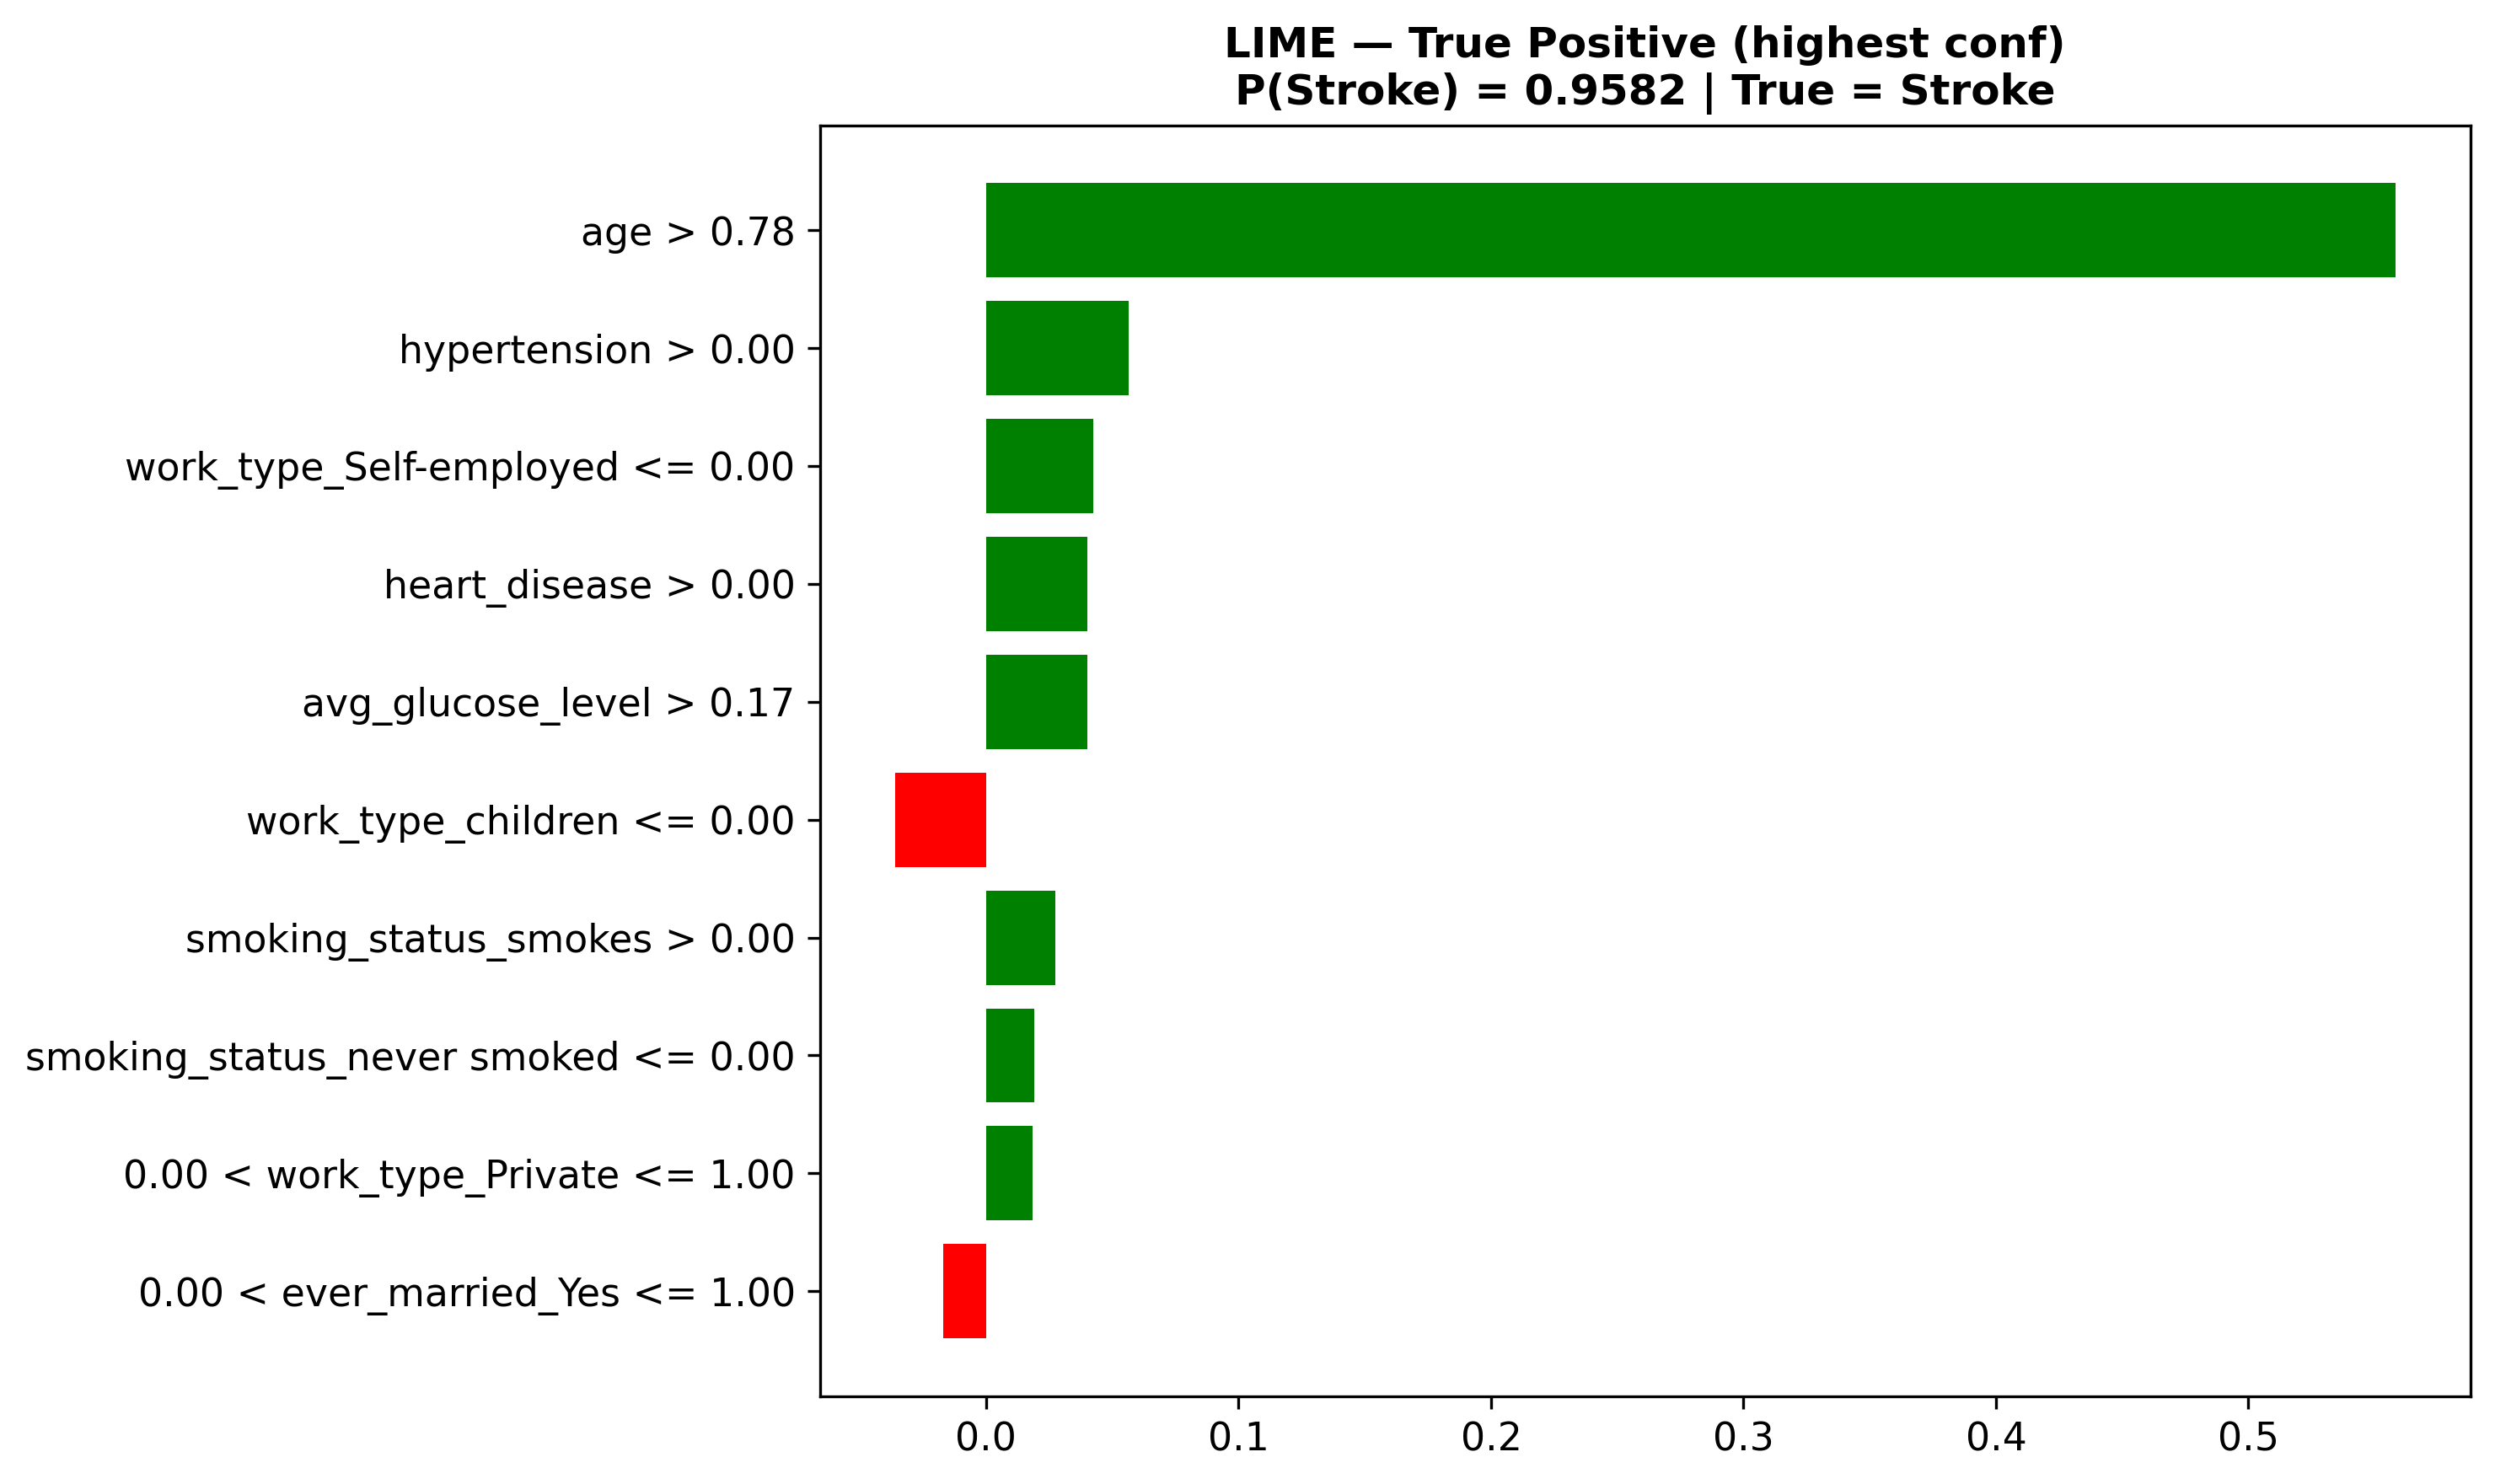
\includegraphics[width=\linewidth]{winner_analysis/lime_true_positive_highest_conf.png}
    \caption{True Positive (high-confidence stroke).}
  \end{subfigure}
  \hfill
  \begin{subfigure}[b]{0.48\linewidth}
    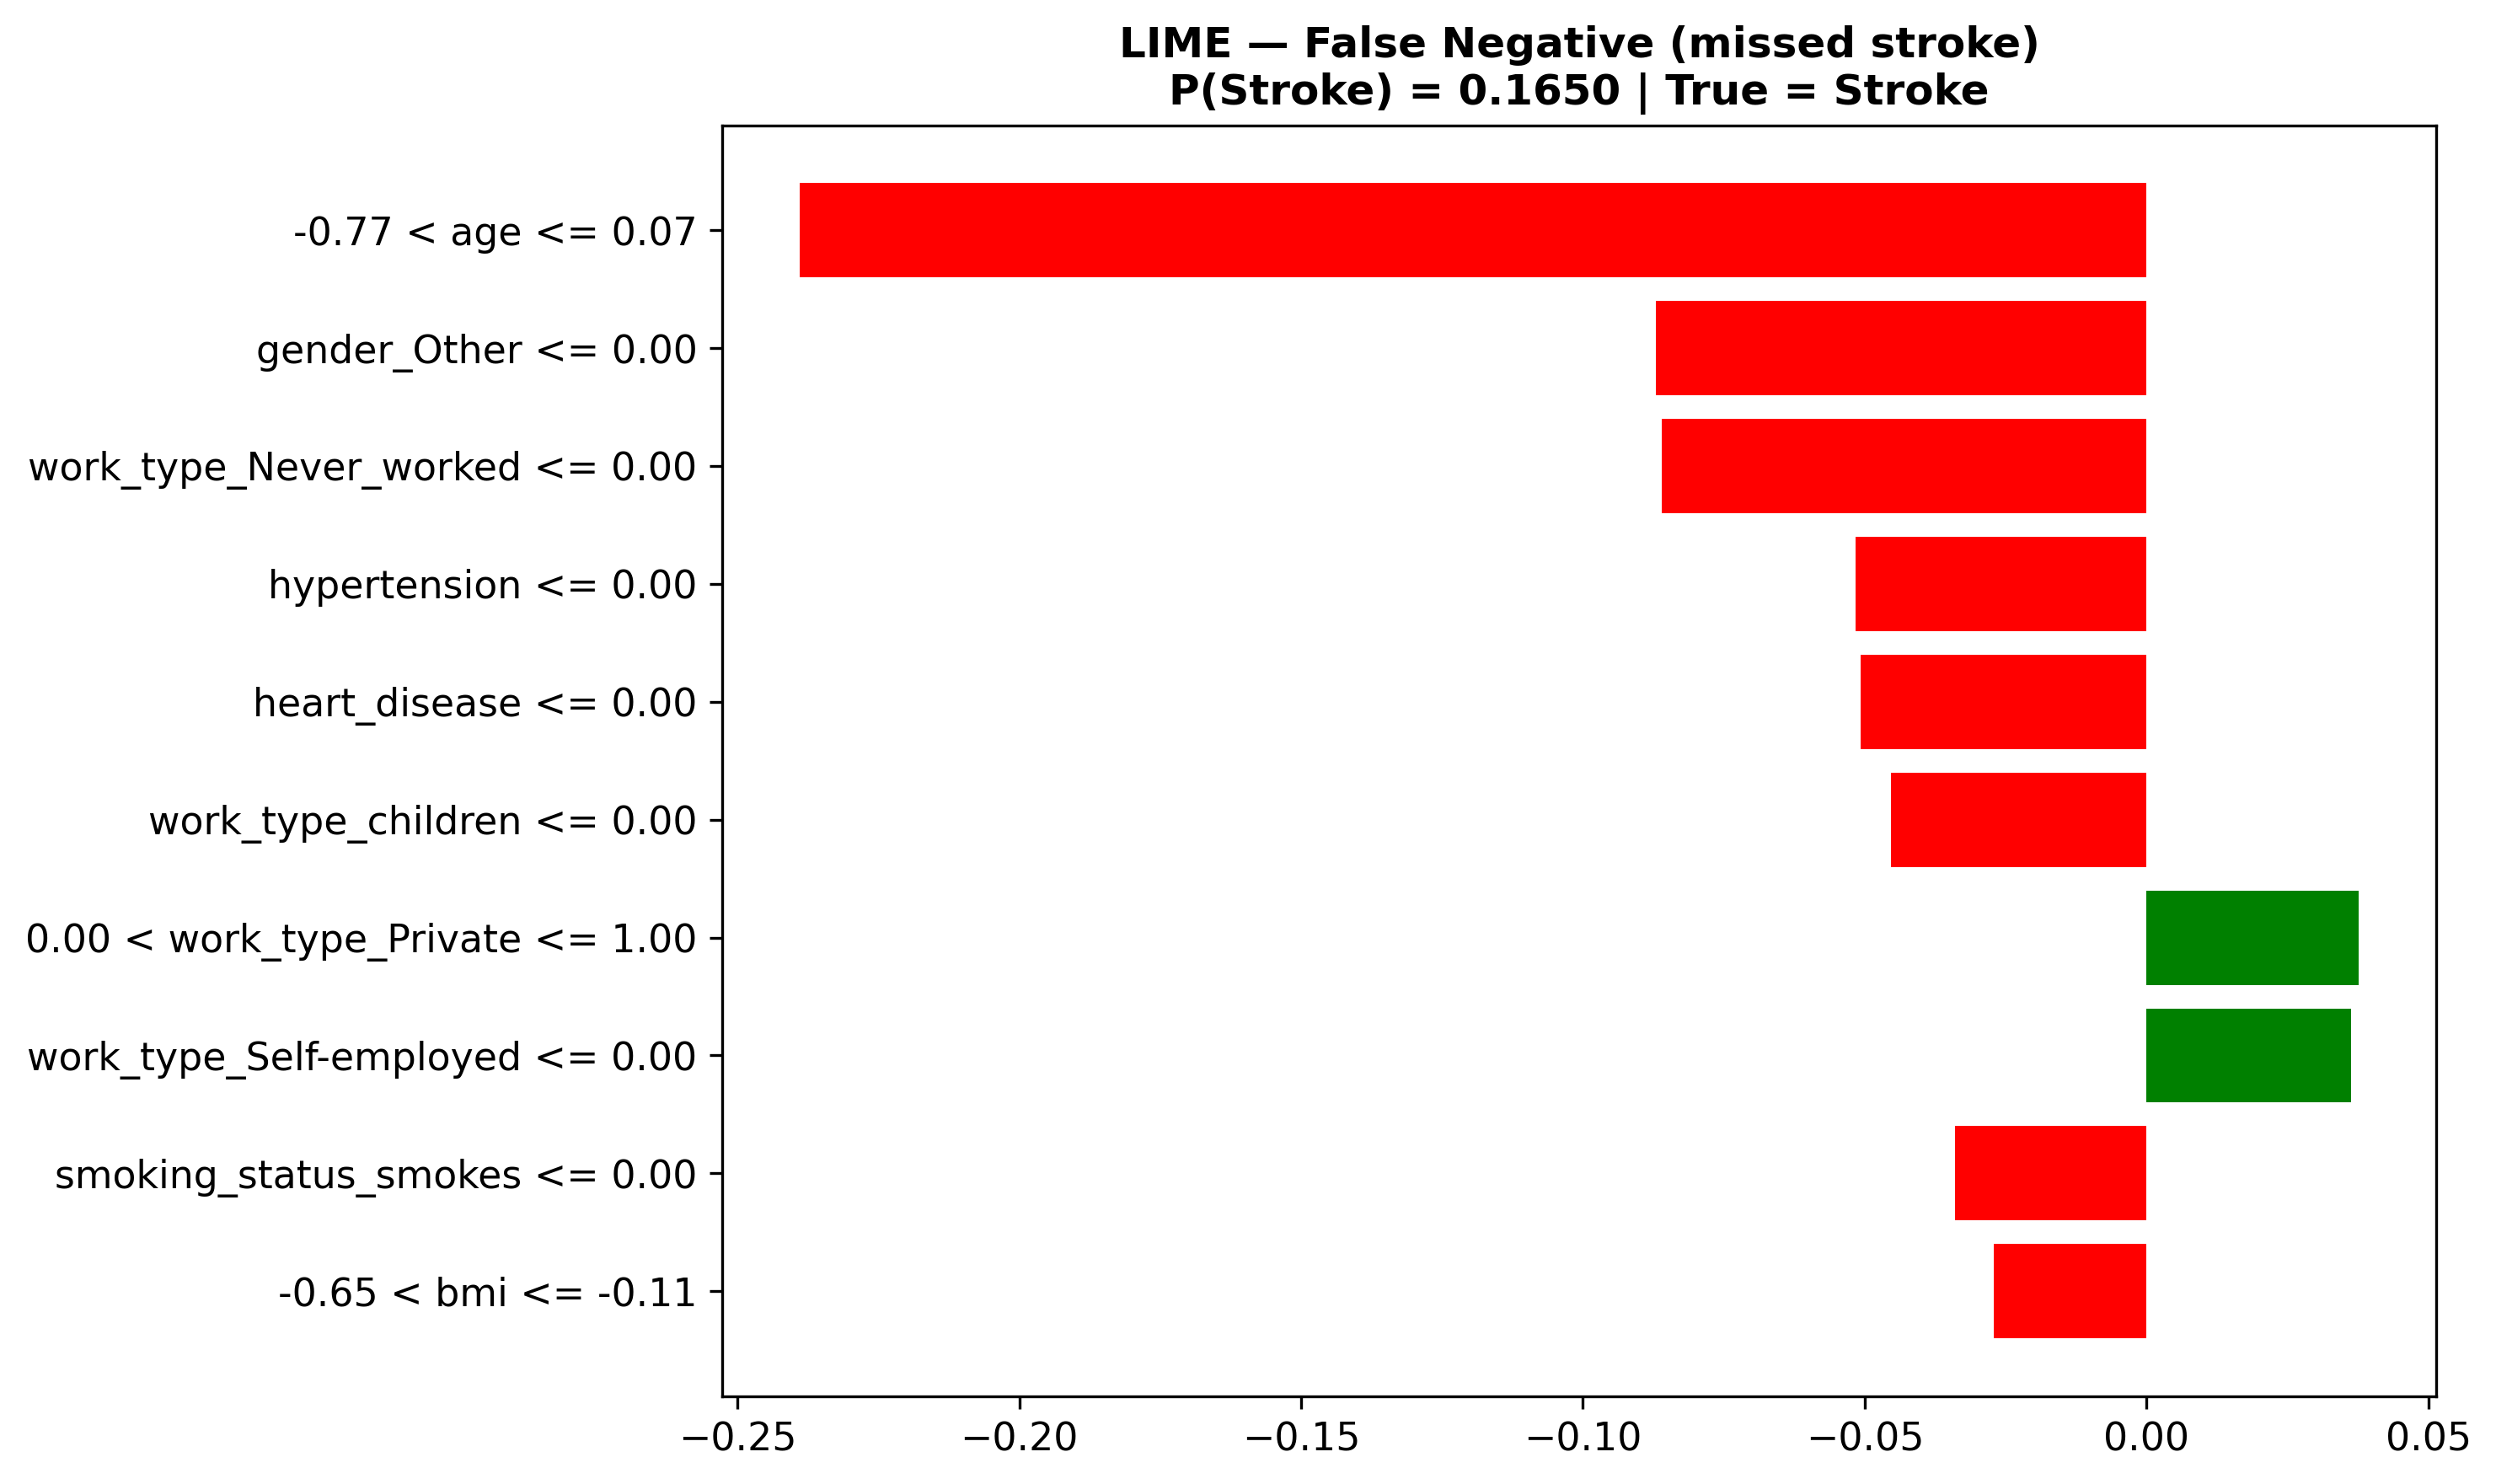
\includegraphics[width=\linewidth]{winner_analysis/lime_false_negative_missed_stroke.png}
    \caption{False Negative (missed stroke case).}
  \end{subfigure}
  \caption{LIME local explanations for representative test cases.}
  \label{fig:lime}
\end{figure}

\subsection{Comprehensive Model Comparison}

Figure~\ref{fig:master} provides a summary comparison across all evaluated configurations.

\begin{figure}[H]
  \centering
  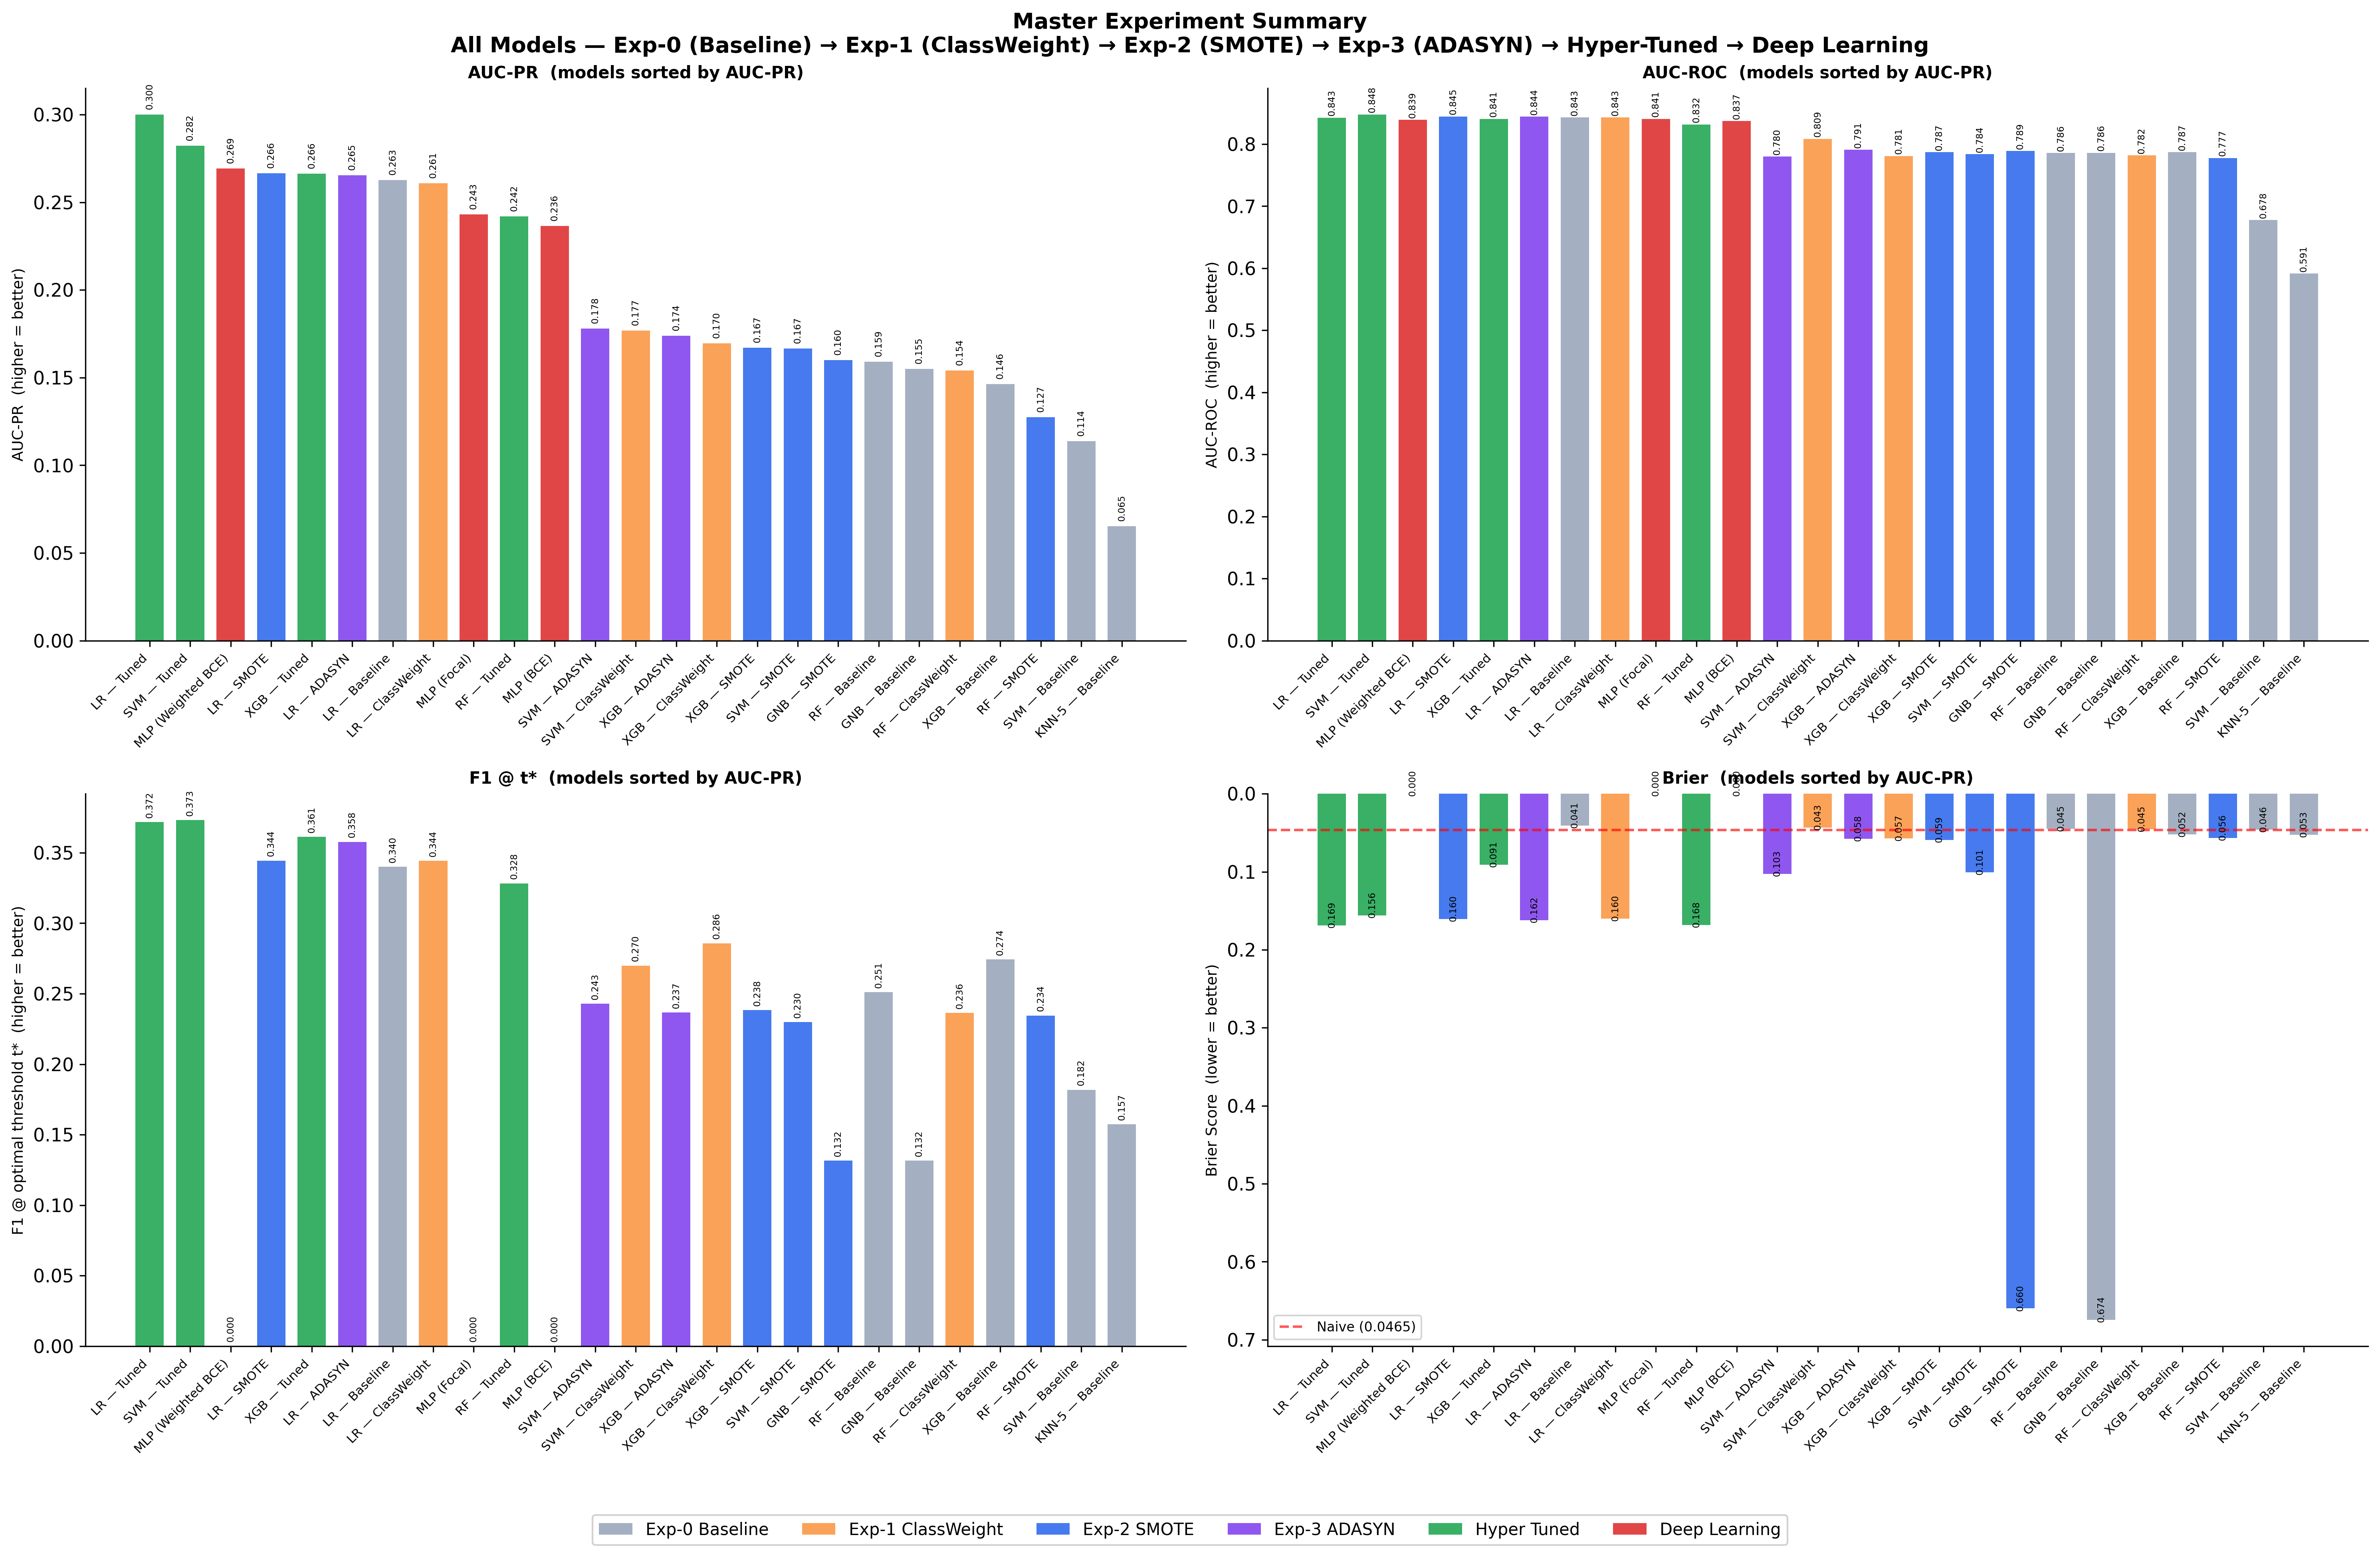
\includegraphics[width=0.92\linewidth]{master_summary_figure.png}
  \caption{Master summary figure: AUC-PR, Recall, Precision, and F1 across all models and imbalance strategies.}
  \label{fig:master}
\end{figure}

% ============================================================
\section{Conclusions}
\label{sec:conclusions}
% ============================================================

\subsection{Key Findings}

\begin{enumerate}
  \item \textbf{Accuracy is not a valid metric for imbalanced medical data.}
        Baseline models achieve $>95\%$ accuracy while detecting fewer than $4\%$ of actual stroke cases.
        AUC-PR is the appropriate primary metric for this problem.

  \item \textbf{Class weighting is the most effective single intervention.}
        It raises LR recall from $2\%$ to $80\%$ while preserving AUC-PR.
        SMOTE and ADASYN provide similar gains; ADASYN offers no clear advantage for this dataset.

  \item \textbf{Threshold tuning is complementary and highly effective.}
        Post-hoc threshold optimisation raises F1 from $0.245$ to $0.372$ for LR at the balanced operating point—a larger gain than any resampling strategy alone.

  \item \textbf{A simple linear model wins.}
        The hyperparameter-tuned Logistic Regression achieves the highest AUC-PR ($0.300$) of all configurations, outperforming XGBoost ($0.266$) and the MLP ($0.269$) on the primary metric.
        For tabular clinical data at this scale, interpretability and cost-sensitivity matter more than model complexity.

  \item \textbf{Calibration is essential for deployment.}
        Post-hoc Platt scaling reduces the Brier score by $75.7\%$ (from $0.169$ to $0.041$), enabling reliable probability-based triage decisions.

  \item \textbf{Age is the dominant clinical predictor.}
        SHAP analysis confirms age as overwhelmingly the most important feature ($6\times$ the next feature), consistent with established clinical risk factors for stroke.
\end{enumerate}

\subsection{Methods Learned}

This project provided hands-on experience with: the precision-recall trade-off in imbalanced learning; the difference between ranking metrics (AUC-ROC/PR) and calibration metrics (Brier score); the mechanics of SMOTE, ADASYN, and cost-sensitive learning; threshold engineering for different clinical deployment scenarios; and model-agnostic explanation tools (SHAP, LIME, permutation importance).

\subsection{Future Directions}

\begin{itemize}
  \item \textbf{Richer features:} Incorporating blood pressure readings, cholesterol levels, and imaging biomarkers could substantially improve predictive power.
  \item \textbf{Hospital-grade validation:} Prospective validation on an independent clinical cohort, accounting for temporal drift and hospital-specific distributions.
  \item \textbf{Fairness audit:} Examining whether the model's performance is equitable across demographic subgroups (age bands, gender).
  \item \textbf{Temporal modelling:} Using longitudinal patient records with recurrent architectures to capture risk trajectory over time.
\end{itemize}

% ============================================================
\section{Workload Distribution}
\label{sec:workload}
% ============================================================

\begin{table}[H]
  \centering
  \caption{Team member contributions.}
  \label{tab:workload}
  \renewcommand{\arraystretch}{1.15}
  \begin{tabular}{lp{10cm}}
    \toprule
    \textbf{Member} & \textbf{Contributions} \\
    \midrule
    Nevzat Han Alt\i{}n &
      Exploratory data analysis (\texttt{01\_eda.py}); statistical significance testing; EDA figures; data sanity checks (\texttt{00\_sanity\_checks.py}). \\
    \addlinespace
    Ahmet B\"uy\"ukberber &
      Classical ML baseline (\texttt{02\_classical\_ml.py}); Experiment 0 (baseline) and Experiment 1 (class weighting); baseline result visualisations. \\
    \addlinespace
    Veli Karakaya &
      Experiments 2–3 (SMOTE, ADASYN); hyperparameter search pipeline (\texttt{03\_hyper/run\_search.py}); winner model analysis; report writing. \\
    \addlinespace
    Ece \c{S}e\c{s}en &
      PyTorch MLP implementation (\texttt{08\_dl\_mlp/}); focal loss; deep learning experiments; DL comparison analysis. \\
    \addlinespace
    Umut \c{C}a\u{g}\i{}n \"Ozcan &
      Threshold tuning (\texttt{07\_exp4\_threshold.py}); calibration analysis (\texttt{09\_calibration\_summary.py}); SHAP/LIME interpretability (\texttt{11\_shap\_lime\_global.py}); presentation. \\
    \bottomrule
  \end{tabular}
\end{table}

% ============================================================
\appendix
\section{Additional Figures}
\label{app:figures}
% ============================================================

\begin{figure}[H]
  \centering
  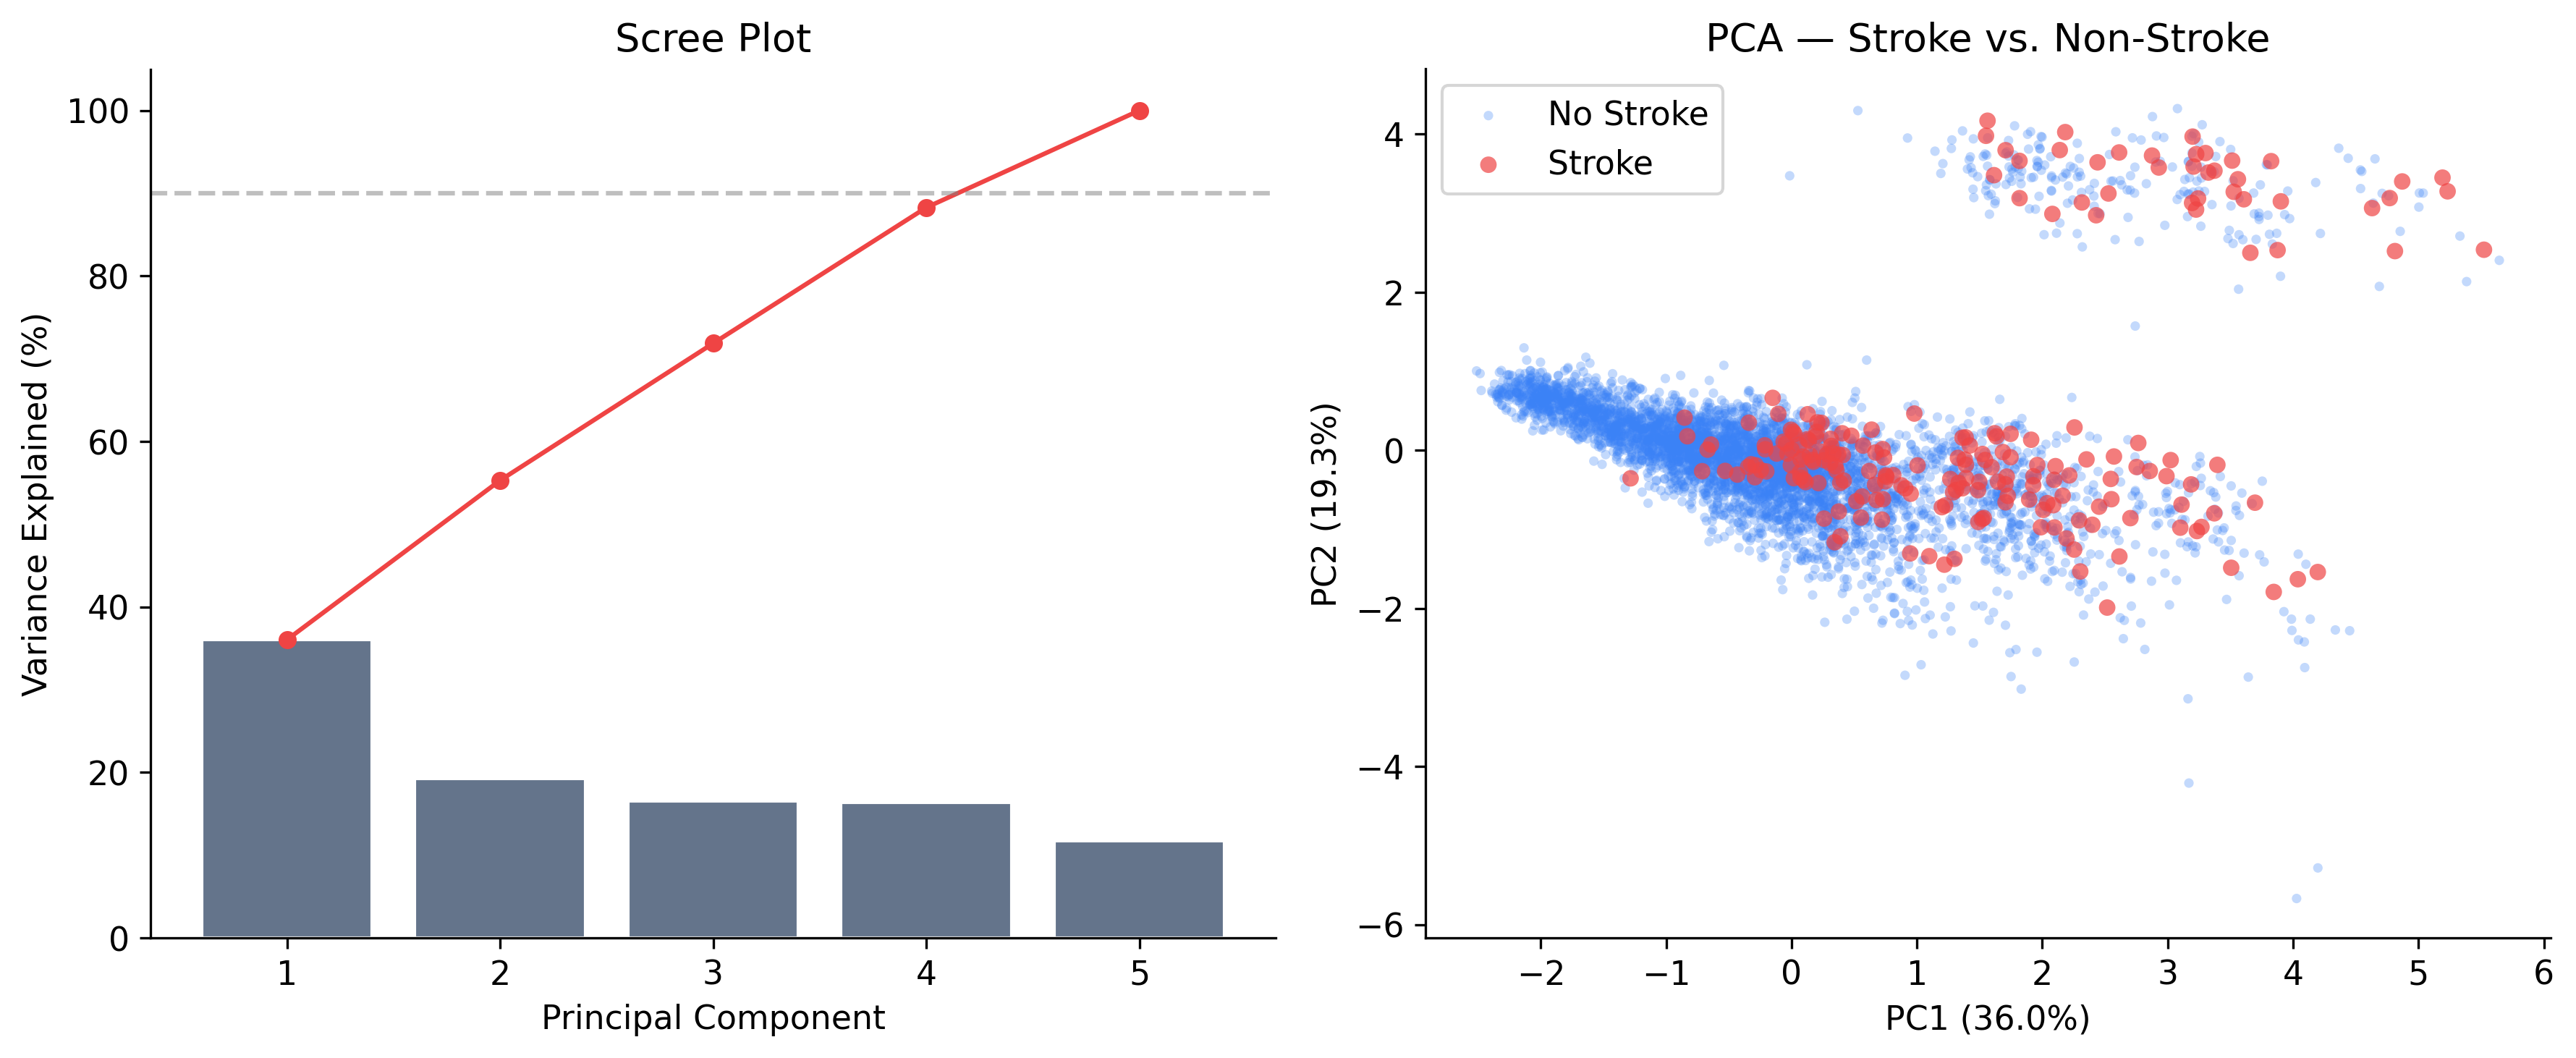
\includegraphics[width=0.7\linewidth]{06_pca.png}
  \caption{PCA projection of the dataset coloured by stroke label.}
\end{figure}

\begin{figure}[H]
  \centering
  \begin{subfigure}[b]{0.48\linewidth}
    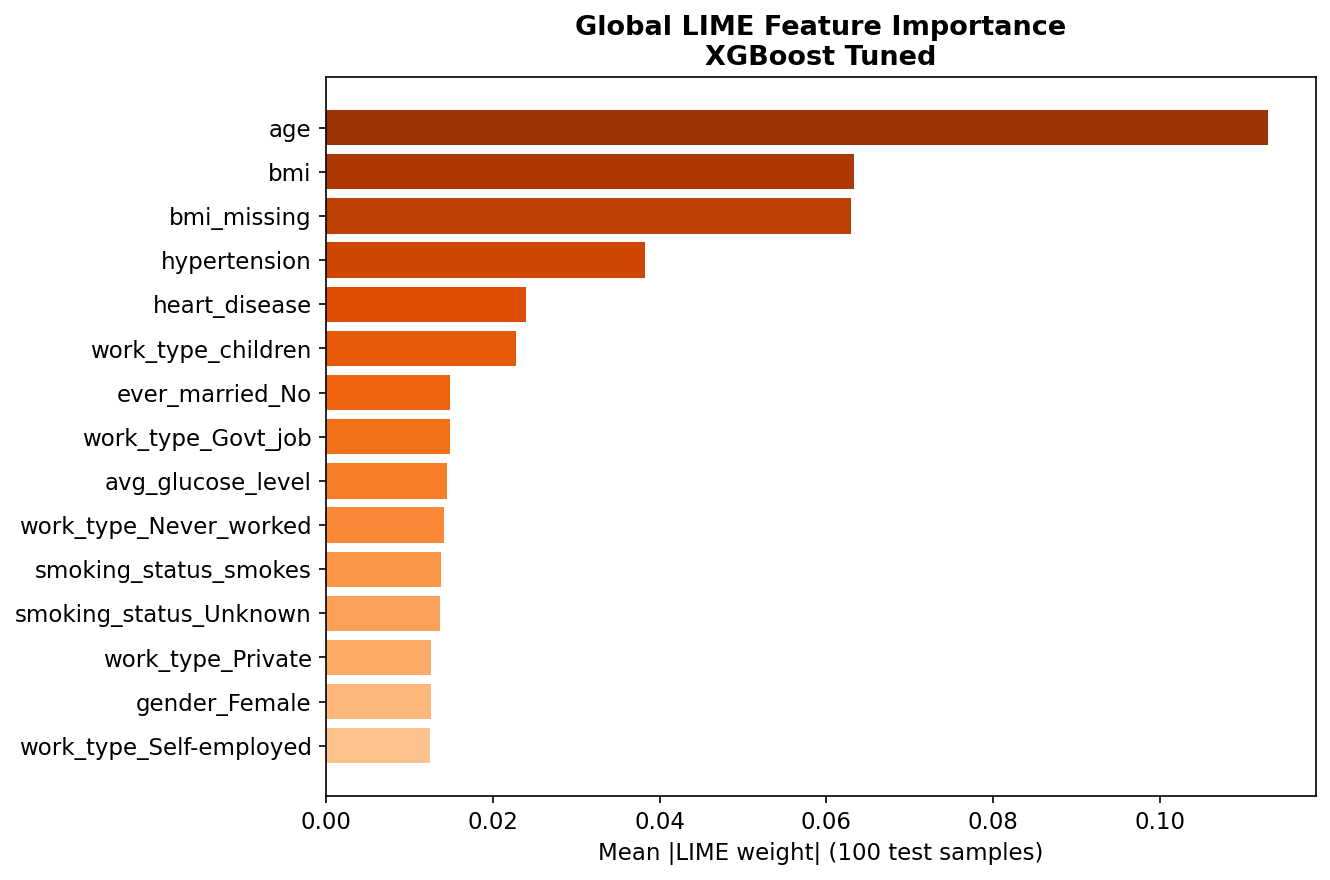
\includegraphics[width=\linewidth]{shap_lime/lime_global_bar.png}
    \caption{LIME global feature importance.}
  \end{subfigure}
  \hfill
  \begin{subfigure}[b]{0.48\linewidth}
    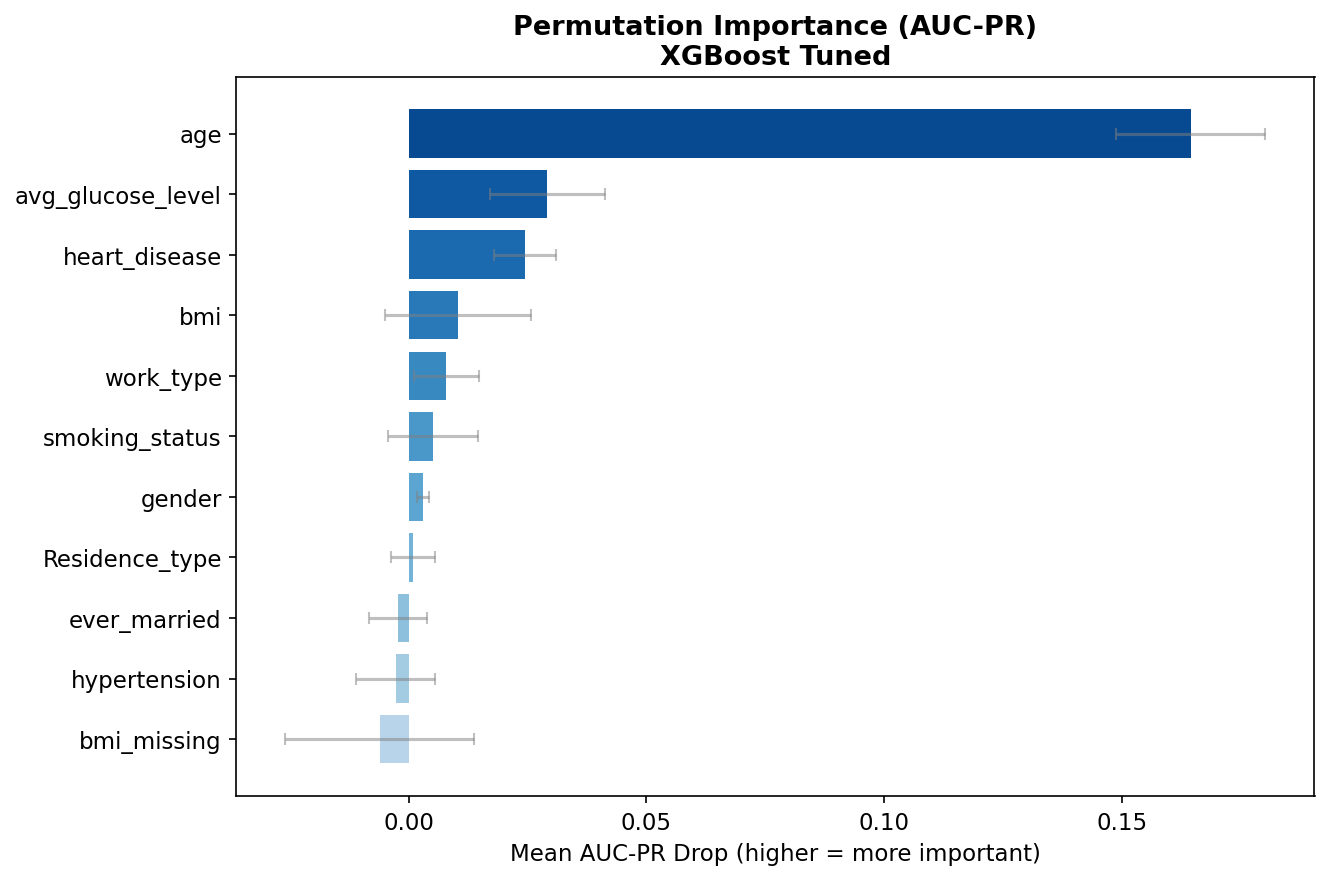
\includegraphics[width=\linewidth]{shap_lime/permutation_importance.png}
    \caption{Permutation feature importance.}
  \end{subfigure}
  \caption{Alternative feature importance estimates for the winner model.}
\end{figure}

\begin{figure}[H]
  \centering
  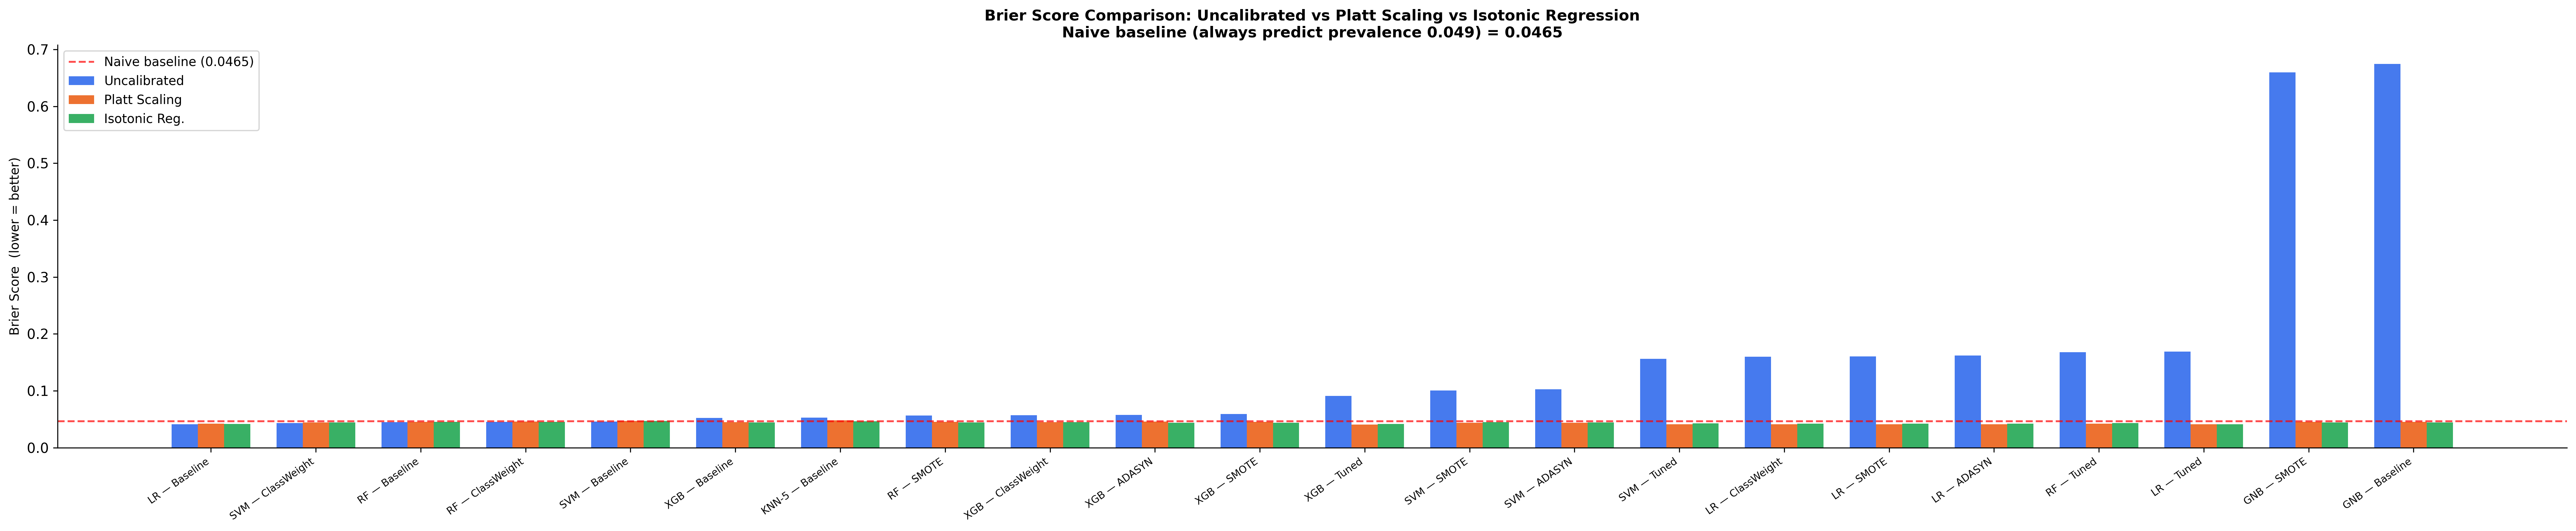
\includegraphics[width=0.72\linewidth]{brier_scores.png}
  \caption{Brier scores across all models (lower is better).}
\end{figure}

\begin{figure}[H]
  \centering
  \begin{subfigure}[b]{0.48\linewidth}
    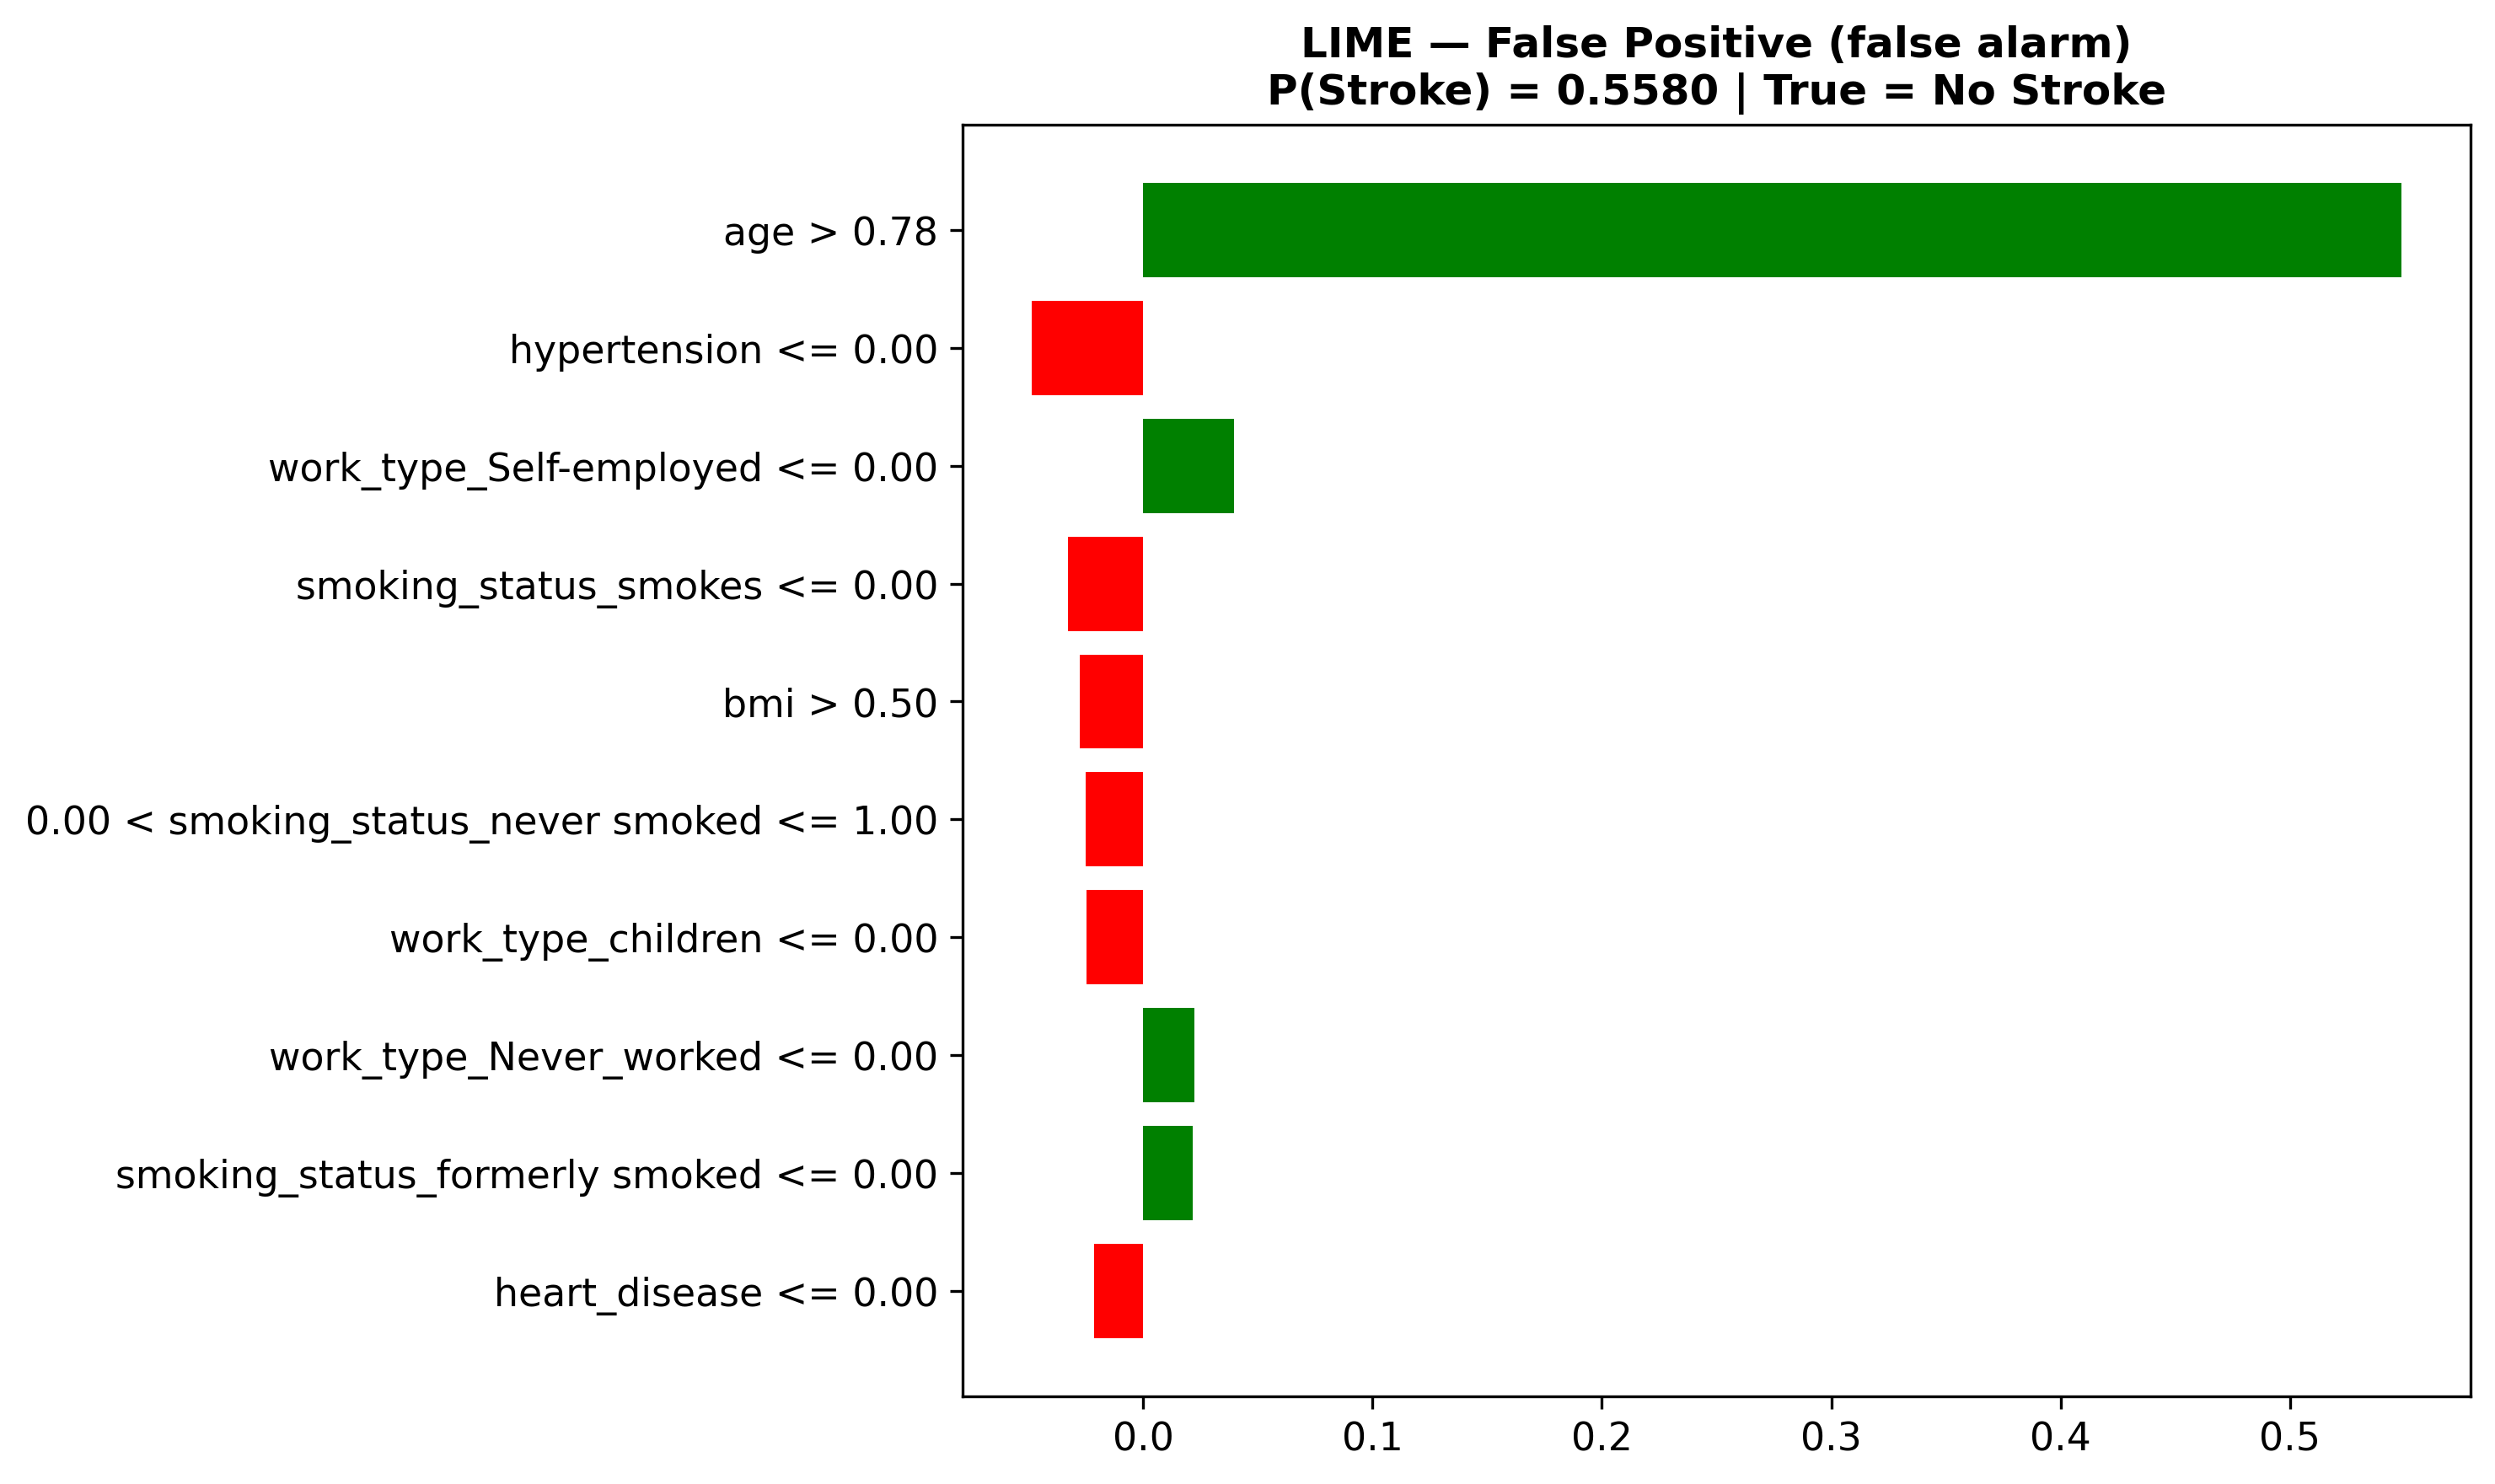
\includegraphics[width=\linewidth]{winner_analysis/lime_false_positive_false_alarm.png}
    \caption{False Positive (false alarm).}
  \end{subfigure}
  \hfill
  \begin{subfigure}[b]{0.48\linewidth}
    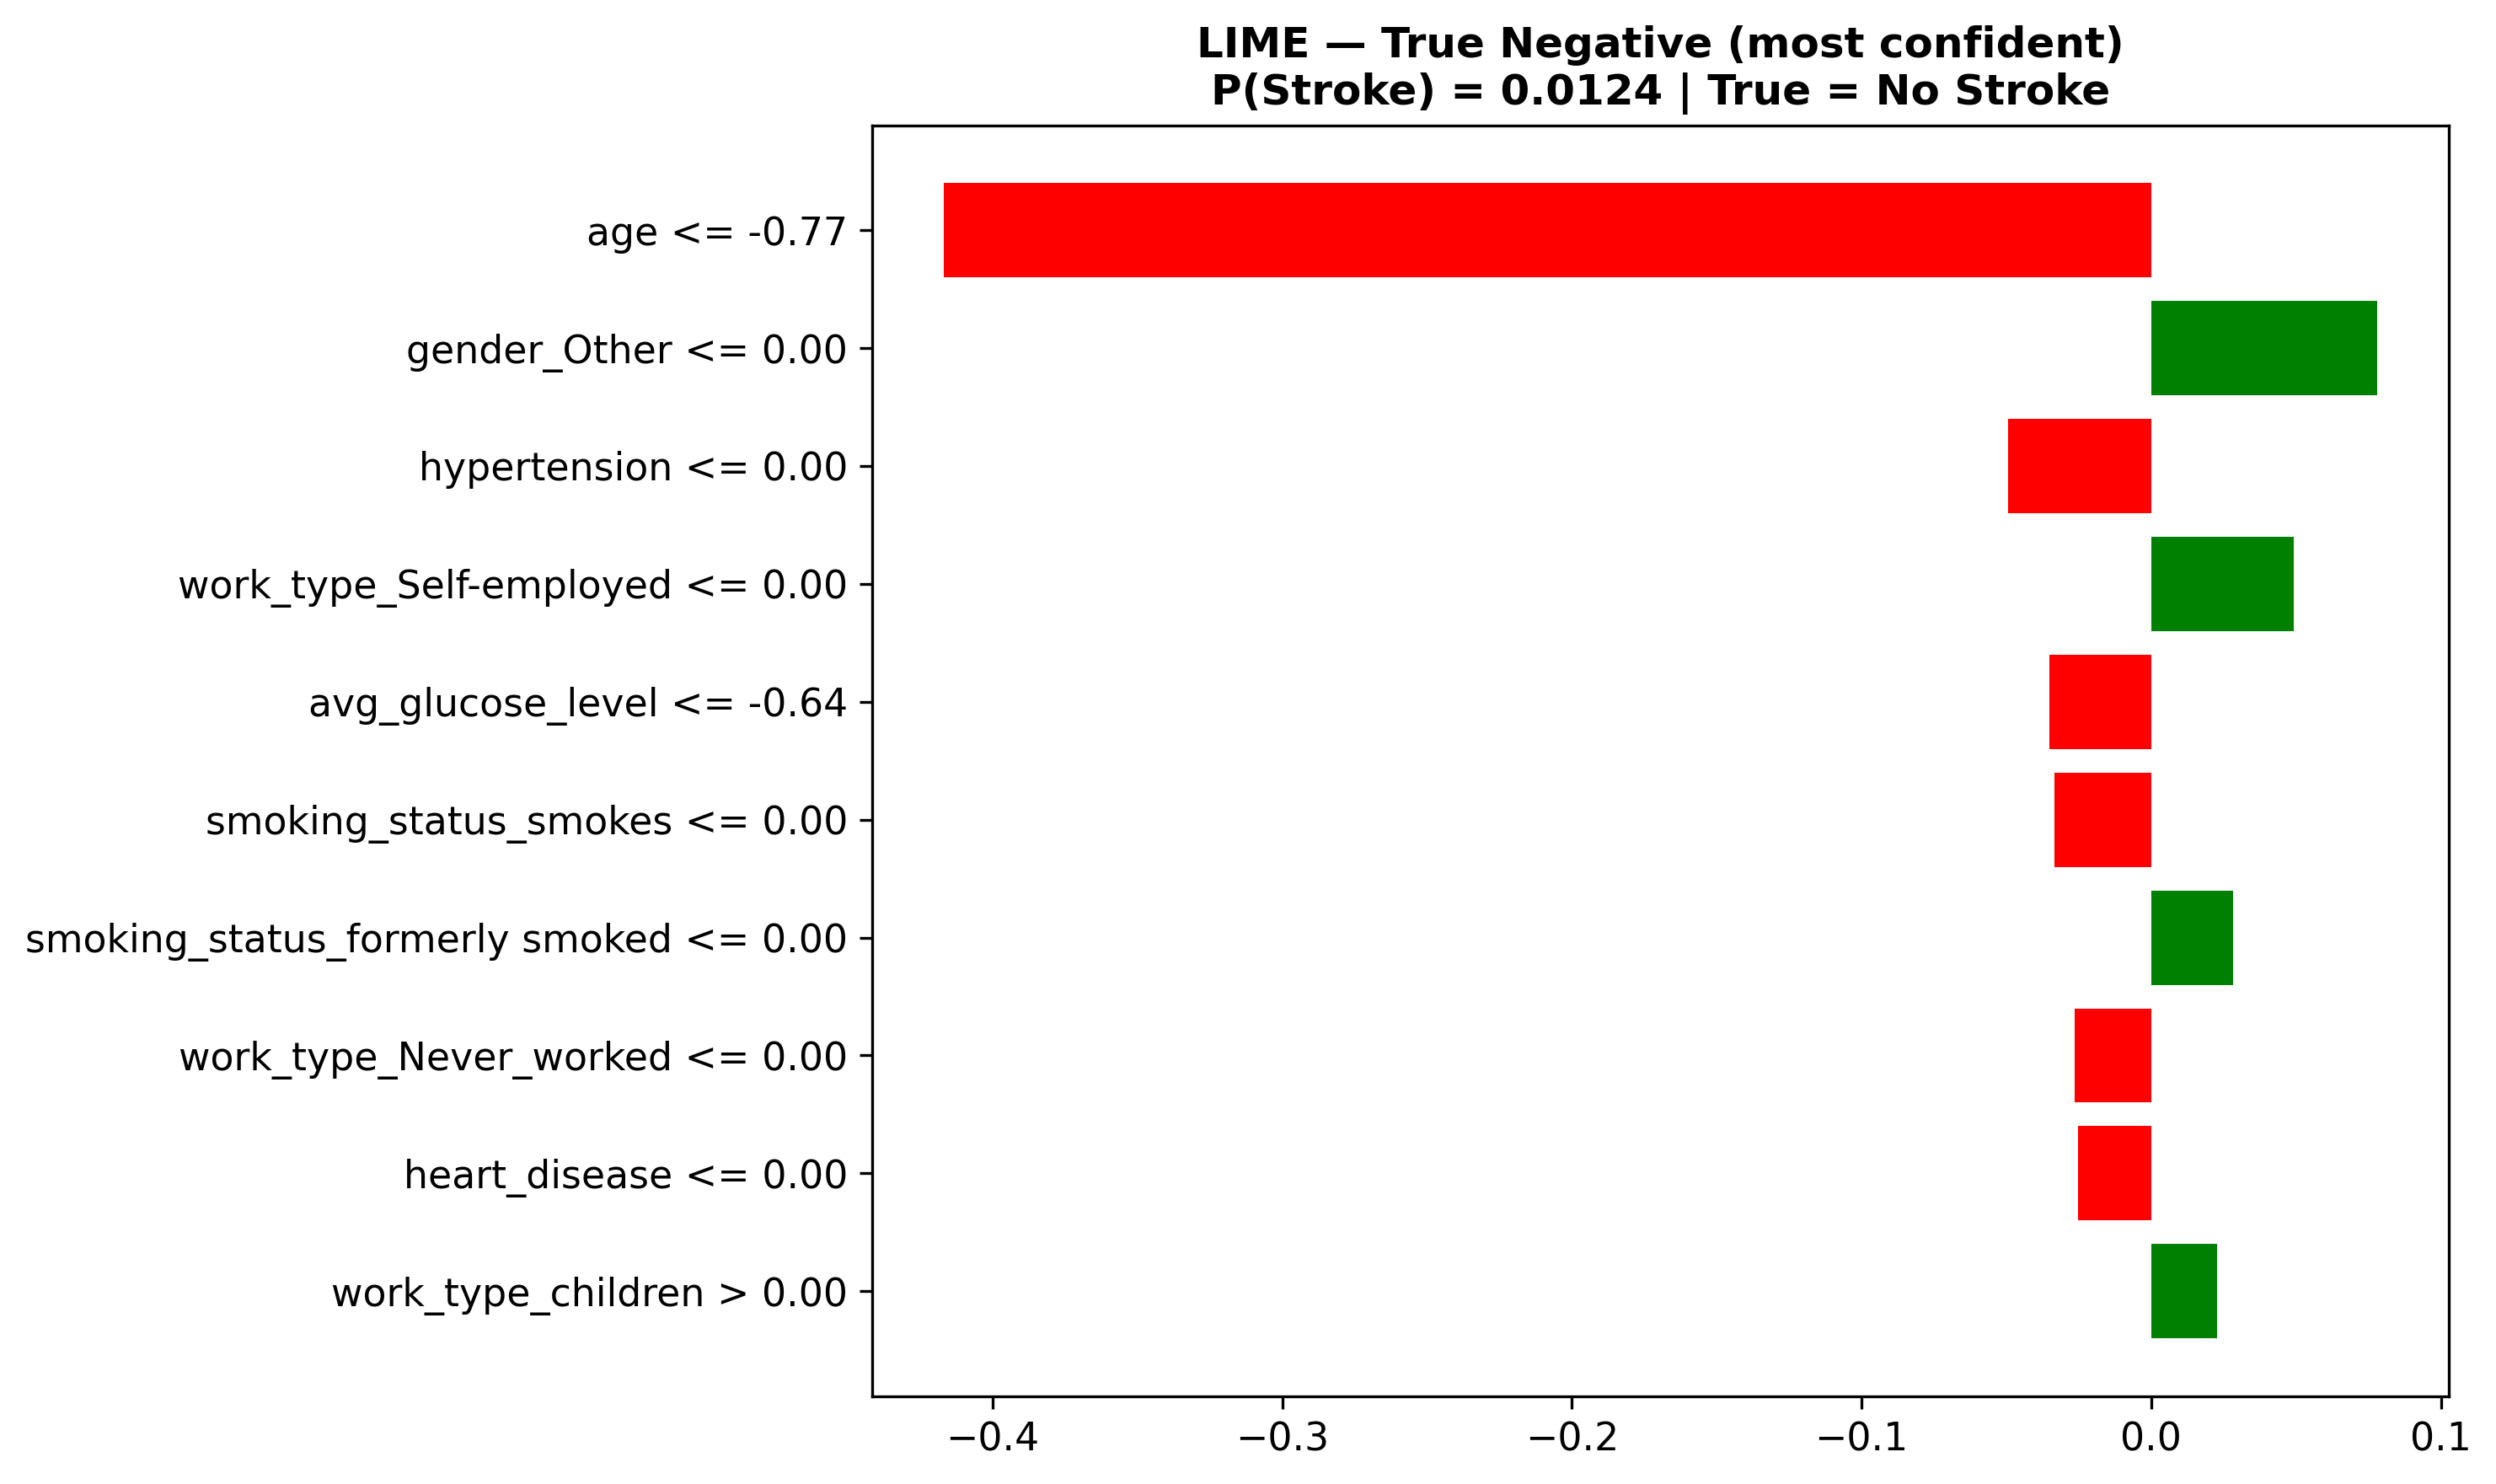
\includegraphics[width=\linewidth]{winner_analysis/lime_true_negative_most_confident.png}
    \caption{True Negative (confident healthy).}
  \end{subfigure}
  \caption{LIME local explanations for additional representative cases.}
\end{figure}

\addcontentsline{toc}{section}{References}
\begin{thebibliography}{99}

\bibitem{feigin2021global}
V.~L. Feigin \textit{et al.}
\newblock Global, regional, and national burden of stroke and its risk factors, 1990–2019: a systematic analysis for the Global Burden of Disease Study 2019.
\newblock \textit{The Lancet Neurology}, 20(10):795--820, 2021.

\bibitem{davis2006relationship}
J.~Davis and M.~Goadrich.
\newblock The relationship between precision-recall and ROC curves.
\newblock In \textit{Proceedings of ICML}, 2006.

\bibitem{fedesoriano2021stroke}
F.~Soriano.
\newblock Stroke prediction dataset (version 1).
\newblock Kaggle, 2021.
\newblock \url{https://www.kaggle.com/datasets/fedesoriano/stroke-prediction-dataset}.
\newblock Accessed: 15 March 2026.

\bibitem{chawla2002smote}
N.~V. Chawla, K.~W. Bowyer, L.~O. Hall, and W.~P. Kegelmeyer.
\newblock SMOTE: Synthetic minority over-sampling technique.
\newblock \textit{Journal of Artificial Intelligence Research}, 16:321--357, 2002.

\bibitem{he2008adasyn}
H.~He, Y.~Bai, E.~A. Garcia, and S.~Li.
\newblock ADASYN: Adaptive synthetic sampling approach for imbalanced learning.
\newblock In \textit{Proceedings of IJCNN}, pp. 1322--1328, 2008.

\bibitem{chen2016xgboost}
T.~Chen and C.~Guestrin.
\newblock XGBoost: A scalable tree boosting system.
\newblock In \textit{Proceedings of KDD}, pp. 785--794, 2016.

\bibitem{lin2017focal}
T.-Y. Lin, P.~Goyal, R.~Girshick, K.~He, and P.~Doll{\'a}r.
\newblock Focal loss for dense object detection.
\newblock In \textit{Proceedings of ICCV}, pp. 2980--2988, 2017.

\bibitem{lundberg2017shap}
S.~M. Lundberg and S.-I. Lee.
\newblock A unified approach to interpreting model predictions.
\newblock In \textit{Advances in NeurIPS}, pp. 4765--4774, 2017.

\bibitem{ribeiro2016lime}
M.~T. Ribeiro, S.~Singh, and C.~Guestrin.
\newblock ``Why should I trust you?'': Explaining the predictions of any classifier.
\newblock In \textit{Proceedings of KDD}, pp. 1135--1144, 2016.

\bibitem{sklearn}
F.~Pedregosa \textit{et al.}
\newblock Scikit-learn: Machine learning in Python.
\newblock \textit{Journal of Machine Learning Research}, 12:2825--2830, 2011.

\end{thebibliography}

\end{document}
